\documentclass[11pt,letterpaper]{article}
\usepackage[T1]{fontenc}
\usepackage[utf8]{inputenc}
\usepackage{lmodern}
\usepackage[margin=1in]{geometry}
\usepackage{graphicx}
\usepackage[table,dvipsnames]{xcolor}
\usepackage{colortbl}
\usepackage{array}
\usepackage{longtable}
\usepackage{booktabs}
\usepackage{float}
\usepackage{caption}
\usepackage{enumitem}
\usepackage{amsmath}
\usepackage{fancyhdr}
\usepackage{titlesec}
\usepackage{microtype}
\usepackage[hidelinks]{hyperref}
\definecolor{navy}{HTML}{1F3A5F}
\definecolor{teal}{HTML}{2A9D8F}
\setlist[itemize]{leftmargin=1.4em,itemsep=2pt,topsep=3pt}
\titleformat{\section}{\Large\bfseries\color{navy}}{\thesection}{0.6em}{}
\titleformat{\subsection}{\large\bfseries\color{navy}}{\thesubsection}{0.6em}{}
\titlespacing*{\section}{0pt}{16pt}{8pt}
\titlespacing*{\subsection}{0pt}{12pt}{5pt}
\captionsetup{font=small,labelfont=bf,justification=raggedright,singlelinecheck=false}
\setlength{\parindent}{0pt}
\setlength{\parskip}{5pt}
\setlength{\emergencystretch}{2em}
\sloppy
\pagestyle{fancy}
\fancyhf{}
\fancyhead[L]{\small\textcolor{gray}{Monte Carlo Counterparty Credit Risk Engine - Complete Report}}
\fancyfoot[C]{\small\thepage}
\renewcommand{\headrulewidth}{0.3pt}
\begin{document}
\begin{titlepage}
\vspace*{1.6in}
{\color{navy}\rule{\linewidth}{1.2pt}}\\[1.2em]
{\Huge\bfseries\color{navy} Monte Carlo Counterparty Credit Risk Engine\par}
\vspace{0.6em}
{\Large Methodology, calibration and results for the ESF derivatives book\par}
\vspace{0.6em}
{\color{navy}\rule{\linewidth}{1.2pt}}\\[2em]
{\large Prepared for Capitolis \textbar{} Berkeley MFE Industry Project\par}
\vspace{0.4em}
{\normalsize Valuation date 2026-08-28 \textbar{} September 2026\par}
\end{titlepage}
\section*{Abstract}
This report describes a Monte Carlo counterparty credit risk (CCR) engine for Capitolis' equity swap financing (ESF) derivatives book, which comprises 16 trades with three counterparties. The engine simulates the joint evolution of the USD short rate (a one-factor Hull-White model, with a two-factor Gaussian alternative), the JPY short rate, 37 equities and USDJPY (correlated geometric Brownian motion), reprices every trade in every scenario with the supplied pricer library, and reports Expected Exposure (EE), median PFE, Potential Future Exposure at the 99th percentile (PFE99) and Maximum PFE (MPE) by trade, by counterparty and for the portfolio on the 10-day close-out definition specified in the project brief. It prices counterparty credit risk (CVA, with DVA and FVA), computes the Basel SA-CVA capital requirement and the SA-CCR exposure at default, provides the full set of sensitivities (Greeks) of the book and of the exposure measures with the method and its cost stated, and is stress tested and backtested against realised history. The report sets out the underlying concepts from first principles, the market data and calibration, every modelling choice together with the alternatives considered, the validation performed, and the results. Every quantity is either measured from the engine on real market data as of 2026-08-28 or is an explicitly stated assumption.

\tableofcontents
\clearpage
\section*{Summary of results}
The table reports portfolio results. Exposure follows the definition in the project brief (kickoff slides 8 and 9): the movement of the netted value from its prior-day level over a 10-business-day close-out, with variation margin equal to the prior-day value and no initial margin (5,000 Latin Hypercube scenarios, PFE at the 99th percentile, one-year horizon). The uncollateralized level exposure is kept as a secondary view (3,000 scenarios).

{\footnotesize\setlength{\LTpre}{4pt}\setlength{\LTpost}{6pt}
\begin{longtable}{>{\raggedright\arraybackslash}p{\dimexpr 0.2875\linewidth-2\tabcolsep\relax}>{\raggedright\arraybackslash}p{\dimexpr 0.3125\linewidth-2\tabcolsep\relax}>{\raggedright\arraybackslash}p{\dimexpr 0.4000\linewidth-2\tabcolsep\relax}}
\toprule
\rowcolor{navy}\textbf{\textcolor{white}{Measure}} & \textbf{\textcolor{white}{Value}} & \textbf{\textcolor{white}{Meaning}} \\
\endhead
Peak EE (close-out exposure) & \$11.6M at 2026-09-20 & Highest average 10-day close-out exposure within one year \\
\rowcolor{gray!9}Peak median PFE (close-out) & \$8.2M & Typical (50th percentile) close-out exposure at its highest date \\
Maximum PFE99, MPE (close-out) & \$51.0M at 2026-09-20 & Highest 99th-percentile close-out exposure within one year \\
\rowcolor{gray!9}Portfolio MPE against the sum of counterparty MPEs & \$51.0M against \$65.1M & No netting across counterparties, and peaks that coincide: little diversification (Section 7.2) \\
Current exposure today (uncollateralized) & \$129.8M & Loss if every counterparty defaulted today with no margin, after netting \\
\rowcolor{gray!9}MPE99, uncollateralized (secondary view) & \$201.9M at 2026-10-09 & Highest 99th-percentile level exposure over the life of the book \\
Concentration & 96\% of current exposure is CPTY\_C & A single \$500M bond forward (BF\_0003) dominates \\
\rowcolor{gray!9}Time profile & Most exposure has run off by December 2026 & Trades mature; a small Bond TRS tail runs to January 2028 \\
CVA, close-out exposure (BBB proxy) & \$11,747 & Price of counterparty default risk on the margined close-out exposure, unilateral (Section 8) \\
\rowcolor{gray!9}CVA, uncollateralized exposure & \$247,133 & The same on the level exposure: the price if no margin were ever called \\
DVA and FVA (close-out) & \$11,244 and \$503 & On assumed own credit and funding spreads (Section 8.5) \\
\rowcolor{gray!9}SA-CVA capital & \$0.10M close-out; \$2.23M uncollateralized (RWA \$1.2M; \$27.8M) & Basel standardised approach on the two exposure definitions; dominated by counterparty credit spread risk (Section 8.4) \\
SA-CCR exposure at default & \$260.3M & Regulatory EAD, uncollateralized; dominated by the replacement cost of BF\_0003 (Section 8.6) \\
\rowcolor{gray!9}Greeks & t = 0 book Greeks; sensitivities of EE, median PFE and PFE99 to equities, USDJPY, USD rates and volatilities & Complete, by netting set, method and cost stated (Section 9) \\
Stress test & 11 scenarios; largest close-out MPE \$60.7M (Rates -200bp) & Hypothetical and historical replays, by product and along the time path (Section 7.10) \\
\rowcolor{gray!9}Backtest (Kupiec) & 99\% equity leg: 4/6/2 exceptions against 2.4/2.4/2.4 expected in the three netting sets & Realised 10-day moves against the model's quantiles, out of sample (Section 11.7) \\
\bottomrule
\end{longtable}}

\textbf{Principal modelling choices} (each is justified in Section 10):

\begin{itemize}
\item Monte Carlo under the risk-neutral measure. USD short rate: one-factor Hull-White fitted exactly to today's SOFR curve, with the Bloomberg long end spliced beyond the last futures contract and sigma fitted to the realised volatility of 2y-30y Treasury yields. Equities and USDJPY: correlated geometric Brownian motion driven by the simulated rates; a two-factor Gaussian (G2++) alternative is implemented and compared.
\item Exposure: the brief's definition, max(V(t + 10bd) - V(t - 1bd), 0) with variation margin equal to the prior-day value, per trade and per counterparty over one year; the uncollateralized level exposure is kept as a secondary view.
\item Correlation: one static 40x40 matrix (37 equities, USDJPY, USD rate on 10-year-yield shocks, JPY rate) estimated from 616 aligned daily returns and applied through a Cholesky factor; a PCA factor model (5 factors) is provided as an alternative and its cost and benefit are measured (Section 4.4).
\item Sampling and size: Latin Hypercube sampling (lowest error of the five methods tested) with N = 5,000 scenarios for standard reporting, N = 1,000 for iteration and N = 10,000 for limit sign-off (Section 5.5).
\item Dates: standard market pillar dates (O/N to 10Y) with every trade's own reset and maturity date, and the t - 1bd and t + 10bd nodes required by the exposure definition, on the grid.
\item Mean reversion: a = 0.0167 for USD from the swaption cube; for JPY the lower bound a = 0.001, because real JPY volatility rises with tenor (three independent sources).
\item JPY: a negative-rate-capable Hull-White factor (sigma from the real JPY OIS history, correlated with the USD rate, USDJPY and the equities) drives the drift of JPY-listed names and USDJPY.
\item Credit: unilateral CVA (MAR50.32) with counterparty spreads proxied from ICE BofA bond indices by an assumed BBB rating and 60\% LGD, computed on both exposure definitions; DVA and FVA on assumed own credit and funding spreads; SA-CVA capital and SA-CCR EAD.
\item Model risk: attribution of every correction, a one-at-a-time perturbation study, a structured stress test and a Kupiec backtest (Sections 7.3, 7.9, 7.10, 11.7).
\end{itemize}
\clearpage
\section{The problem from scratch}
\subsection{What is counterparty credit risk?}
A derivative is a contract whose value changes as markets move. If we hold a contract with positive value to us, the counterparty owes us that value. If the counterparty then defaults, we lose (some of) it. \textbf{Counterparty credit risk (CCR)} is that loss risk. It is not the same as market risk: market risk is about our profit and loss moving; CCR is about whether the other side can pay when the contract is in our favour.

Two properties make CCR different from ordinary risk measures:

\begin{itemize}
\item \textbf{It is one-sided.} If a contract is worth -5M to us we owe them; their default does not cost us that 5M back. So exposure is max(V, 0), a call option on the value (Figure 1).
\item \textbf{It is about the future.} A default can happen at any date, so what matters is not today's value but the distribution of what the book could be worth on every future date. That needs simulation.
\end{itemize}
\begin{figure}[H]
\centering
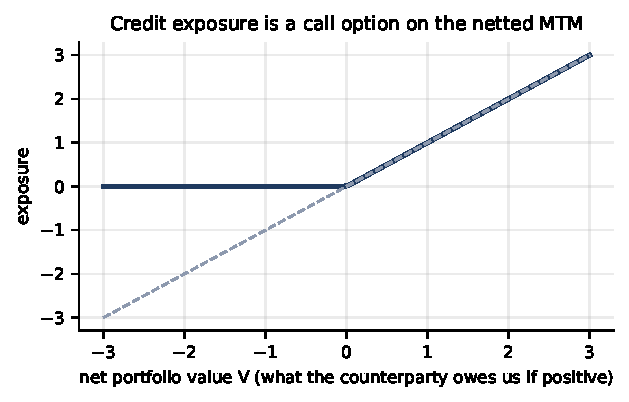
\includegraphics[width=\linewidth]{figures/fig01.pdf}
\caption{Exposure is the positive part of the net value V. Negative value is not a credit exposure.}
\end{figure}
\subsection{Netting}
Trades with the same counterparty under one legal netting agreement are combined before applying max(V,0): a +10M trade and a -6M trade give exposure 4M, not 10M. Netting never crosses counterparties. The portfolio exposure is therefore the \emph{sum over counterparties} of each counterparty's own max(sum of trade values, 0).

\subsection{The four measures reported}
{\footnotesize\setlength{\LTpre}{4pt}\setlength{\LTpost}{6pt}
\begin{longtable}{>{\raggedright\arraybackslash}p{\dimexpr 0.1948\linewidth-2\tabcolsep\relax}>{\raggedright\arraybackslash}p{\dimexpr 0.3377\linewidth-2\tabcolsep\relax}>{\raggedright\arraybackslash}p{\dimexpr 0.4675\linewidth-2\tabcolsep\relax}}
\toprule
\rowcolor{navy}\textbf{\textcolor{white}{Measure}} & \textbf{\textcolor{white}{Definition}} & \textbf{\textcolor{white}{How to read it}} \\
\endhead
Exposure profile V+(t) & max(net MTM, 0) at each future date t, in each simulated scenario & The raw object; everything below summarises its distribution across scenarios \\
\rowcolor{gray!9}Close-out exposure (headline) & max( V(t + 10bd) - V(t - 1bd), 0 ), netted by counterparty & The brief's definition (slides 8 and 9): variation margin is the prior-day NPV, no initial margin, 10-business-day close-out. EE, median PFE, PFE99 and MPE are computed on it unless labelled uncollateralized \\
EE (Expected Exposure) & Mean of exposure across scenarios at date t & Average loss if default happens at t; used for pricing credit charges (CVA) \\
\rowcolor{gray!9}Median PFE & 50th percentile of exposure across scenarios at date t & The typical scenario. Exposure is floored at zero: the median is below EE when exposure is right-skewed (most scenarios small, a few large) and can be exactly zero when most scenarios are out of the money; it can sit slightly above EE when the book is almost always in the money, as for the dominant CPTY\_C forward \\
PFE99 (Potential Future Exposure) & The 99th percentile of exposure at date t & In 99 of 100 scenarios exposure at t is below this level. Used to set limits \\
\rowcolor{gray!9}MPE (Maximum PFE) & Peak of the PFE curve over all dates & One number to set a counterparty limit against \\
\bottomrule
\end{longtable}}

\textbf{Confidence level.} PFE is reported at the 99th percentile throughout, together with the median PFE (the 50th percentile of the same exposure distribution), which describes the typical scenario.

\begin{figure}[H]
\centering
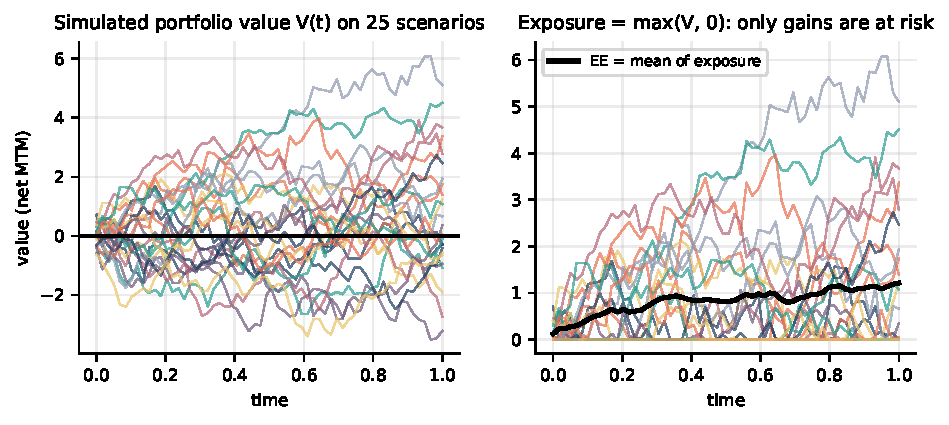
\includegraphics[width=\linewidth]{figures/fig02.pdf}
\caption{Left: simulated values of a portfolio through time. Right: the same paths after applying max(V,0); EE is their average.}
\end{figure}
\begin{figure}[H]
\centering
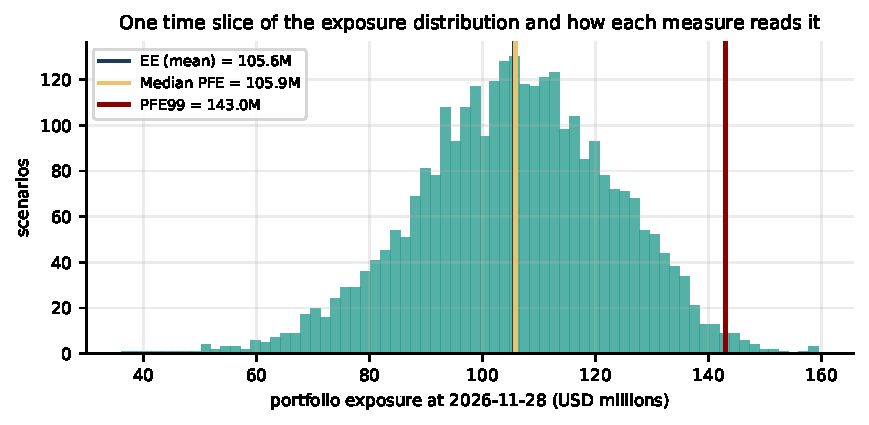
\includegraphics[width=\linewidth]{figures/fig03.pdf}
\caption{The real portfolio exposure distribution $\sim$3 months out, with EE, median PFE and PFE99 marked. The long right tail is why EE, median PFE and PFE99 differ so much.}
\end{figure}
\subsection{Why Monte Carlo}
The value of the book at a future date depends on the future levels of $\sim$40 market variables (37 stock prices, USDJPY, interest rates) that move together. There is no closed formula for the distribution of a netted, path-dependent-schedule book. Monte Carlo solves this by: (1) simulating thousands of joint futures for all the variables; (2) fully re-pricing every trade in every simulated future at every date; (3) netting; (4) reading off the distribution. The cost is that the answer has sampling noise, which we measure and control (Sections 5.4 and 5.5).

\subsection{Real-world versus risk-neutral simulation}
Simulating under the \emph{risk-neutral} measure (drift = short rate minus dividends) is the pricing-consistent choice used for CVA and for exposure numbers that must be consistent with today's market prices. The alternative, real-world (physical) drift, is used for regulatory PFE limits and would add a risk premium to the drifts. We use risk-neutral because it needs no extra unobservable inputs and is verified by a martingale test (Section 11). Because the horizon is short (under two years) and most positions are financed at the same rates, the difference between the two drifts is small relative to volatility.

\clearpage
\section{The trade book}
The book has \textbf{16 trades} with \textbf{3 counterparties} (CPTY\_A, CPTY\_B, CPTY\_C), referencing 37 unique equities (31 USD-quoted, 6 JPY-quoted) and 5 US Treasury bonds. Trade files are supplied by Capitolis in trade\_data/.

\subsection{The three instruments}
\textbf{Equity Total Return Swap (TRS).} One party pays the total return of a basket of shares (price change plus dividends) and receives a funding leg (SOFR plus a spread, or a fixed rate) on a financed amount. Value = equity leg minus funding leg:

{\fontsize{7.2}{8.8}\selectfont
\begin{verbatim}
equity leg  = sum_i shares_i * DF(end) * (F_i(end) - basis_i)     F(t) = S(t)/DF(end)
funding leg = sum_k rate_k * Notional * tau_k * DF(t_k)            rate_k = SOFR_fwd + spread  (or fixed)
NPV         = equity leg - funding leg
\end{verbatim}}
Eight of these (EQTRS\_0001-0008), all `pay\_equity' from our side, so we are long the funding leg and short the equity return: our value rises when the shares fall. Two are JPY \emph{compo} trades: both legs settle in USD but the equity leg pays the return of the USD value of a JPY share (S\_JPY x USDJPY), so equity and FX risk both matter.

\textbf{Bond Forward.} An agreement to sell/buy a Treasury at a fixed clean price on a future date: NPV = sign x (notional/par) x DF(T) x (forward clean price - strike). The forward price is the spot financed at the repo rate less coupons in the window. Four of these, all short. BF\_0003 has a 500M notional and dominates CPTY\_C.

\textbf{Bond TRS.} Same idea as an equity TRS but on a bond: return leg (price change plus coupons) versus a funding leg over a reset schedule. Four of these.

{\footnotesize\setlength{\LTpre}{4pt}\setlength{\LTpost}{6pt}
\begin{longtable}{>{\raggedright\arraybackslash}p{\dimexpr 0.2097\linewidth-2\tabcolsep\relax}>{\raggedright\arraybackslash}p{\dimexpr 0.1935\linewidth-2\tabcolsep\relax}>{\raggedright\arraybackslash}p{\dimexpr 0.1774\linewidth-2\tabcolsep\relax}>{\raggedright\arraybackslash}p{\dimexpr 0.1774\linewidth-2\tabcolsep\relax}>{\raggedright\arraybackslash}p{\dimexpr 0.2419\linewidth-2\tabcolsep\relax}}
\toprule
\rowcolor{navy}\textbf{\textcolor{white}{Trade}} & \textbf{\textcolor{white}{Type}} & \textbf{\textcolor{white}{Counterparty}} & \textbf{\textcolor{white}{Ends}} & \textbf{\textcolor{white}{Today's NPV}} \\
\endhead
EQTRS\_0001 & EquityTRS & CPTY\_A & 2026-10-14 & -5,547,056 \\
\rowcolor{gray!9}EQTRS\_0002 & EquityTRS & CPTY\_A & 2026-10-09 & -1,076,056 \\
EQTRS\_0003 & EquityTRS & CPTY\_A & 2026-10-16 & 9,921,581 \\
\rowcolor{gray!9}EQTRS\_0004 & EquityTRS & CPTY\_B & 2026-11-02 & -873,451 \\
EQTRS\_0005 & EquityTRS & CPTY\_B & 2026-10-09 & 148,605 \\
\rowcolor{gray!9}EQTRS\_0006 & EquityTRS & CPTY\_B & 2026-10-30 & 1,629,065 \\
EQTRS\_0007 & EquityTRS & CPTY\_C & 2026-10-23 & -373,630 \\
\rowcolor{gray!9}EQTRS\_0008 & EquityTRS & CPTY\_C & 2027-07-22 & 2,217,998 \\
BF\_0001 & BondForwardTrade & CPTY\_A & 2026-10-30 & 512,531 \\
\rowcolor{gray!9}BF\_0002 & BondForwardTrade & CPTY\_A & 2026-11-08 & -357,505 \\
BF\_0003 & BondForwardTrade & CPTY\_C & 2026-12-06 & 121,262,854 \\
\rowcolor{gray!9}BF\_0004 & BondForwardTrade & CPTY\_C & 2026-10-25 & 1,973,388 \\
BTRS\_0001 & BondTRS & CPTY\_A & 2028-01-15 & 119,460 \\
\rowcolor{gray!9}BTRS\_0002 & BondTRS & CPTY\_B & 2027-01-15 & 210,278 \\
BTRS\_0003 & BondTRS & CPTY\_B & 2027-04-09 & 28,844 \\
\rowcolor{gray!9}BTRS\_0004 & BondTRS & CPTY\_C & 2026-11-04 & 36,376 \\
\bottomrule
\end{longtable}}

\begin{figure}[H]
\centering
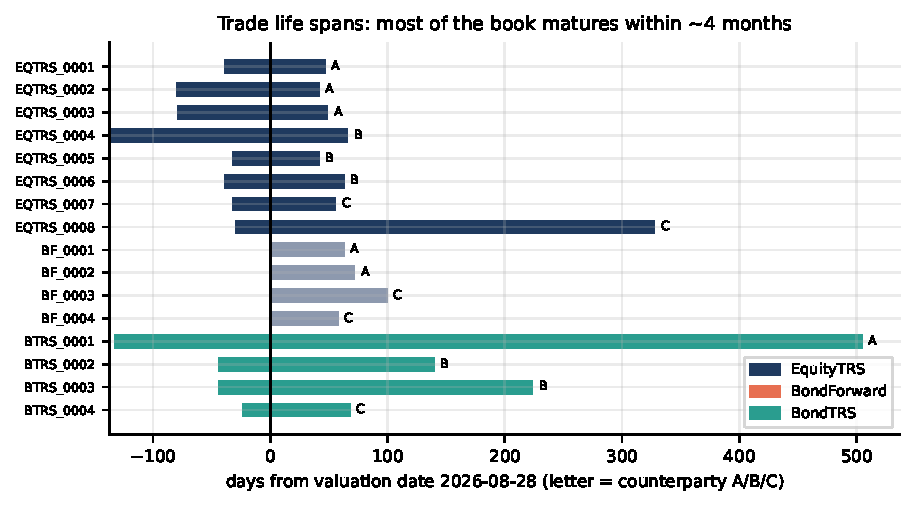
\includegraphics[width=\linewidth]{figures/fig04.pdf}
\caption{Life span of every trade. Nearly all exposure will therefore disappear within four months; only BTRS\_0001 and EQTRS\_0008 run past mid-2027.}
\end{figure}
\begin{figure}[H]
\centering
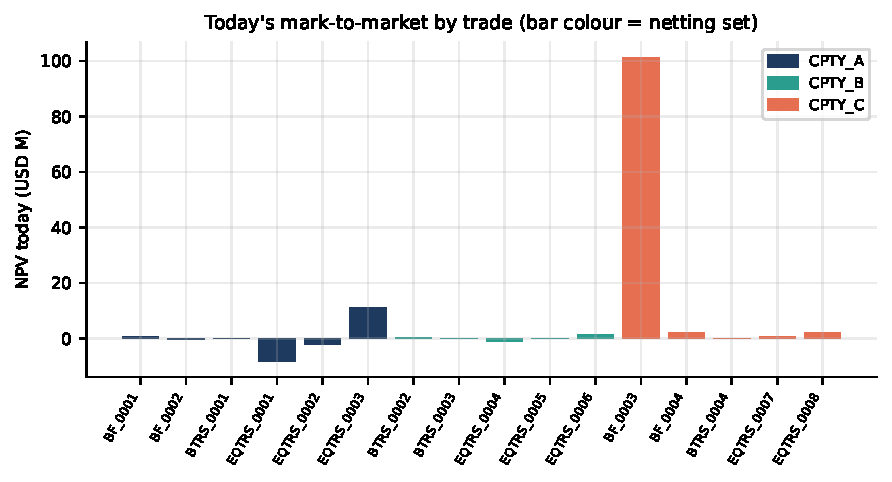
\includegraphics[width=\linewidth]{figures/fig05.pdf}
\caption{Today's mark-to-market per trade. CPTY\_C's total is dominated by BF\_0003 (+121M); CPTY\_B nets to a small positive, so its exposure today is small.}
\end{figure}
\subsection{Pricing library (the `contract')}
The trades are priced by capitolis\_pricers, a self-contained standard-library re-implementation of QuantLib/ORE-style discounted cash flows supplied with the project. Every pricer is a pure function \texttt{npv = pricer.npv(MarketState)}. Our simulation therefore never contains pricing logic of its own: at every (scenario, date) we build a \texttt{MarketState} from simulated inputs (a discount curve, equity spots, an FX curve) and call the same \texttt{.npv()}. This is a deliberate design choice: the pricers were independently reviewed (docs/notes/pricer\_review.md), so any error in the exposure numbers cannot hide inside re-implemented pricing.

\clearpage
\section{Market data: what we used and why}
Every risk factor needs both a \emph{starting value} and \emph{dynamics} (volatility, correlation, mean reversion). We prefer real, verifiable data; where none exists we use a labelled assumption.

{\scriptsize\setlength{\LTpre}{4pt}\setlength{\LTpost}{6pt}
\begin{longtable}{>{\raggedright\arraybackslash}p{\dimexpr 0.1948\linewidth-2\tabcolsep\relax}>{\raggedright\arraybackslash}p{\dimexpr 0.2857\linewidth-2\tabcolsep\relax}>{\raggedright\arraybackslash}p{\dimexpr 0.2338\linewidth-2\tabcolsep\relax}>{\raggedright\arraybackslash}p{\dimexpr 0.2857\linewidth-2\tabcolsep\relax}}
\toprule
\rowcolor{navy}\textbf{\textcolor{white}{Input}} & \textbf{\textcolor{white}{Source}} & \textbf{\textcolor{white}{Used for}} & \textbf{\textcolor{white}{Note}} \\
\endhead
USD discount curve & Databento: CME SR3/SR1 SOFR futures (33 live contracts), bootstrapped by us & Discounting, forwards, Hull-White fit & Validated against Treasury.gov par curve (spread 13bp at 1M to 46bp at 10Y) \\
\rowcolor{gray!9}37 equity spots and dividend yields & yfinance & GBM start values and drift & Keyed by ISIN; BRK.B ticker mismatch found and fixed \\
USDJPY spot & yfinance & FX start value &  \\
\rowcolor{gray!9}Volatilities (39) & Realised, 3 years of daily data; USD rate sigma fitted to Treasury yield vols & Diffusion size & No options data available; documented proxy \\
Correlation matrix 39x39 & 616 dates where all series exist (inner join) & Cholesky / PCA & Verified positive semi-definite \\
\rowcolor{gray!9}SOFR level history & FRED & USD-JPY correlation; rate-vol comparison & From April 2018 \\
Treasury constant-maturity yields, 3M to 30Y, 1981 to date & FRED (DGS series) & USD rate sigma and correlations; G2++ calibration; backtest; stress replays & Public \\
\rowcolor{gray!9}Long price and USDJPY history, 2014-2026 & yfinance & Backtest and historical stress windows & Public \\
USD SOFR zero curve (long end beyond the last futures contract) & Bloomberg one-time export, 2026-08-31 & Spliced onto the futures curve beyond about 6.5 years & Licensed data: derived numbers only \\
\rowcolor{gray!9}JPY OIS par-rate history, 35 tenors, 2011-2026 & Bloomberg export provided by the project team (data/raw/sources/JPY.xlsx) & JPY curve, JPY factor volatility, JPY-USD differential, mean-reversion test & Licensed data: only derived quantities are reported \\
USD and JPY swaption cubes, USDJPY forwards & Bloomberg one-time export, 2026-08-31 snapshot & USD mean reversion, cross-checks, FX forwards & Licensed data: only derived quantities are reported \\
\rowcolor{gray!9}TONA (JPY overnight rate) & Bank of Japan public API, daily from 1998 & JPY rate vol, USD-JPY correlation & Includes real negative-rate years \\
JGB par yields 1Y-40Y & Japan Ministry of Finance, daily from 1974 & JPY mean-reversion test & Public \\
\bottomrule
\end{longtable}}

\subsection{The USD curve}
Databento provides the futures, not a ready OIS curve, so we build one: each 3-month SOFR future price gives an implied forward rate (100 - price) for its reference quarter; chaining consecutive quarters multiplies discount factors. The futures end about 6.5 years out. Beyond the last contract the curve now follows the forward structure of the Bloomberg USD SOFR zero curve (below); earlier versions extrapolated flat, which was one of the defects corrected in this version (Section 12). Two real bugs in the futures bootstrap were found by cross-checking with the Treasury curve (Section 12). The curve is the starting point of the Hull-White model and the discount curve at t=0.

\begin{figure}[H]
\centering
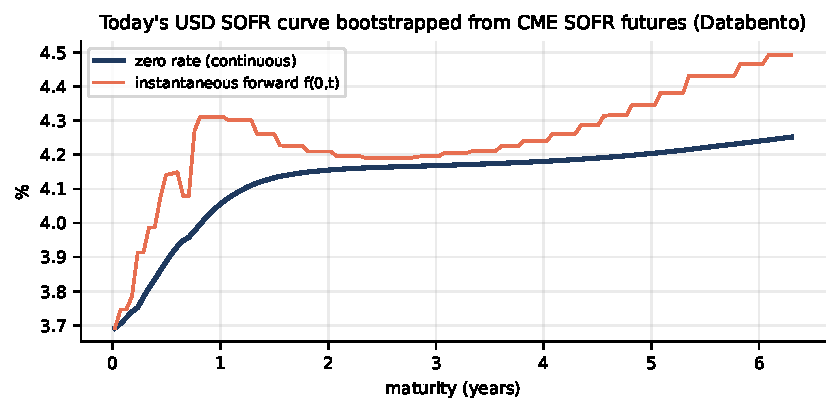
\includegraphics[width=\linewidth]{figures/fig06.pdf}
\caption{The bootstrapped USD SOFR curve, with the long end spliced beyond the last futures contract. The upward slope (zero rate about 3.7\% at the front, above 4\% by 6 years) means forwards exceed spot rates.}
\end{figure}
The SOFR-futures curve ends at about 6.6 years and was previously extrapolated flat in the zero rate. That understates the discounting of the long-dated Treasury underlying BF\_0003 (maturity 2049): at 20 years the flat extrapolation gives a zero rate of 4.27\%, against 4.65\% on the spliced curve. Beyond the last futures pillar the curve now follows the forward structure of the Bloomberg USD SOFR zero curve (2026-08-31 snapshot, re-based to our 2026-08-28 reference date), joined continuously at the last futures pillar; inside the futures range nothing changes.

\begin{figure}[H]
\centering
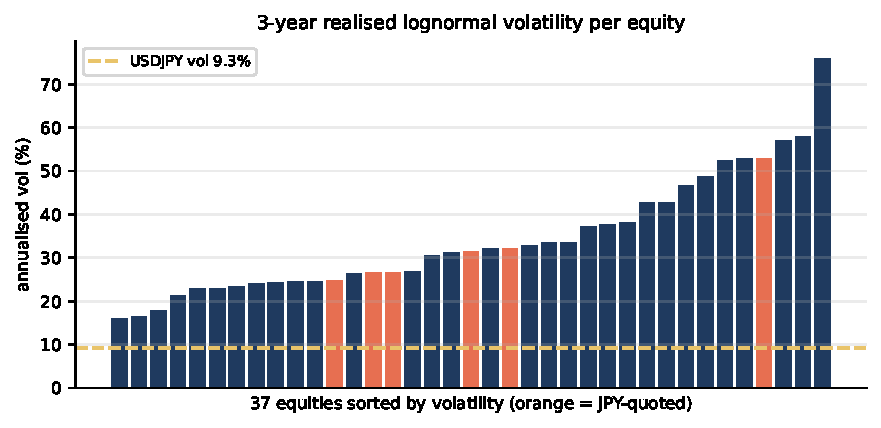
\includegraphics[width=\linewidth]{figures/fig07.pdf}
\caption{Zero-rate curve before and after splicing the long end. Inside the futures range the two coincide exactly.}
\end{figure}
The effect on the mark of BF\_0003 is large because a 500M notional on a 22-year bond has a duration of about 13: its NPV moves from \$101.4M on the flat extrapolation to \$121.3M on the spliced curve, within half a percent of the \$120.9M obtained by repricing on Bloomberg's own zero curve.

\subsection{Volatilities}
Volatility is the annualised standard deviation of daily changes over the last three years (log returns for equities and FX; simple differences for rates, because rate LEVELS near or below zero make log returns meaningless). The USD rate volatility is treated separately, below.

\begin{figure}[H]
\centering
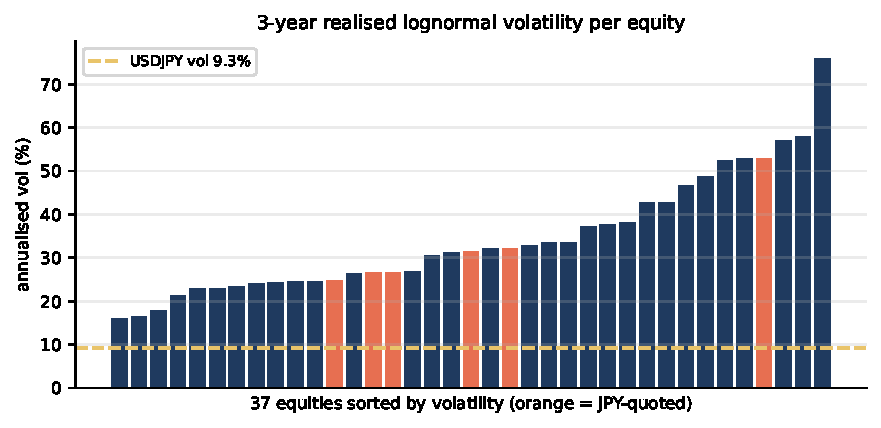
\includegraphics[width=\linewidth]{figures/fig08.pdf}
\caption{Realised volatility spans an order of magnitude across the 37 names. A few names carry 50-76\% vol, which dominates tail exposure of the trades that reference them.}
\end{figure}
The USD Hull-White volatility was set equal to the realised volatility of the overnight SOFR fixing (63bp). That number is small because the overnight rate moves in steps on Fed dates, and it says little about how far the 2- to 30-year yields, on which the book depends, move. Over the same three-year window the annual normal vol of Treasury yields was 91/93/86/83/81 bp for the 2y to 30y tenors. In a one-factor Hull-White model the zero rate at tenor T has normal vol sigma (1 - exp(-aT))/(aT), so sigma is now fitted by least squares to the realised 2y-30y yield vols with the mean reversion held at its swaption-calibrated value: sigma = 96bp. The rate factor's correlations with equities and USDJPY are re-estimated on 10-year yield changes for the same reason (SOFR fixings correlate with nothing).

\begin{figure}[H]
\centering
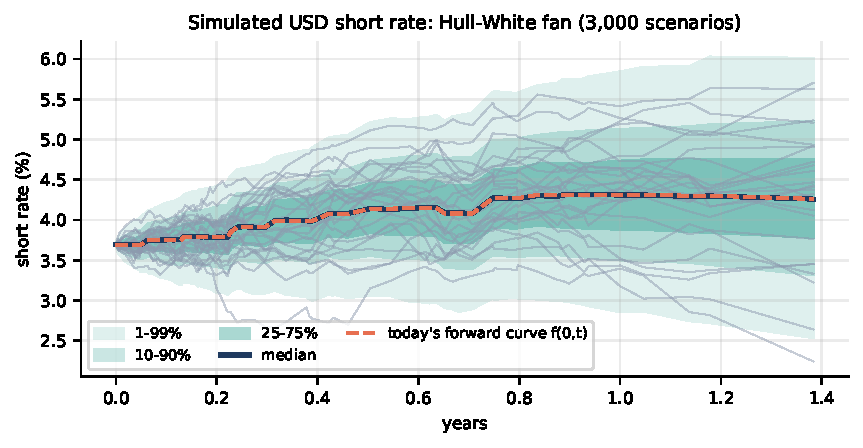
\includegraphics[width=\linewidth]{figures/fig09.pdf}
\caption{Realised yield volatility by tenor against the Hull-White implied shape for the two choices of sigma. The overnight-SOFR calibration lies well below the long-end moves; the fit tracks them.}
\end{figure}
\textbf{Choice and alternative.} Implied volatility from options would be forward-looking and is the norm for pricing, but we had no single-name options data (the Bloomberg export has only SPX/TOPIX index vols, which would need a per-name basis assumption). A 3-year realised window is a documented, reproducible proxy. Its limitation is that it is backward-looking and cannot see regime changes; the model-risk study (Section 7.9) shows how much the results move if vols are 25\% and 100\% higher.

\subsection{Correlations}
\begin{figure}[H]
\centering
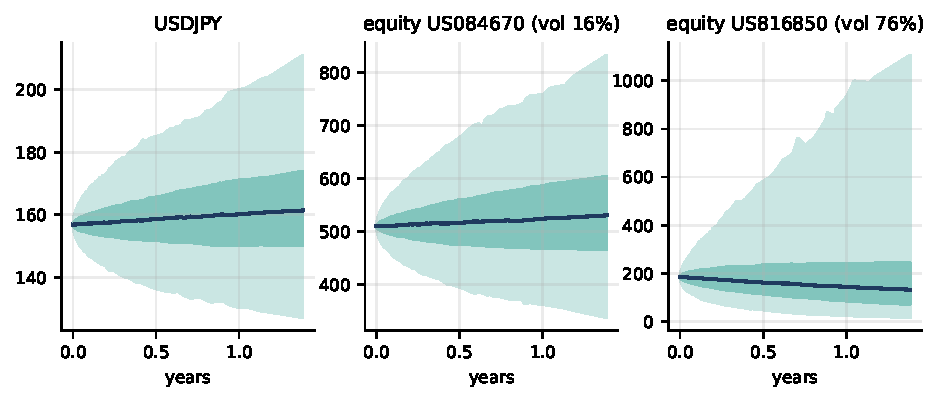
\includegraphics[width=\linewidth]{figures/fig10.pdf}
\caption{Left: the 39x39 correlation matrix reordered so similar names sit together; a broad positive `market' block is visible. Right: the 741 pairwise correlations centre on 0.14.}
\end{figure}
\textbf{Estimation and stationarity.} The matrix is static, not re-estimated per date. We take the daily returns of all 39 factors, keep only the 616 dates on which every series has a price (US and Tokyo trade on different calendars, so series are joined by calendar date rather than timestamp), and compute one pairwise correlation matrix. The USD rate factor's row uses daily changes of the 10-year Treasury yield rather than the overnight SOFR fixing, which moves in steps on Fed dates and correlates with nothing. It is assumed constant over the simulation horizon. The alternatives (time-varying DCC-GARCH, or stressed correlations) add parameters we cannot validate with our data; we flag this as a limitation.

\clearpage
\section{The risk-factor models}
\subsection{USD short rate: Hull-White one-factor}
We need the whole USD curve at every future date and scenario, because bonds and funding legs are discounted with it. The standard tool is the \textbf{Hull-White one-factor model}, a Gaussian, mean-reverting short-rate model:

{\fontsize{7.2}{8.8}\selectfont
\begin{verbatim}
dr(t) = [ theta(t) - a * r(t) ] dt + sigma dW(t)
\end{verbatim}}
\textbf{a} is mean reversion (how fast rates are pulled back), \textbf{sigma} is rate volatility, and \textbf{theta(t)} is chosen so that the model prices today's curve exactly. We use the equivalent shifted Ornstein-Uhlenbeck form r(t) = x(t) + alpha(t):

{\fontsize{7.2}{8.8}\selectfont
\begin{verbatim}
x(t+dt) = x(t) e^{-a dt} + sigma sqrt( (1 - e^{-2 a dt}) / (2a) ) Z      (exact transition)
alpha(t) = f(0,t) + sigma^2/(2 a^2) (1 - e^{-a t})^2                      (fits today's curve)
P(t,T)   = A(t,T) exp( -B(t,T) r(t) ),  B = (1 - e^{-a (T-t)})/a        (analytic bond price)
\end{verbatim}}
\textbf{Why this model.} (1) It reproduces today's curve to 1e-9 (tested). (2) Bond prices at future nodes are analytic, so building the discount curve for a scenario costs one function evaluation (10x faster than building a curve object, and exact rather than interpolated). (3) It is Gaussian, so it can produce negative rates, essential for JPY history and harmless for USD. \textbf{Alternatives rejected:} CIR/Black-Karasinski (positive-only, cannot represent negative JPY rates); LMM/HJM multi-factor curve models (more realistic curve twists but many more parameters than our data can support and slower); a constant-rate assumption (would ignore the funding-leg and bond-forward rate risk).

\textbf{Parameters.} sigma = 0.96\% (fitted to realised 2y-30y Treasury yield volatility, Section 3.2); a = 0.0167 (calibrated, Section 6). Today's short rate r(0) = 3.69\%.

\begin{figure}[H]
\centering
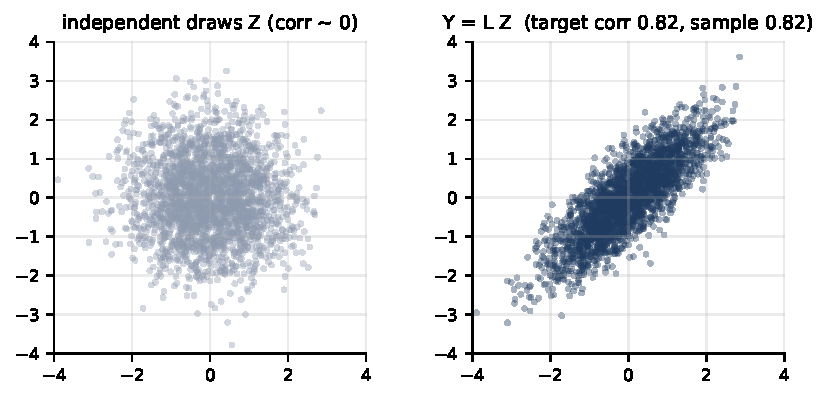
\includegraphics[width=\linewidth]{figures/fig11.pdf}
\caption{Simulated USD short rate. The median tracks today's forward curve (dashed) because the model is fitted to it; the widening bands are rate uncertainty.}
\end{figure}
\subsection{Equities and USDJPY: correlated geometric Brownian motion}
{\fontsize{7.2}{8.8}\selectfont
\begin{verbatim}
dS_i / S_i = ( r_USD - q_i ) dt + sigma_i dW_i                         USD-quoted names
dS_i / S_i = ( r_JPY - q_i + rho_iX sigma_i sigma_X ) dt + sigma_i dW_i   JPY-quoted names (S in JPY)
dX / X     = ( r_JPY - r_USD + sigma_X^2 ) dt + sigma_X dW_X             USDJPY, X = JPY per USD
\end{verbatim}}
Each step is the exact log-normal step ln S(t+dt) = ln S(t) + (drift - sigma\textasciicircum{}2/2) dt + sigma sqrt(dt) Z, with the short rates at the start of the step (so equities, FX and rates are linked). The drifts follow from requiring that every USD-denominated tradable asset, discounted at the USD money market, is a martingale. A JPY bank account valued in USD, B\_JPY / X, must earn the USD rate, which gives USDJPY (JPY per USD) a drift of r\_JPY - r\_USD: it falls when USD rates exceed JPY rates. A JPY-listed name held by a USD investor has USD value S / X and must also earn r\_USD - q, which gives the JPY-currency price the drift r\_JPY - q plus a quanto correction rho sigma\_S sigma\_X. Both are verified by martingale tests (Section 11.2). An earlier version used the drift of USD-per-JPY for a JPY-per-USD quote, with the wrong sign; the correction is documented in Section 12 and its effect in Section 7.3.

\textbf{Why GBM.} It matches the lognormal vol convention we measure, is the market default for equity CCR, and needs only a vol per name. \textbf{Alternatives:} local/stochastic vol (Heston, SABR) would capture skew and vol-of-vol but need option surfaces we do not have; jump models help tails but add unobservable parameters. We disclose that GBM understates fat tails.

\begin{figure}[H]
\centering
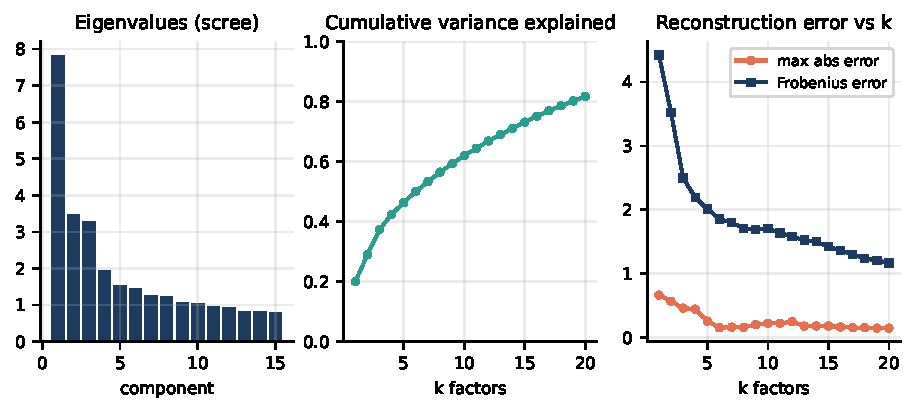
\includegraphics[width=\linewidth]{figures/fig12.pdf}
\caption{Simulated USDJPY and two equities (a low-vol and the highest-vol name) with 1-99 and 25-75 percent bands.}
\end{figure}
\subsection{Correlation and the Cholesky factor}
Independent random numbers give independent assets. Real assets move together, so we transform independent standard normals Z into correlated ones. Given the target correlation matrix C, the \textbf{Cholesky decomposition} finds the lower-triangular L with L L' = C. Then Y = L Z has exactly correlation C:

{\fontsize{7.2}{8.8}\selectfont
\begin{verbatim}
Cov(Y) = L Cov(Z) L' = L I L' = L L' = C
\end{verbatim}}
It is used because it is the cheapest exact way to impose an arbitrary positive-definite correlation structure. A tiny eigenvalue clip guards against CSV round-off making C numerically non-PSD.

\begin{figure}[H]
\centering
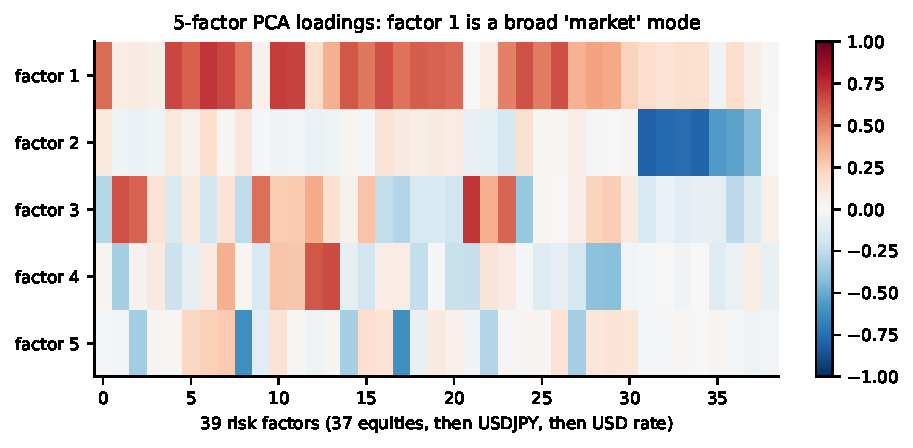
\includegraphics[width=\linewidth]{figures/fig13.pdf}
\caption{Demonstration on the most correlated pair in our real matrix (US21037T / US92840M, corr 0.82): independent draws (left) become correlated draws (right) after multiplying by L.}
\end{figure}
\subsection{Optional alternative: a PCA factor model for correlation}
A 39x39 matrix has 741 free correlations estimated from only 616 days, so many entries are noisy. A \textbf{factor model} assumes co-movement comes from a few common drivers plus each name's own noise: C $\sim$ B B' + diag(d), where B (39 x k) are loadings on k factors. We build it by principal-component analysis: B = top-k eigenvectors x sqrt(eigenvalue), and d = 1 - row sums of squares so every name still has unit variance. Simulation then draws k systematic and 39 idiosyncratic shocks.

\begin{figure}[H]
\centering
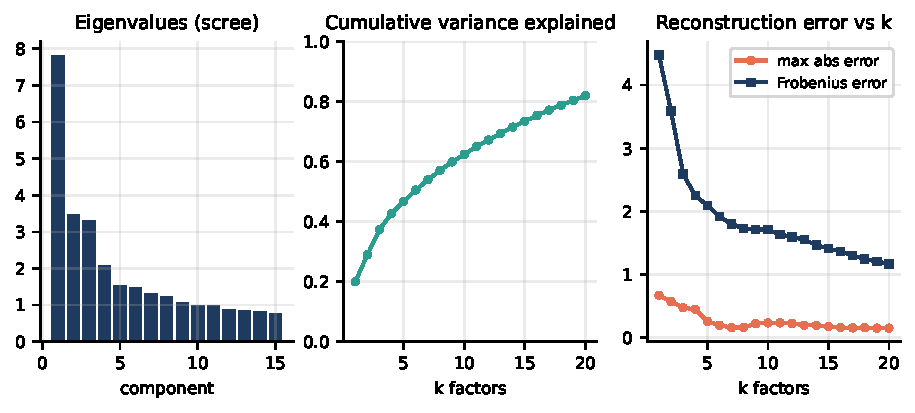
\includegraphics[width=\linewidth]{figures/fig14.pdf}
\caption{Left: the first eigenvalue (7.8 of a total 39) is one dominant market factor. Middle: 5 factors explain 47\% of variance and 10 explain 62\%. Right: reconstruction error falls as k grows (exactly zero at full rank).}
\end{figure}
\begin{figure}[H]
\centering
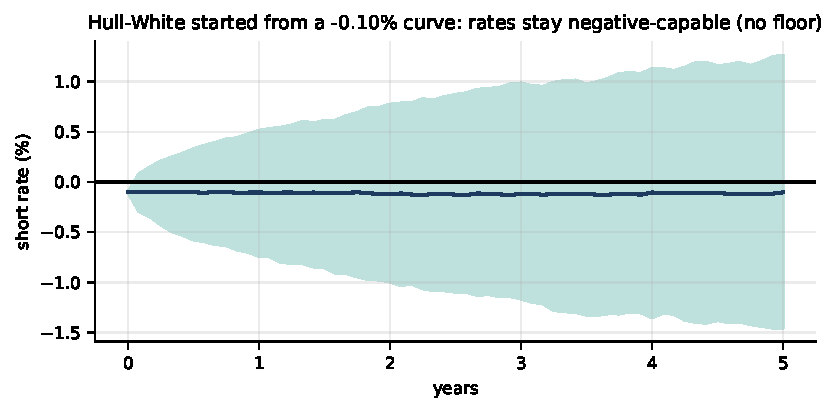
\includegraphics[width=\linewidth]{figures/fig15.pdf}
\caption{Loadings of each of the 39 factors on the first five principal factors.}
\end{figure}
\textbf{Trade-off.} The factor model is smoother and more robust to estimation noise and gives quasi-random sequences a low-dimensional space where they work best, but it only approximates the empirical matrix. Because it changes results, it is an option (corr\_mode=`factor'), not the default. Section 7.8 compares its exposure profiles with the full-rank engine.

\textbf{What the factors are.} The factors are the eigenvectors of the 39x39 correlation matrix of the 37 equities, USDJPY and the USD rate; each name's loading is its correlation with that factor. They are statistical, not economic, factors, but their loadings can be read off the data. The first factor is the market: every name loads positively and it alone explains 20\% of the variance. The later factors separate groups of names that move together.

{\scriptsize\setlength{\LTpre}{4pt}\setlength{\LTpost}{6pt}
\begin{longtable}{>{\raggedright\arraybackslash}p{\dimexpr 0.0617\linewidth-2\tabcolsep\relax}>{\raggedright\arraybackslash}p{\dimexpr 0.0988\linewidth-2\tabcolsep\relax}>{\raggedright\arraybackslash}p{\dimexpr 0.2716\linewidth-2\tabcolsep\relax}>{\raggedright\arraybackslash}p{\dimexpr 0.2716\linewidth-2\tabcolsep\relax}>{\raggedright\arraybackslash}p{\dimexpr 0.1235\linewidth-2\tabcolsep\relax}>{\raggedright\arraybackslash}p{\dimexpr 0.1728\linewidth-2\tabcolsep\relax}}
\toprule
\rowcolor{navy}\textbf{\textcolor{white}{Factor}} & \textbf{\textcolor{white}{Share of variance}} & \textbf{\textcolor{white}{Highest loadings}} & \textbf{\textcolor{white}{Lowest loadings}} & \textbf{\textcolor{white}{Mean loading, US names / JPY names}} & \textbf{\textcolor{white}{Reading}} \\
\endhead
1 & 20.0\% & NXPI +0.25, BAC +0.25, JPM +0.24, WBS +0.24 & 4503.T -0.02, KO -0.00, RATE\_USD +0.01, PM +0.02 & +0.16 / +0.04 & Market factor: all names, both regions \\
\rowcolor{gray!9}2 & 8.9\% & 6902.T +0.43, 5108.T +0.43, 7751.T +0.42, 4901.T +0.41 & NXPI -0.09, KLAC -0.07, QCOM -0.06, AMZN -0.06 & -0.01 / +0.38 & Japan versus US \\
3 & 8.5\% & KO +0.40, PG +0.35, BRK.B +0.32, PGR +0.32 & KLAC -0.21, VST -0.16, SMTC -0.16, CEG -0.14 & +0.06 / -0.06 & Defensive staples against high-growth technology and power names \\
\rowcolor{gray!9}4 & 5.3\% & MPC +0.44, XOM +0.43, RATE\_USD +0.34, WBS +0.23 & HDB -0.28, IBN -0.28, PG -0.21, HD -0.18 & -0.00 / -0.04 & Energy names and the USD rate against the Indian ADRs \\
5 & 4.0\% & CEG +0.39, NFLX +0.39, VST +0.37, PGR +0.30 & WBS -0.25, NXPI -0.22, HD -0.18, BAC -0.16 & +0.02 / -0.00 & Growth and power names against banks and semiconductors \\
\bottomrule
\end{longtable}}

{\small Tickers, signed loadings; the sign of a factor is arbitrary. Factor 2 separates the Tokyo listings from the US names; factors 3 to 5 pick out groups that move together (defensive staples, energy names together with the USD rate, and growth and power names against banks and semiconductors). Each explains only a few percent of the variance, which is why more than five factors are needed to reproduce the matrix closely.}

\textbf{What accuracy is given up, on the real book.} The one-year-horizon volatility of each netting set's equity position under the full correlation matrix and under the k-factor reconstruction (diagonal restored to one), in USD:

{\scriptsize\setlength{\LTpre}{4pt}\setlength{\LTpost}{6pt}
\begin{longtable}{>{\raggedright\arraybackslash}p{\dimexpr 0.1333\linewidth-2\tabcolsep\relax}>{\raggedright\arraybackslash}p{\dimexpr 0.2267\linewidth-2\tabcolsep\relax}>{\raggedright\arraybackslash}p{\dimexpr 0.2133\linewidth-2\tabcolsep\relax}>{\raggedright\arraybackslash}p{\dimexpr 0.2133\linewidth-2\tabcolsep\relax}>{\raggedright\arraybackslash}p{\dimexpr 0.2133\linewidth-2\tabcolsep\relax}}
\toprule
\rowcolor{navy}\textbf{\textcolor{white}{Factors k}} & \textbf{\textcolor{white}{Cumulative variance explained}} & \textbf{\textcolor{white}{Portfolio vol, CPTY\_A}} & \textbf{\textcolor{white}{Portfolio vol, CPTY\_B}} & \textbf{\textcolor{white}{Portfolio vol, CPTY\_C}} \\
\endhead
3 & 37\% & \$53.2M (+0.6\%) & \$20.0M (+2.1\%) & \$26.3M (+3.4\%) \\
\rowcolor{gray!9}5 & 47\% & \$52.9M (+0.0\%) & \$19.9M (+1.7\%) & \$26.4M (+3.9\%) \\
10 & 62\% & \$53.5M (+1.1\%) & \$19.9M (+1.5\%) & \$25.8M (+1.7\%) \\
\rowcolor{gray!9}Full matrix & 100\% & \$52.9M (reference) & \$19.6M (reference) & \$25.4M (reference) \\
\bottomrule
\end{longtable}}

\textbf{How much speed does it add?} None, and slightly the opposite. The factor model replaces a 40x40 matrix product per step with a 40x5 one plus independent noise, but the engine then has to draw k systematic and 40 idiosyncratic normals per step instead of 40, and the measured time of the correlated-shock step is not lower (full 1.91 s, 5 factors 2.08 s, 10 factors 2.29 s). In any case that step is a vanishing part of the run, which is dominated by repricing every trade at every node (2134 s for 5,000 scenarios on the close-out grid):

{\scriptsize\setlength{\LTpre}{4pt}\setlength{\LTpost}{6pt}
\begin{longtable}{>{\raggedright\arraybackslash}p{\dimexpr 0.2162\linewidth-2\tabcolsep\relax}>{\raggedright\arraybackslash}p{\dimexpr 0.2162\linewidth-2\tabcolsep\relax}>{\raggedright\arraybackslash}p{\dimexpr 0.3514\linewidth-2\tabcolsep\relax}>{\raggedright\arraybackslash}p{\dimexpr 0.2162\linewidth-2\tabcolsep\relax}}
\toprule
\rowcolor{navy}\textbf{\textcolor{white}{Corr. mode}} & \textbf{\textcolor{white}{Random factors per step}} & \textbf{\textcolor{white}{Correlated-shock step (5,000 scenarios)}} & \textbf{\textcolor{white}{Share of the reporting run}} \\
\endhead
Full Cholesky & 40 & 1.91 s & 0.089\% \\
\rowcolor{gray!9}PCA, 5 factors & 45 & 2.08 s & 0.097\% \\
PCA, 10 factors & 50 & 2.29 s & 0.107\% \\
\bottomrule
\end{longtable}}

The correlated-shock step is 1.91 s (full) against 2.08 s (5 factors) in a run of 2134 s, so the end-to-end speed added is nil; whichever is faster, the difference is under 0.1\% of the run.

\textbf{Does it help the sampling error?} The hope for a factor model with quasi-random numbers is a lower-dimensional space. Here the engine draws the five systematic and the 40 idiosyncratic shocks with the same Latin Hypercube generator, so the dimension per step rises from 40 to 45. Measured on the one-month PFE99 of each netting set's equity positions over 10 seeds at N = 1000, against a pseudo-random full-rank reference at N = 10,000:

{\scriptsize\setlength{\LTpre}{4pt}\setlength{\LTpost}{6pt}
\begin{longtable}{>{\raggedright\arraybackslash}p{\dimexpr 0.2105\linewidth-2\tabcolsep\relax}>{\raggedright\arraybackslash}p{\dimexpr 0.1316\linewidth-2\tabcolsep\relax}>{\raggedright\arraybackslash}p{\dimexpr 0.1316\linewidth-2\tabcolsep\relax}>{\raggedright\arraybackslash}p{\dimexpr 0.1316\linewidth-2\tabcolsep\relax}>{\raggedright\arraybackslash}p{\dimexpr 0.1316\linewidth-2\tabcolsep\relax}>{\raggedright\arraybackslash}p{\dimexpr 0.1316\linewidth-2\tabcolsep\relax}>{\raggedright\arraybackslash}p{\dimexpr 0.1316\linewidth-2\tabcolsep\relax}}
\toprule
\rowcolor{navy}\textbf{\textcolor{white}{Corr. mode}} & \textbf{\textcolor{white}{Std of PFE99, CPTY\_A (\% of reference)}} & \textbf{\textcolor{white}{Std of PFE99, CPTY\_B (\% of reference)}} & \textbf{\textcolor{white}{Std of PFE99, CPTY\_C (\% of reference)}} & \textbf{\textcolor{white}{Bias, CPTY\_A (\% of reference)}} & \textbf{\textcolor{white}{Bias, CPTY\_B (\% of reference)}} & \textbf{\textcolor{white}{Bias, CPTY\_C (\% of reference)}} \\
\endhead
Full Cholesky & 4.5\% & 4.5\% & 4.9\% & +2.7\% & +1.2\% & +1.8\% \\
\rowcolor{gray!9}PCA, 3 factors & 4.0\% & 6.2\% & 5.0\% & +0.3\% & +1.5\% & +6.1\% \\
PCA, 5 factors & 4.9\% & 3.3\% & 4.1\% & +4.7\% & -1.0\% & +9.1\% \\
\rowcolor{gray!9}PCA, 10 factors & 4.5\% & 3.8\% & 2.6\% & +1.1\% & +0.6\% & +2.5\% \\
\bottomrule
\end{longtable}}

\begin{center}\fcolorbox{teal}{teal!7}{\parbox{0.94\linewidth}{\vspace{2pt}Conclusion: the PCA factor model is explainable (a market factor, a Japan-versus-US factor and group factors) but it approximates the correlation matrix (the volatility of a netting set differs from the full matrix by several percent), it adds no speed, and its sampling error is not consistently lower than the full-rank model's (it varies with the number of factors and the netting set). The full-rank Cholesky remains the default; the factor model is kept as a robustness option, and would become useful only if the systematic factors alone were drawn quasi-randomly and the idiosyncratic noise pseudo-randomly.\vspace{2pt}}}\end{center}
\clearpage
\subsection{JPY: a negative-rate-capable rate model}
Until recently JPY drift used r\_USD minus a constant differential. That cannot represent JPY's own rate dynamics. We therefore built a genuine second Hull-White factor for JPY (\texttt{build\_jpy\_hull\_white}): it starts from the real JPY OIS curve and, being Gaussian, has \textbf{no floor at zero}.

\begin{figure}[H]
\centering
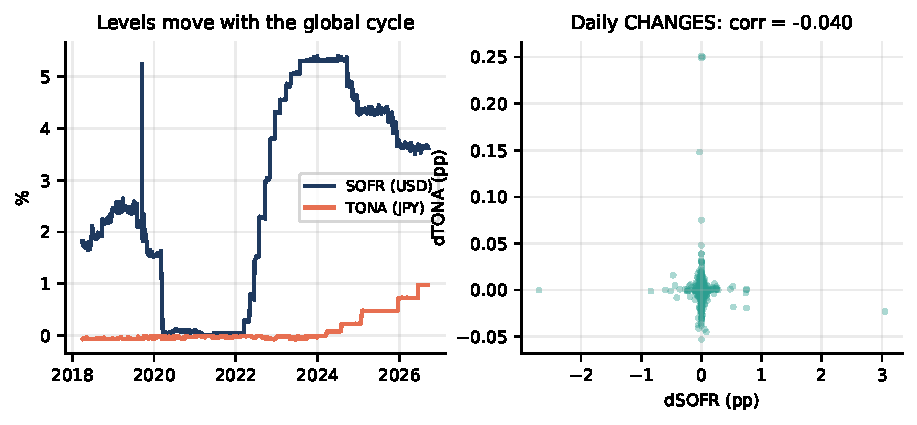
\includegraphics[width=\linewidth]{figures/fig16.pdf}
\caption{Real TONA history from the Bank of Japan: rates were at or below zero for most of 25 years, with 1995 negative daily fixings (2003 and 2016-2024). A model that floors at zero could not represent this.}
\end{figure}
The daily JPY OIS history provided by the project team (35 tenors, 3903 business days from October 2011) shows the same for the whole short end of the curve: the overnight call rate was negative on 2109 days, and OIS par rates out to five years were negative on 2340 days, with a minimum of -0.37\%.

\begin{figure}[H]
\centering
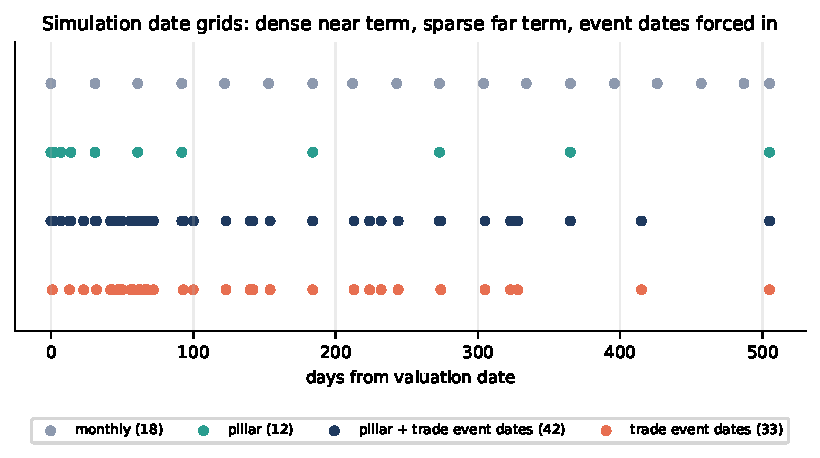
\includegraphics[width=\linewidth]{figures/fig17.pdf}
\caption{Demonstration of the capability: Hull-White started from a synthetic -0.10\% flat curve. 63\% of simulated points are negative and nothing is clipped. (Our only real JPY curve snapshot, Aug 2026, is positive after BOJ hikes, so the negative case is shown synthetically.)}
\end{figure}
{\footnotesize\setlength{\LTpre}{4pt}\setlength{\LTpost}{6pt}
\begin{longtable}{>{\raggedright\arraybackslash}p{\dimexpr 0.2338\linewidth-2\tabcolsep\relax}>{\raggedright\arraybackslash}p{\dimexpr 0.2078\linewidth-2\tabcolsep\relax}>{\raggedright\arraybackslash}p{\dimexpr 0.5584\linewidth-2\tabcolsep\relax}}
\toprule
\rowcolor{navy}\textbf{\textcolor{white}{JPY factor parameter}} & \textbf{\textcolor{white}{Value}} & \textbf{\textcolor{white}{Source / status}} \\
\endhead
Curve & JPY OIS zero curve, 2026-08-28 & Bootstrapped from the daily JPY OIS par history (project-team Bloomberg file); matches Bloomberg's own zero curve to within 1bp at all tenors \\
\rowcolor{gray!9}sigma & 0.267\%/yr & Realised vol of the overnight call rate, 3y window, from the same OIS file (Bank of Japan TONA gives 0.276\%, consistent) \\
a (mean reversion) & 0.0010 & Lower bound: all three real JPY calibrations gave a negative a (Section 6.2) \\
\rowcolor{gray!9}USD-JPY rate-factor correlation & -0.040 & Calibrated from real SOFR vs TONA daily changes (n=1983, p=0.07): statistically zero \\
Correlation with USDJPY and the equities & USDJPY +0.04; equities -0.04 to +0.21 & Daily changes of the 1-year JPY OIS rate against daily returns, same 3-year window (n=778) \\
\rowcolor{gray!9}Wired into simulate\_paths()? & YES & The simulated JPY rate drives the drift of the JPY-listed names and USDJPY, and a JPY discount curve is available at every node \\
\bottomrule
\end{longtable}}

\begin{figure}[H]
\centering
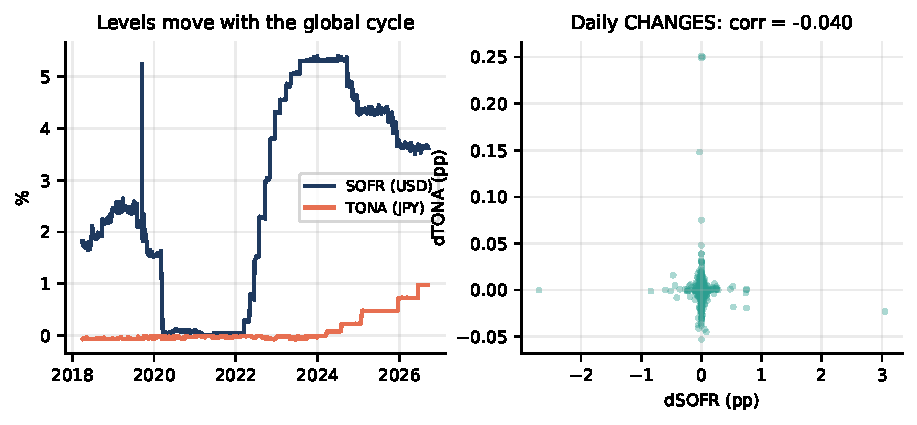
\includegraphics[width=\linewidth]{figures/fig18.pdf}
\caption{Levels (left) rise together with the global cycle (level correlation $\sim$0.38), but day-to-day changes (right) are uncorrelated (-0.040): central banks set policy independently. A Hull-White correlation needs the CHANGES.}
\end{figure}
\textbf{Effect on the results.} Only 2 of 16 trades hold JPY names, so the effect is confined to their netting sets; its size, together with that of the USDJPY drift correction, is measured in the attribution of Section 7.3.

\subsection{A two-factor rates model: G2++}
The one-factor model moves every zero rate in lock-step with the short rate. A richer alternative is a two-factor Gaussian model (G2++, equivalent to a two-factor LGM): r(t) = x(t) + y(t) + phi(t), with dx = -a x dt + sigma dW1, dy = -b y dt + eta dW2 and correlation rho, which allows the curve to change slope independently of its level. It keeps the Gaussian properties that matter here (analytic bond prices at every node, negative rates possible) and fits today's curve exactly. It is implemented in models/g2pp.py and selected with rates\_model=`g2pp'; the second factor is driven by rho times the first factor's shock plus an extra independent shock, so it inherits the first factor's correlations with equities and FX.

Calibration is to the realised covariance of daily changes of the 3-month to 30-year Treasury yields (3-year window), least squares on the whole covariance matrix, so both the volatility level by tenor and the correlation between tenors are matched: sigma = 1.21\%, a = 0.039, eta = 1.44\%, b = 1.50, rho = -0.95, with a relative Frobenius error of 16\%. The fit reproduces the level and slope of the volatility term structure but not the hump around the 5-year point, which no two-factor Gaussian model can produce.

\begin{figure}[H]
\centering
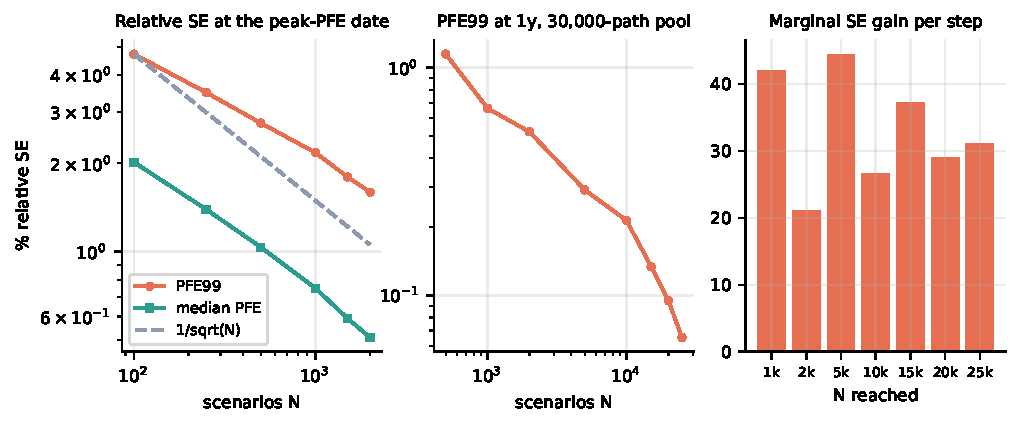
\includegraphics[width=\linewidth]{figures/fig19.pdf}
\caption{Realised yield-change volatility by tenor against the fitted two-factor model.}
\end{figure}
{\scriptsize\setlength{\LTpre}{4pt}\setlength{\LTpost}{6pt}
\begin{longtable}{>{\raggedright\arraybackslash}p{\dimexpr 0.1667\linewidth-2\tabcolsep\relax}>{\raggedright\arraybackslash}p{\dimexpr 0.1795\linewidth-2\tabcolsep\relax}>{\raggedright\arraybackslash}p{\dimexpr 0.1795\linewidth-2\tabcolsep\relax}>{\raggedright\arraybackslash}p{\dimexpr 0.1154\linewidth-2\tabcolsep\relax}>{\raggedright\arraybackslash}p{\dimexpr 0.1795\linewidth-2\tabcolsep\relax}>{\raggedright\arraybackslash}p{\dimexpr 0.1795\linewidth-2\tabcolsep\relax}}
\toprule
\rowcolor{navy}\textbf{\textcolor{white}{Netting set}} & \textbf{\textcolor{white}{MPE99, one factor}} & \textbf{\textcolor{white}{MPE99, two factors}} & \textbf{\textcolor{white}{Change}} & \textbf{\textcolor{white}{Peak EE, one factor}} & \textbf{\textcolor{white}{Peak EE, two factors}} \\
\endhead
CPTY\_A & \$26.2M & \$26.0M & -1\% & \$4.7M & \$4.6M \\
\rowcolor{gray!9}CPTY\_B & \$9.5M & \$9.3M & -3\% & \$1.8M & \$1.8M \\
CPTY\_C & \$28.9M & \$28.9M & -0\% & \$5.2M & \$5.0M \\
\rowcolor{gray!9}Portfolio & \$51.5M & \$50.0M & -3\% & \$11.6M & \$11.4M \\
\bottomrule
\end{longtable}}

{\small Close-out exposure within one year, 2,000 scenarios, same random numbers.}

\clearpage
\section{How the simulation engine works}
\subsection{The pipeline}
{\fontsize{7.2}{8.8}\selectfont
\begin{verbatim}
1. calibrate:   curve (futures + long end), sigma, a, JPY factor, vols, corr (real data)
2. grid:        pillar dates + trade event dates + t-1bd and t+10bd nodes around every reporting date
3. draw:        random numbers (Latin Hypercube) -> correlated shocks (Cholesky or PCA)
4.  step:       advance USD and JPY short rates, 37 equities, USDJPY along every path
5. reprice:     for every (scenario, node): build MarketState, call npv() of all 16 trades
6. aggregate:   max(V(t+10bd) - V(t-1bd), 0), netted by counterparty -> EE, median PFE, PFE99, MPE
\end{verbatim}}
\subsection{Choosing the simulation dates}
Monthly steps are simple but wasteful and blunt: they spend nodes evenly when the risk changes fastest near term, and a trade's own reset or maturity rarely falls on a month node. Following Capitolis' guidance, we adopt \textbf{pillar dates}: the standard market curve tenors also used to build the SOFR curve (O/N, T/N, 1W, 2W, 1M, 2M, 3M, 6M, 9M, 1Y, 18M, 2Y ...). This mirrors production CCR practice: dense short-term, sparse long-term. In addition, every trade's own reset/settlement/maturity date is \textbf{forced onto the grid} so exposure jumps at cash-flow dates are not smoothed over.

\begin{figure}[H]
\centering
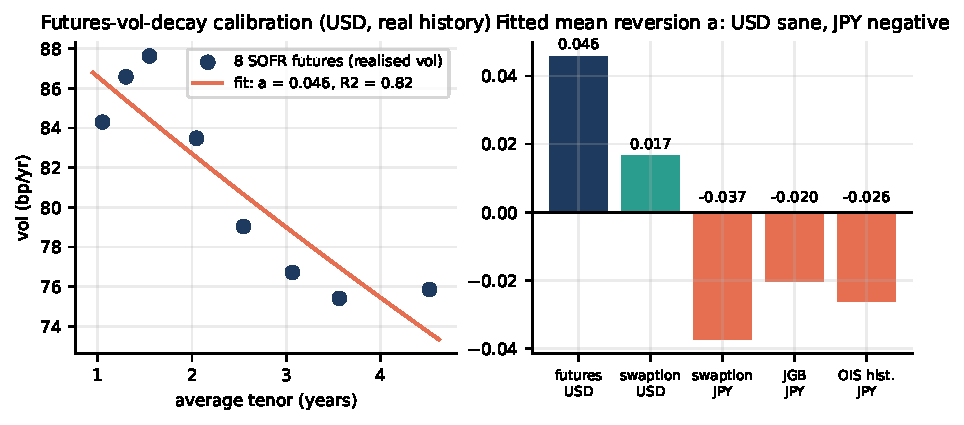
\includegraphics[width=\linewidth]{figures/fig20.pdf}
\caption{For this book the pillar grid (12 dates) plus forced trade-event dates (42 in total) is more compact than a plain monthly grid (18) and hits every real cash-flow date exactly.}
\end{figure}
\subsection{Speed}
{\footnotesize\setlength{\LTpre}{4pt}\setlength{\LTpost}{6pt}
\begin{longtable}{>{\raggedright\arraybackslash}p{\dimexpr 0.2469\linewidth-2\tabcolsep\relax}>{\raggedright\arraybackslash}p{\dimexpr 0.3951\linewidth-2\tabcolsep\relax}>{\raggedright\arraybackslash}p{\dimexpr 0.1481\linewidth-2\tabcolsep\relax}>{\raggedright\arraybackslash}p{\dimexpr 0.2099\linewidth-2\tabcolsep\relax}}
\toprule
\rowcolor{navy}\textbf{\textcolor{white}{Bottleneck}} & \textbf{\textcolor{white}{Fix}} & \textbf{\textcolor{white}{Before}} & \textbf{\textcolor{white}{After}} \\
\endhead
Discount curve per (scenario, node) & Analytic Hull-White bond price instead of building a Curve object & 0.206 ms/call & 0.019 ms/call (10.6x, and exact) \\
\rowcolor{gray!9}Pure-Python pricers ($\sim$1.2 ms each) & Multiprocessing over scenarios, 8 workers (a Windows spawn re-import bug was fixed) & 113 ms/scenario & 51 ms/scenario at the time \\
Combined, 2,000 scenarios x 16 trades &  & $\sim$12 min projected & 93 s (7.7x) \\
\bottomrule
\end{longtable}}

Current measured cost for the 3,000-scenario reporting run: 1 s simulation of paths, 3576 s repricing (1192 ms/scenario, including the extra MPOR look-ahead nodes).

\subsection{Random numbers and variance reduction}
Plain pseudo-random draws waste information: by chance a sample can cluster. Five sampling schemes sit behind one interface: \textbf{pseudo-random} (baseline), \textbf{antithetic} (each draw z paired with -z), \textbf{moment-matched} (rescale so the sample mean is 0 and std 1), \textbf{Sobol} (low-discrepancy quasi-random), and \textbf{Latin Hypercube} (each dimension split into equal-probability bins, one draw per bin).

\begin{figure}[H]
\centering
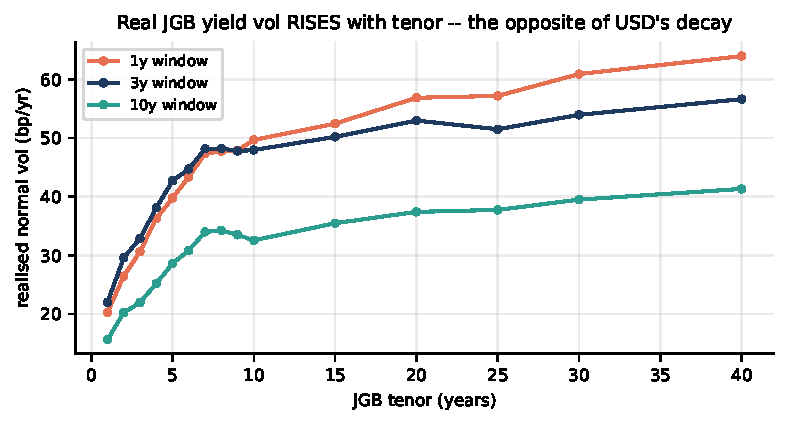
\includegraphics[width=\linewidth]{figures/fig21.pdf}
\caption{Left: on a European call with a known Black-Scholes value, Latin Hypercube has about 51x lower error than pseudo-random. Right: on the real 663-dimensional engine (300 scenarios, 8 repeats) the methods are much closer, and no method is best for both PFE99 and the median PFE.}
\end{figure}
{\footnotesize\setlength{\LTpre}{4pt}\setlength{\LTpost}{6pt}
\begin{longtable}{>{\raggedright\arraybackslash}p{\dimexpr 0.1348\linewidth-2\tabcolsep\relax}>{\raggedright\arraybackslash}p{\dimexpr 0.0899\linewidth-2\tabcolsep\relax}>{\raggedright\arraybackslash}p{\dimexpr 0.1124\linewidth-2\tabcolsep\relax}>{\raggedright\arraybackslash}p{\dimexpr 0.1573\linewidth-2\tabcolsep\relax}>{\raggedright\arraybackslash}p{\dimexpr 0.1685\linewidth-2\tabcolsep\relax}>{\raggedright\arraybackslash}p{\dimexpr 0.3371\linewidth-2\tabcolsep\relax}}
\toprule
\rowcolor{navy}\textbf{\textcolor{white}{Method}} & \textbf{\textcolor{white}{Call RMSE}} & \textbf{\textcolor{white}{vs pseudo-random}} & \textbf{\textcolor{white}{PFE99 rel. std (real engine)}} & \textbf{\textcolor{white}{Median PFE rel. std (real engine)}} & \textbf{\textcolor{white}{Verdict}} \\
\endhead
pseudo random & 1.4563 & - & 2.60\% (1.00x) & 0.66\% (1.00x) & Baseline \\
\rowcolor{gray!9}antithetic & 1.0786 & 1.4x better & 1.98\% (1.31x) & 0.39\% (1.69x) & Improves both measures modestly on the real engine, but only 1.4x on the controlled test \\
moment matched & 0.2317 & 6.3x better & 2.49\% (1.04x) & 0.35\% (1.91x) & Helps the median only; no PFE99 benefit \\
\rowcolor{gray!9}sobol & 0.0507 & 28.7x better & 1.64\% (1.58x) & 0.70\% (0.95x) & Best PFE99 on the real engine but no median benefit; unscrambled Sobol degrades in high dimension and is harder to replicate \\
latin hypercube & 0.0288 & 50.6x better & 2.25\% (1.15x) & 0.42\% (1.57x) & SELECTED: 50x on the controlled test and improves both PFE99 and median PFE on the real engine \\
\bottomrule
\end{longtable}}

{\small Relative standard deviation of the estimator across 8 independent repeats at 300 scenarios (portfolio, about 6 weeks out, near the PFE99 peak); the multiple in brackets is the improvement over pseudo-random. With only 8 repeats each standard deviation is itself uncertain by roughly a quarter, so real-engine differences between the better methods are indicative rather than conclusive.}

\textbf{Finding.} The controlled test gives a clear ordering (Latin Hypercube, Sobol, moment matching, antithetic, pseudo-random). On the real engine, at 663 effective dimensions (39 factors x 17 time steps), the advantages compress and the ranking depends on the statistic: the tail (PFE99) and the centre (median PFE) respond to different methods. Latin Hypercube is the only method that is both best on the controlled test and better than pseudo-random on both real-engine statistics.

\begin{center}\fcolorbox{teal}{teal!7}{\parbox{0.94\linewidth}{\vspace{2pt}\textbf{Decision: Latin Hypercube sampling.} It is the best method on the controlled test and the most consistent across both reported statistics on the real engine, at negligible additional cost over plain pseudo-random draws. Sobol is the runner-up on the controlled test but is not recommended here because its benefit disappears for the median PFE and it is less robust at this dimensionality.\vspace{2pt}}}\end{center}
\clearpage
\subsection{Number of scenarios}
Monte Carlo error falls as 1/sqrt(N). Rather than rerun the expensive repricing at every candidate N, we estimate the standard error by bootstrap resampling of a simulated pool. Two studies are combined: (i) resampling of the 3,000-scenario reporting run, at the date of peak PFE99, for both PFE99 and the median PFE; (ii) a dedicated 30,000-scenario pool for the 99th percentile at the one-year node, which extends the range to large N.

\begin{figure}[H]
\centering
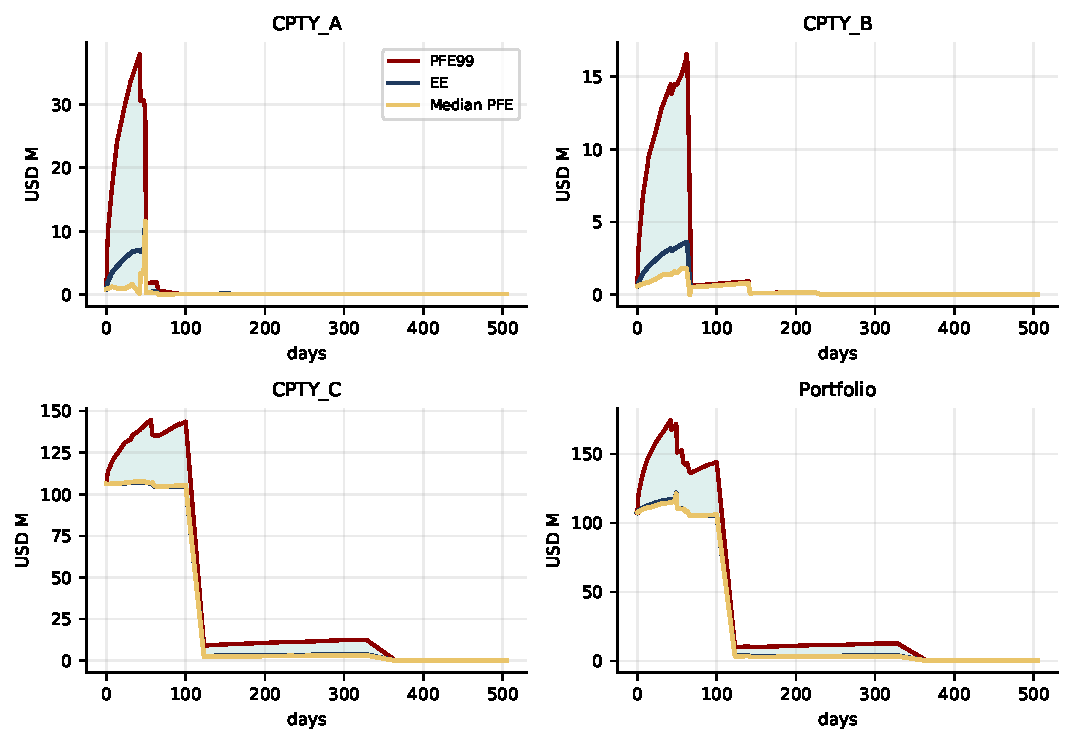
\includegraphics[width=\linewidth]{figures/fig22.pdf}
\caption{Left: relative standard error of PFE99 and median PFE at the peak-PFE date (2026-10-09); the error follows the 1/sqrt(N) law. Middle and right: PFE99 tail study at one year; error is larger for the same N, and the marginal gain per additional batch peaks at N = 5,000 and then declines.}
\end{figure}
{\footnotesize\setlength{\LTpre}{4pt}\setlength{\LTpost}{6pt}
\begin{longtable}{>{\raggedright\arraybackslash}p{\dimexpr 0.2000\linewidth-2\tabcolsep\relax}>{\raggedright\arraybackslash}p{\dimexpr 0.4000\linewidth-2\tabcolsep\relax}>{\raggedright\arraybackslash}p{\dimexpr 0.4000\linewidth-2\tabcolsep\relax}}
\toprule
\rowcolor{navy}\textbf{\textcolor{white}{N}} & \textbf{\textcolor{white}{Relative SE of PFE99}} & \textbf{\textcolor{white}{Relative SE of median PFE}} \\
\endhead
100 & 4.98\% & 2.53\% \\
\rowcolor{gray!9}250 & 2.93\% & 1.60\% \\
500 & 2.19\% & 1.16\% \\
\rowcolor{gray!9}1,000 & 1.52\% & 0.84\% \\
1,500 & 1.44\% & 0.71\% \\
\rowcolor{gray!9}2,000 & 1.41\% & 0.59\% \\
\bottomrule
\end{longtable}}

{\small Relative standard errors at the peak-PFE date, bootstrapped from the reporting run (finite-pool corrected). Extrapolating with the 1/sqrt(N) law, the 3,000-scenario run used for this report has a PFE99 relative standard error of about 0.99\% at its peak.}

{\footnotesize\setlength{\LTpre}{4pt}\setlength{\LTpost}{6pt}
\begin{longtable}{>{\raggedright\arraybackslash}p{\dimexpr 0.0875\linewidth-2\tabcolsep\relax}>{\raggedright\arraybackslash}p{\dimexpr 0.1375\linewidth-2\tabcolsep\relax}>{\raggedright\arraybackslash}p{\dimexpr 0.1125\linewidth-2\tabcolsep\relax}>{\raggedright\arraybackslash}p{\dimexpr 0.1625\linewidth-2\tabcolsep\relax}>{\raggedright\arraybackslash}p{\dimexpr 0.1375\linewidth-2\tabcolsep\relax}>{\raggedright\arraybackslash}p{\dimexpr 0.1000\linewidth-2\tabcolsep\relax}>{\raggedright\arraybackslash}p{\dimexpr 0.2625\linewidth-2\tabcolsep\relax}}
\toprule
\rowcolor{navy}\textbf{\textcolor{white}{N}} & \textbf{\textcolor{white}{PFE99 at 1y (USD)}} & \textbf{\textcolor{white}{Rel. SE at 1y}} & \textbf{\textcolor{white}{Rel. SE at peak date (est.)}} & \textbf{\textcolor{white}{Marginal SE gain (1y)}} & \textbf{\textcolor{white}{Est. time}} & \textbf{\textcolor{white}{Verdict}} \\
\endhead
500 & 149,036 & 1.15\% & 2.41\% & - & 74s & Screening only \\
\rowcolor{gray!9}1,000 & 149,353 & 0.66\% & 1.71\% & +42.1\% & 119s & Iteration and what-if runs \\
2,000 & 149,341 & 0.52\% & 1.21\% & +21.2\% & 209s & Acceptable for routine monitoring \\
\rowcolor{gray!9}5,000 & 149,457 & 0.29\% & 0.76\% & +44.4\% & 479s & RECOMMENDED: standard reporting \\
10,000 & 149,411 & 0.21\% & 0.54\% & +26.6\% & 929s & Recommended for limit sign-off \\
\rowcolor{gray!9}15,000 & 149,477 & 0.13\% & 0.44\% & +37.3\% & 1,379s & Diminishing returns \\
20,000 & 149,535 & 0.09\% & 0.38\% & +29.1\% & 1,829s & Diminishing returns \\
\rowcolor{gray!9}25,000 & 149,505 & 0.07\% & 0.34\% & +31.1\% & 2,279s & Diminishing returns \\
\bottomrule
\end{longtable}}

{\small Tail study at the one-year node (pool value \$149,482, 30,000 scenarios) and the corresponding estimate at the date of peak PFE99, where the exposure distribution is wider (relative SE = 1.7\% / sqrt(N/1000), fitted to the reporting-run bootstrap). Times assume 8 cores.}

\begin{center}\fcolorbox{teal}{teal!7}{\parbox{0.94\linewidth}{\vspace{2pt}\textbf{Decision: number of paths.} Use \textbf{N = 5,000} for standard PFE99 reporting: relative standard error 0.8\% at the worst-case date (0.29\% at the one-year node), about 8 minutes on 8 cores. Use \textbf{N = 1,000} for iteration and what-if runs (1.7\% at the worst-case date, about 2 minutes) and \textbf{N = 10,000} when a limit is being signed off (0.5\%, about 15 minutes). We do not recommend more than 15,000: cost grows linearly while error falls only as 1/sqrt(N), and the remaining sampling error (below 0.4\%) is an order of magnitude smaller than the model sensitivities in Section 7.9 (a 25\% increase in equity volatility moves the portfolio MPE by about 19\%). These figures are for the uncollateralized level exposure of the earlier calibration; the level figures of this report use N = 3,000 (1.0\% at the worst-case date) and the close-out headline figures N = 5,000 (bootstrap below).\vspace{2pt}}}\end{center}
\textbf{Convergence of the close-out measures.} The study above concerns the level exposure of the earlier calibration. The same bootstrap on the 5,000-scenario close-out run (subsets drawn without replacement, corrected for the finite pool) gives the relative standard error of the PFE99 at the date of the portfolio peak (2026-09-20) and of the MPE itself, shown as PFE99 / MPE:

{\scriptsize\setlength{\LTpre}{4pt}\setlength{\LTpost}{6pt}
\begin{longtable}{>{\raggedright\arraybackslash}p{\dimexpr 0.1892\linewidth-2\tabcolsep\relax}>{\raggedright\arraybackslash}p{\dimexpr 0.1622\linewidth-2\tabcolsep\relax}>{\raggedright\arraybackslash}p{\dimexpr 0.1622\linewidth-2\tabcolsep\relax}>{\raggedright\arraybackslash}p{\dimexpr 0.1622\linewidth-2\tabcolsep\relax}>{\raggedright\arraybackslash}p{\dimexpr 0.1622\linewidth-2\tabcolsep\relax}>{\raggedright\arraybackslash}p{\dimexpr 0.1622\linewidth-2\tabcolsep\relax}}
\toprule
\rowcolor{navy}\textbf{\textcolor{white}{Netting set}} & \textbf{\textcolor{white}{N = 250}} & \textbf{\textcolor{white}{N = 500}} & \textbf{\textcolor{white}{N = 1,000}} & \textbf{\textcolor{white}{N = 2,000}} & \textbf{\textcolor{white}{N = 3,000}} \\
\endhead
CPTY\_A & 7.9\% / 6.3\% & 6.5\% / 5.1\% & 4.0\% / 3.2\% & 3.2\% / 2.6\% & 3.2\% / 2.5\% \\
\rowcolor{gray!9}CPTY\_B & 8.0\% / 5.1\% & 6.3\% / 4.7\% & 4.6\% / 3.7\% & 4.3\% / 3.5\% & 3.8\% / 3.5\% \\
CPTY\_C & 10.4\% / 5.9\% & 7.5\% / 4.8\% & 5.4\% / 3.8\% & 3.1\% / 3.1\% & 2.5\% / 3.1\% \\
\rowcolor{gray!9}Portfolio & 8.3\% / 7.1\% & 6.4\% / 4.9\% & 4.4\% / 3.3\% & 2.7\% / 2.2\% & 2.6\% / 2.2\% \\
\bottomrule
\end{longtable}}

On this definition the MPE99 of the portfolio has a relative standard error of about 2.2\% at N = 2,000, which extrapolates by the 1/sqrt(N) law to about 1.4\% at N = 5,000 and 1.0\% at N = 10,000. The close-out exposure is the tail of a 10-day move of a margined position, so it is noisier per scenario than the level exposure; the recommended counts are unchanged, but the precision to quote for the headline MPE at N = 5,000 is roughly 1.4\%.

\clearpage
\section{Calibrating Hull-White mean reversion}
Mean reversion a controls how fast rate shocks decay; the convergence study flagged it as the largest unquantified model uncertainty. The textbook method is to fit swaption volatilities. Hull-White predicts that the volatility of a forward rate at maturity T decays with time to maturity:

{\fontsize{7.2}{8.8}\selectfont
\begin{verbatim}
sigma_f(t, T) = sigma * exp( -a (T - t) )      =>   ln(vol) = ln(sigma) - a * tenor   (line, slope = -a)
\end{verbatim}}
So measuring vol at several tenors and regressing ln(vol) on tenor gives a. We tried three real data routes, in order of preference:

\begin{figure}[H]
\centering
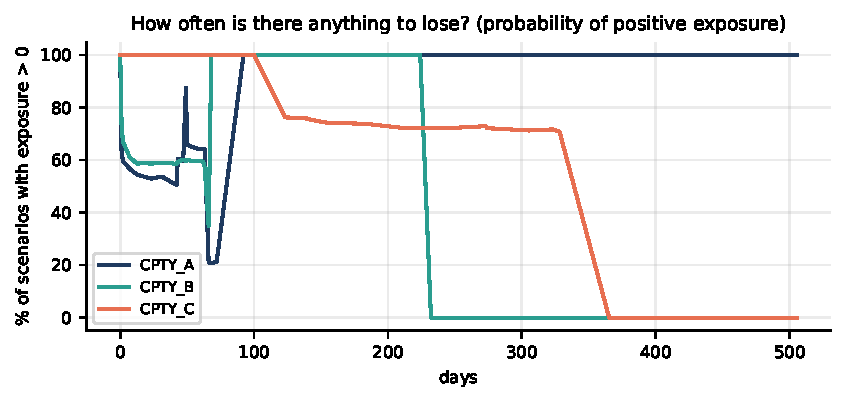
\includegraphics[width=\linewidth]{figures/fig23.pdf}
\caption{Left: USD SOFR-futures fit. Right: fitted a for each route. USD routes give sensible positive values; all three JPY routes give a NEGATIVE a.}
\end{figure}
{\footnotesize\setlength{\LTpre}{4pt}\setlength{\LTpost}{6pt}
\begin{longtable}{>{\raggedright\arraybackslash}p{\dimexpr 0.2500\linewidth-2\tabcolsep\relax}>{\raggedright\arraybackslash}p{\dimexpr 0.3250\linewidth-2\tabcolsep\relax}>{\raggedright\arraybackslash}p{\dimexpr 0.1000\linewidth-2\tabcolsep\relax}>{\raggedright\arraybackslash}p{\dimexpr 0.0750\linewidth-2\tabcolsep\relax}>{\raggedright\arraybackslash}p{\dimexpr 0.2500\linewidth-2\tabcolsep\relax}}
\toprule
\rowcolor{navy}\textbf{\textcolor{white}{Route}} & \textbf{\textcolor{white}{Data}} & \textbf{\textcolor{white}{a}} & \textbf{\textcolor{white}{R2}} & \textbf{\textcolor{white}{Verdict}} \\
\endhead
Swaption cube, USD (preferred) & Bloomberg ATM normal vol, 1M expiry, tenors 1Y-15Y & 0.0167 & 0.84 & USED for USD \\
\rowcolor{gray!9}SOFR-futures vol decay, USD & 8 contracts, $\sim$2y Databento history & 0.0458 & 0.82 & cross-check (different instrument, higher a) \\
Swaption cube, JPY & Bloomberg JPY OIS ATM vols (one snapshot) & -0.0374 & 0.84 & invalid (vol rises with tenor) \\
\rowcolor{gray!9}JGB yield vol, JPY & MOF daily 1Y-30Y yields, 3y window & -0.0203 & 0.49 & invalid (vol rises with tenor) \\
JPY OIS history, JPY (most complete) & Daily OIS par rates, 35 tenors, 2011-2026, 1Y-30Y vols, 3y window & -0.0261 & 0.62 & invalid (vol rises with tenor); lower bound a = 0.001 used \\
\bottomrule
\end{longtable}}

\subsection{Why the two USD numbers differ}
0.0167 (swaptions) versus 0.0458 (futures) is not a contradiction: they use different instruments (swaption-implied vs realised vol) and different tenor ranges (1-15Y swap tenors vs 1-3Y forward reset times). The swaption route is the industry standard and is used; the gap is itself a measure of model uncertainty and motivates the sensitivity test.

\subsection{Why JPY does not fit, and what we did}
\begin{figure}[H]
\centering
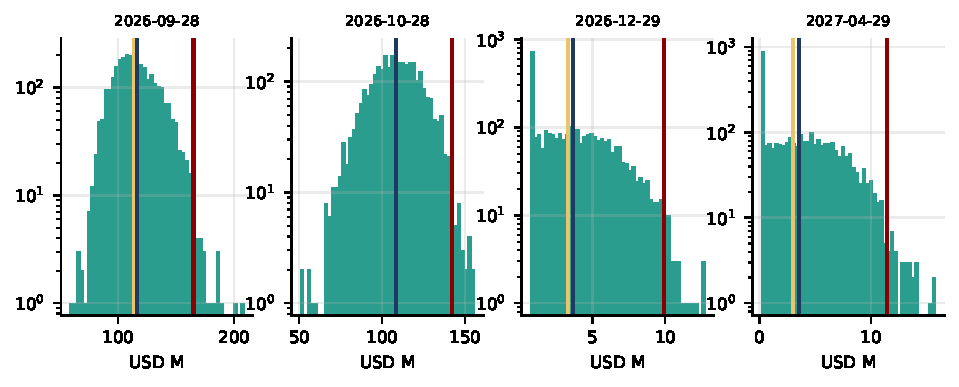
\includegraphics[width=\linewidth]{figures/fig24.pdf}
\caption{Realised volatility of JPY rates by tenor from two independent real datasets. At every window tried (1y, 3y, 10y) long tenors are MORE volatile than short ones, the reverse of the decay Hull-White assumes.}
\end{figure}
This is not bad data; it is a structural finding confirmed by three independent real sources: the daily JPY OIS curve history (35 tenors, 2011 to 2026, provided by the project team and the most complete of the three), 52 years of JGB yields, and a 2026 swaption cube. The fitted a is negative for the OIS history in every window tested (1, 3, 5, 10 and 15 years, and since the end of negative rates in March 2024). One factor, the level, explains about 84\% of daily changes in the curve, and long rates move more than short rates. The plausible reason is that for two decades the Bank of Japan pinned the SHORT end (zero and negative policy rates, yield-curve control), so short-tenor volatility was suppressed while longer tenors moved more freely. A single mean-reverting Gaussian factor implies volatility that DEcreases with tenor, so it cannot represent this shape, and a negative a would make the short rate diverge.

\textbf{Choice:} use the lowest admissible mean reversion, a = 0.0010, the Ho-Lee limit in which volatility is flat across tenors. This is the closest a Gaussian factor can get to the data, and it replaces our earlier use of the USD value. A two-factor or regime-dependent model would be needed to match the shape, and is listed under future work.

\textbf{Practical impact:} small. JPY affects two trades, and the USD parameters are the ones used for discounting the whole book.

\clearpage
\section{Results}
\subsection{Exposure on the brief's definition (headline)}
The project brief defines exposure for a defaulting counterparty as the movement of the position from its prior-day value over a close-out period (kickoff slide 9): variation margin collected or posted on a date is the NPV of the trade on the prior day on the path, variation margin stops at default, there is no initial margin, and close-out takes 10 business days. For each scenario and reporting date t, on the netted value V of a netting set:

{\fontsize{7.2}{8.8}\selectfont
\begin{verbatim}
exposure(t) = max( V(t + 10bd) - V(t - 1bd), 0 )        V(t - 1bd) = variation margin, signed
\end{verbatim}}
EE is the mean of this across scenarios, PFE its 99th percentile, MPE the peak of PFE, all over the one-year horizon of slide 8; the median PFE is added. Netting is applied to the value before the positive part. A trade that settles inside a close-out window is excluded from both legs of that window, since its scheduled value drop to zero is a cash settlement and not a market move. The results are produced per trade and per counterparty, as slide 8 requires. The simulation grid carries three nodes around every reporting date, at t minus 1 business day, t and t plus 10 business days, all on the same simulated path (42 reporting dates); 5,000 Latin Hypercube scenarios, the number recommended in Section 5.5.

{\footnotesize\setlength{\LTpre}{4pt}\setlength{\LTpost}{6pt}
\begin{longtable}{>{\raggedright\arraybackslash}p{\dimexpr 0.2113\linewidth-2\tabcolsep\relax}>{\raggedright\arraybackslash}p{\dimexpr 0.1690\linewidth-2\tabcolsep\relax}>{\raggedright\arraybackslash}p{\dimexpr 0.2113\linewidth-2\tabcolsep\relax}>{\raggedright\arraybackslash}p{\dimexpr 0.2254\linewidth-2\tabcolsep\relax}>{\raggedright\arraybackslash}p{\dimexpr 0.1831\linewidth-2\tabcolsep\relax}}
\toprule
\rowcolor{navy}\textbf{\textcolor{white}{Netting set}} & \textbf{\textcolor{white}{Peak EE}} & \textbf{\textcolor{white}{Peak median PFE}} & \textbf{\textcolor{white}{MPE (peak PFE99)}} & \textbf{\textcolor{white}{MPE date}} \\
\endhead
CPTY\_A & \$4.7M & \$0.5M & \$25.9M & 2026-09-20 \\
\rowcolor{gray!9}CPTY\_B & \$1.8M & \$0.3M & \$9.6M & 2026-09-04 \\
CPTY\_C & \$5.2M & \$0.9M & \$29.6M & 2026-09-28 \\
\rowcolor{gray!9}Portfolio & \$11.6M & \$8.2M & \$51.0M & 2026-09-20 \\
\bottomrule
\end{longtable}}

{\small Values in USD, maximum over the reporting dates within one year of the valuation date. The portfolio is the sum of the counterparty exposures (netting does not cross counterparties).}

\begin{figure}[H]
\centering
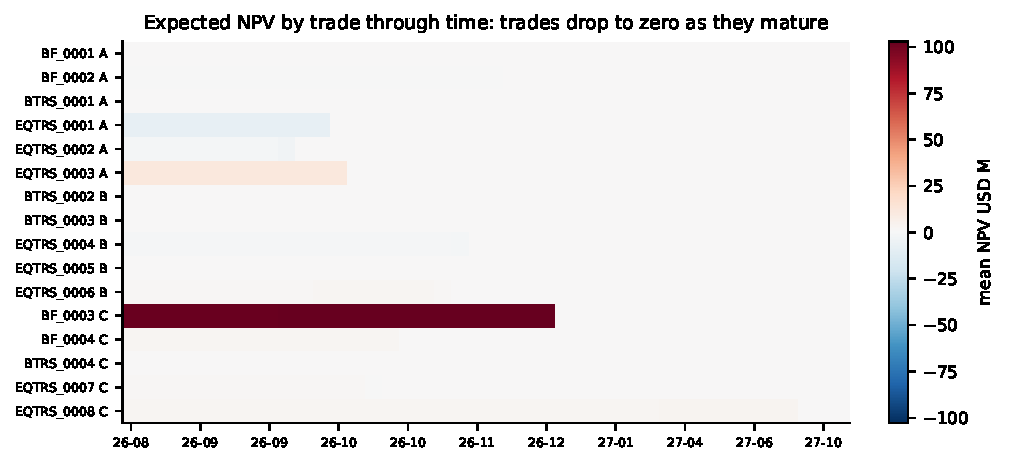
\includegraphics[width=\linewidth]{figures/fig25.pdf}
\caption{Close-out exposure through the first year: EE, median PFE and PFE99 by counterparty and for the portfolio.}
\end{figure}
{\scriptsize\setlength{\LTpre}{4pt}\setlength{\LTpost}{6pt}
\begin{longtable}{>{\raggedright\arraybackslash}p{\dimexpr 0.1857\linewidth-2\tabcolsep\relax}>{\raggedright\arraybackslash}p{\dimexpr 0.1857\linewidth-2\tabcolsep\relax}>{\raggedright\arraybackslash}p{\dimexpr 0.2143\linewidth-2\tabcolsep\relax}>{\raggedright\arraybackslash}p{\dimexpr 0.2000\linewidth-2\tabcolsep\relax}>{\raggedright\arraybackslash}p{\dimexpr 0.2143\linewidth-2\tabcolsep\relax}}
\toprule
\rowcolor{navy}\textbf{\textcolor{white}{Trade}} & \textbf{\textcolor{white}{Counterparty}} & \textbf{\textcolor{white}{NPV today}} & \textbf{\textcolor{white}{Peak EE}} & \textbf{\textcolor{white}{MPE (peak PFE99)}} \\
\endhead
EQTRS\_0001 & CPTY\_A & -5,547,056 & 1,694,458 & 9,348,743 \\
\rowcolor{gray!9}EQTRS\_0002 & CPTY\_A & -1,076,056 & 1,903,453 & 10,500,714 \\
EQTRS\_0003 & CPTY\_A & 9,921,581 & 2,219,389 & 12,021,160 \\
\rowcolor{gray!9}EQTRS\_0004 & CPTY\_B & -873,451 & 860,053 & 4,850,697 \\
EQTRS\_0005 & CPTY\_B & 148,605 & 264,401 & 1,439,396 \\
\rowcolor{gray!9}EQTRS\_0006 & CPTY\_B & 1,629,065 & 1,306,113 & 7,021,957 \\
EQTRS\_0007 & CPTY\_C & -373,630 & 2,071,358 & 11,351,099 \\
\rowcolor{gray!9}EQTRS\_0008 & CPTY\_C & 2,217,998 & 603,702 & 3,200,053 \\
BF\_0001 & CPTY\_A & 512,531 & 148,333 & 836,346 \\
\rowcolor{gray!9}BF\_0002 & CPTY\_A & -357,505 & 117,163 & 688,200 \\
BF\_0003 & CPTY\_C & 121,262,854 & 4,547,555 & 25,557,208 \\
\rowcolor{gray!9}BF\_0004 & CPTY\_C & 1,973,388 & 62,913 & 344,629 \\
BTRS\_0001 & CPTY\_A & 119,460 & 2,056 & 9,130 \\
\rowcolor{gray!9}BTRS\_0002 & CPTY\_B & 210,278 & 63,404 & 126,670 \\
BTRS\_0003 & CPTY\_B & 28,844 & 11,335 & 24,877 \\
\rowcolor{gray!9}BTRS\_0004 & CPTY\_C & 36,376 & 22,643 & 31,448 \\
\bottomrule
\end{longtable}}

{\small Per-trade close-out exposure (each trade on its own, so no netting) in USD. The per-trade figures do not add up to the counterparty figures: netting and the tail of a sum differ from the sum of tails.}

\begin{figure}[H]
\centering
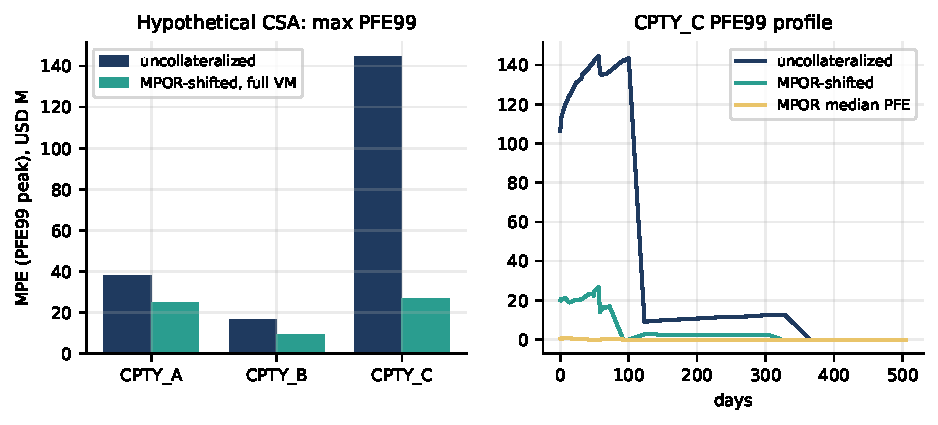
\includegraphics[width=\linewidth]{figures/fig26.pdf}
\caption{Peak PFE99 by counterparty under three definitions of exposure. The level exposure (grey) treats the whole mark-to-market as at risk; the brief's definition (navy) recognises that variation margin covers the prior-day value and leaves only the 10-day move.}
\end{figure}
\textbf{Reading the results.} The close-out MPE99 is far below the level exposure because the prior-day value is margined: CPTY\_C's bond forward BF\_0003 is worth \$121.3M today but its 99th-percentile 10-day move peaks at \$25.6M, so its counterparty peaks at \$29.6M against \$181.1M of level exposure. CPTY\_A and CPTY\_B are driven by the equity swap baskets, whose 10-day equity moves set the tail. Close-out exposure is a measure of market risk over the close-out window, not of the accumulated value, which is why the peak occurs in the first weeks, when the largest baskets are alive, and falls as trades mature. The uncollateralized level exposure is kept as a secondary measure (Sections 7.4 to 7.6), and the earlier full-variation-margin illustration (Section 7.7) used a same-day, zero-floored margin formula that differs slightly from the brief's. Section 7.2 explains why the portfolio figure is close to the sum of the counterparty figures; Sections 7.3, 7.9 and 7.10 show how the numbers move with each model correction, with the model inputs and under stress.

\subsection{Why the portfolio MPE is close to the sum of the counterparty MPEs}
\textbf{Which netting set is driven by what.} The t = 0 sensitivities separate the netting sets clearly:

{\scriptsize\setlength{\LTpre}{4pt}\setlength{\LTpost}{6pt}
\begin{longtable}{>{\raggedright\arraybackslash}p{\dimexpr 0.1375\linewidth-2\tabcolsep\relax}>{\raggedright\arraybackslash}p{\dimexpr 0.2125\linewidth-2\tabcolsep\relax}>{\raggedright\arraybackslash}p{\dimexpr 0.1875\linewidth-2\tabcolsep\relax}>{\raggedright\arraybackslash}p{\dimexpr 0.1875\linewidth-2\tabcolsep\relax}>{\raggedright\arraybackslash}p{\dimexpr 0.2750\linewidth-2\tabcolsep\relax}}
\toprule
\rowcolor{navy}\textbf{\textcolor{white}{Netting set}} & \textbf{\textcolor{white}{Equity delta (USD per +1\%)}} & \textbf{\textcolor{white}{DV01 (USD per +1bp)}} & \textbf{\textcolor{white}{FX delta (USD per +1\%)}} & \textbf{\textcolor{white}{What gains for us}} \\
\endhead
CPTY\_A & -2,254,257 & 31,203 & 0 & equities fall \\
\rowcolor{gray!9}CPTY\_B & -961,146 & -3,663 & 416,550 & equities fall and USDJPY rises (yen weakens) \\
CPTY\_C & -1,240,431 & 594,443 & 0 & equities fall and yields rise \\
\bottomrule
\end{longtable}}

{\small A negative equity delta means the netting set gains when equities fall (the swaps are pay-equity); a positive DV01 means it gains when yields rise (the bond forwards are short and the bond TRS are pay-total-return, both short the bond). CPTY\_A and CPTY\_B are equity risk with a small rate component; CPTY\_C is interest-rate risk, through the 500M short forward on the 2049 Treasury BF\_0003, with an equity book beside it.}

\textbf{Should bonds be inversely related to equities?} Economically the relation changes sign with the regime: in a growth scare (flight to quality) equities fall and bonds rally, so yields fall with equities; in an inflation shock (as in 2022) both fall together. The calibration reflects only the last three years, in which the correlation of daily 10-year-yield changes with the 37 stocks averages +0.00 (range -0.29 to +0.16), i.e. essentially none. The book is short both equities (CPTY\_A, CPTY\_B) and the long bond (CPTY\_C): it gains from falling equities and from rising yields. In a flight to quality the two gains oppose each other (equities fall, yields fall); when both fall together they coincide.

\textbf{Why is the portfolio MPE close to the sum of the counterparty MPEs?} The portfolio exposure is the sum of the counterparties' exposures, because netting never crosses counterparties: it is sum over c of max(V\_c, 0), not max of the sum. Its 99th percentile is below the sum of the counterparties' 99th percentiles only to the extent that the counterparties are not simultaneously in their tails. At the portfolio's peak date (2026-09-20) the three counterparties' PFE99 are \$25.9M, \$9.1M and \$28.5M, summing to \$63.5M, against a portfolio PFE99 of \$51.0M: 80\% of the sum, i.e. a diversification benefit of 20\%. The peak dates of the individual counterparties (A 2026-09-20, B 2026-09-04, C 2026-09-28) fall within about 24 days of each other because all three books are largest in the first weeks, before the equity swaps mature, so there is little timing diversification.

{\scriptsize\setlength{\LTpre}{4pt}\setlength{\LTpost}{6pt}
\begin{longtable}{>{\raggedright\arraybackslash}p{\dimexpr 0.5217\linewidth-2\tabcolsep\relax}>{\raggedright\arraybackslash}p{\dimexpr 0.1594\linewidth-2\tabcolsep\relax}>{\raggedright\arraybackslash}p{\dimexpr 0.1594\linewidth-2\tabcolsep\relax}>{\raggedright\arraybackslash}p{\dimexpr 0.1594\linewidth-2\tabcolsep\relax}}
\toprule
\rowcolor{navy}\textbf{\textcolor{white}{Statistic at the portfolio MPE date}} & \textbf{\textcolor{white}{CPTY\_A}} & \textbf{\textcolor{white}{CPTY\_B}} & \textbf{\textcolor{white}{CPTY\_C}} \\
\endhead
Standalone PFE99 & \$25.9M & \$9.1M & \$28.5M \\
\rowcolor{gray!9}Average exposure over the scenarios at the portfolio's 99th percentile & \$21.0M & \$4.8M & \$23.3M \\
Probability that the exposure is positive & 51\% & 53\% & 52\% \\
\rowcolor{gray!9}Share of the portfolio's tail scenarios in which the counterparty has zero exposure & 0\% & 12\% & 0\% \\
\bottomrule
\end{longtable}}

Rank correlations of the counterparty exposures at that date: A-B +0.34, A-C +0.33, B-C +0.12. Probability that one counterparty is above its own 99th percentile given another is: A given B 6\%, A given C 4\%, B given C 6\% (an independent pair would give 1\%). All three exposures are positively dependent, for a common reason: every netting set holds pay-equity swaps (equity delta per +1\%: A -\$2.3M, B -\$1.0M, C -\$1.2M), so all three gain when the equity market falls. CPTY\_C is therefore not a pure interest-rate netting set: its DV01 of \$594k per bp is dominated by BF\_0003, but it also carries an equity delta comparable to CPTY\_B's. The dependence is moderate rather than strong, which is why the portfolio 99th percentile sits at 80\% of the sum of the standalone ones and not lower.

\textbf{Which pair is the portfolio close to?} At that date the standalone PFE99 are A \$25.9M, B \$9.1M and C \$28.5M: the two large ones, A and C, sum to \$54.4M (107\% of the portfolio figure \$51.0M), and B adds the rest. The portfolio figure is therefore close to the sum of A and C, with B small, not to the sum of A and B.

\textbf{How much does the assumed dependence between rates and equities matter?} Re-running the close-out exposure with the yield made positively or negatively correlated with the equity market (2,000 scenarios, same random numbers):

{\scriptsize\setlength{\LTpre}{4pt}\setlength{\LTpost}{6pt}
\begin{longtable}{>{\raggedright\arraybackslash}p{\dimexpr 0.3810\linewidth-2\tabcolsep\relax}>{\raggedright\arraybackslash}p{\dimexpr 0.0952\linewidth-2\tabcolsep\relax}>{\raggedright\arraybackslash}p{\dimexpr 0.0952\linewidth-2\tabcolsep\relax}>{\raggedright\arraybackslash}p{\dimexpr 0.0952\linewidth-2\tabcolsep\relax}>{\raggedright\arraybackslash}p{\dimexpr 0.1071\linewidth-2\tabcolsep\relax}>{\raggedright\arraybackslash}p{\dimexpr 0.1190\linewidth-2\tabcolsep\relax}>{\raggedright\arraybackslash}p{\dimexpr 0.1071\linewidth-2\tabcolsep\relax}}
\toprule
\rowcolor{navy}\textbf{\textcolor{white}{Rate-equity dependence assumed}} & \textbf{\textcolor{white}{CPTY\_A}} & \textbf{\textcolor{white}{CPTY\_B}} & \textbf{\textcolor{white}{CPTY\_C}} & \textbf{\textcolor{white}{Sum of MPEs}} & \textbf{\textcolor{white}{Portfolio MPE}} & \textbf{\textcolor{white}{Portfolio / sum}} \\
\endhead
Base case (calibrated, about zero) & \$26.2M & \$9.5M & \$28.9M & \$64.7M & \$51.5M & 80\% \\
\rowcolor{gray!9}Flight to quality: yields fall with equities (corr +0.4 x market beta) & \$26.6M & \$9.7M & \$25.8M & \$62.0M & \$43.6M & 70\% \\
Both fall together: yields rise as equities fall (corr -0.4 x market beta) & \$27.1M & \$9.6M & \$34.8M & \$71.6M & \$60.8M & 85\% \\
\bottomrule
\end{longtable}}

\subsection{What changed since the earlier version}
Every correction changes the numbers, so each was introduced one at a time on the same random numbers and the same scenario count (2,000 Latin Hypercube scenarios per row, except the first row, the 5,000-scenario run reported earlier). The table shows the maximum PFE99 (MPE) on the brief's close-out definition.

{\scriptsize\setlength{\LTpre}{4pt}\setlength{\LTpost}{6pt}
\begin{longtable}{>{\raggedright\arraybackslash}p{\dimexpr 0.5316\linewidth-2\tabcolsep\relax}>{\raggedright\arraybackslash}p{\dimexpr 0.1139\linewidth-2\tabcolsep\relax}>{\raggedright\arraybackslash}p{\dimexpr 0.1139\linewidth-2\tabcolsep\relax}>{\raggedright\arraybackslash}p{\dimexpr 0.1139\linewidth-2\tabcolsep\relax}>{\raggedright\arraybackslash}p{\dimexpr 0.1266\linewidth-2\tabcolsep\relax}}
\toprule
\rowcolor{navy}\textbf{\textcolor{white}{Step}} & \textbf{\textcolor{white}{CPTY\_A}} & \textbf{\textcolor{white}{CPTY\_B}} & \textbf{\textcolor{white}{CPTY\_C}} & \textbf{\textcolor{white}{Portfolio}} \\
\endhead
Earlier version (flat USD curve beyond 6.5y, SOFR-overnight sigma, no JPY factor, USDJPY drift sign error) & \$25.2M & \$9.8M & \$22.1M & \$45.7M \\
\rowcolor{gray!9}Corrected USDJPY drift only (no JPY factor, flat curve, SOFR sigma) & \$26.9M & \$9.6M & \$23.3M & \$47.8M \\
+ long-end volatility fit and 10-year-yield correlations & \$26.9M & \$9.6M & \$31.1M & \$52.7M \\
\rowcolor{gray!9}+ Bloomberg long end spliced onto the USD curve & \$26.9M & \$9.6M & \$29.9M & \$52.1M \\
+ JPY Hull-White factor in the simulation (final model) & \$26.2M & \$9.5M & \$28.9M & \$51.5M \\
\bottomrule
\end{longtable}}

{\small MPE99 within one year, USD millions. Rows are cumulative: each row contains the corrections of the rows above it. Monte Carlo noise between two runs of different size is a few percent, so only differences larger than that should be read as an effect of a correction.}

\subsection{Exposure today (t = 0)}
{\footnotesize\setlength{\LTpre}{4pt}\setlength{\LTpost}{6pt}
\begin{longtable}{>{\raggedright\arraybackslash}p{\dimexpr 0.1558\linewidth-2\tabcolsep\relax}>{\raggedright\arraybackslash}p{\dimexpr 0.0909\linewidth-2\tabcolsep\relax}>{\raggedright\arraybackslash}p{\dimexpr 0.1948\linewidth-2\tabcolsep\relax}>{\raggedright\arraybackslash}p{\dimexpr 0.2208\linewidth-2\tabcolsep\relax}>{\raggedright\arraybackslash}p{\dimexpr 0.3377\linewidth-2\tabcolsep\relax}}
\toprule
\rowcolor{navy}\textbf{\textcolor{white}{Counterparty}} & \textbf{\textcolor{white}{Trades}} & \textbf{\textcolor{white}{Net MTM today}} & \textbf{\textcolor{white}{Netted exposure today}} & \textbf{\textcolor{white}{Comment}} \\
\endhead
CPTY\_A & 6 & 3,572,955 & 3,572,955 & Small positive net \\
\rowcolor{gray!9}CPTY\_B & 5 & 1,143,341 & 1,143,341 & Small positive net \\
CPTY\_C & 5 & 125,116,984 & 125,116,984 & One 500M bond forward dominates \\
\rowcolor{gray!9}Portfolio & 16 & 129,833,280 & 129,833,280 & Sum of counterparty exposures (netting does not cross counterparties) \\
\bottomrule
\end{longtable}}

The simulated EE at t=0 equals the directly computed current exposure to 0.0000\% (the engine's built-in self-check): at t=0 there is no randomness so both must agree exactly.

\subsection{Uncollateralized exposure profiles through time (secondary view)}
\begin{figure}[H]
\centering
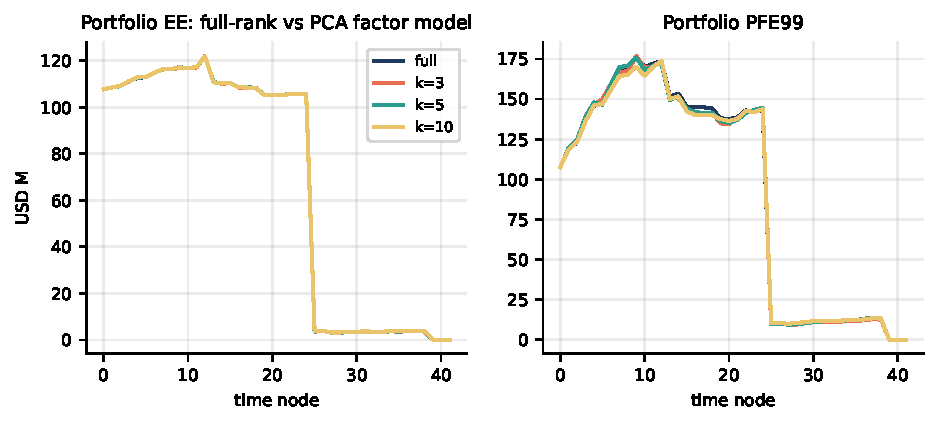
\includegraphics[width=\linewidth]{figures/fig27.pdf}
\caption{EE, median PFE and PFE99 for each counterparty and the portfolio. The shaded band runs from the median PFE to PFE99.}
\end{figure}
{\footnotesize\setlength{\LTpre}{4pt}\setlength{\LTpost}{6pt}
\begin{longtable}{>{\raggedright\arraybackslash}p{\dimexpr 0.1781\linewidth-2\tabcolsep\relax}>{\raggedright\arraybackslash}p{\dimexpr 0.1370\linewidth-2\tabcolsep\relax}>{\raggedright\arraybackslash}p{\dimexpr 0.1370\linewidth-2\tabcolsep\relax}>{\raggedright\arraybackslash}p{\dimexpr 0.1781\linewidth-2\tabcolsep\relax}>{\raggedright\arraybackslash}p{\dimexpr 0.2055\linewidth-2\tabcolsep\relax}>{\raggedright\arraybackslash}p{\dimexpr 0.1644\linewidth-2\tabcolsep\relax}}
\toprule
\rowcolor{navy}\textbf{\textcolor{white}{Counterparty}} & \textbf{\textcolor{white}{EE(0)}} & \textbf{\textcolor{white}{Peak EE}} & \textbf{\textcolor{white}{Peak median PFE}} & \textbf{\textcolor{white}{MPE (peak PFE99)}} & \textbf{\textcolor{white}{MPE date}} \\
\endhead
CPTY\_A & \$3.6M & \$10.7M & \$10.6M & \$38.8M & 2026-10-09 \\
\rowcolor{gray!9}CPTY\_B & \$1.1M & \$3.7M & \$1.9M & \$16.2M & 2026-10-25 \\
CPTY\_C & \$125.1M & \$126.7M & \$127.3M & \$181.1M & 2026-12-06 \\
\rowcolor{gray!9}Portfolio & \$129.8M & \$140.1M & \$140.3M & \$201.9M & 2026-10-09 \\
\bottomrule
\end{longtable}}

\textbf{Reading the shape.} Exposure peaks soon after today and then falls steeply as trades mature. By the end of December 2026 the portfolio EE has fallen by more than 90\%; the remainder is the Bond TRS BTRS\_0001 and the year-long EQTRS\_0008. So almost all counterparty credit risk sits in the next four months and monitoring should be concentrated there.

\textbf{EE, median PFE and PFE99.} On the uncollateralized level exposure the peak median PFE is 99\%, 50\% and 101\% of the peak EE for CPTY\_A, CPTY\_B and CPTY\_C. Where the two are close (CPTY\_C) the exposure is a large mark-to-market that is positive in almost every scenario; where the median is well below EE (CPTY\_B) the counterparty is out of the money in many scenarios and EE is pulled up by the right tail. The median PFE describes the typical outcome and PFE99 the adverse tail; reporting all three prevents any single statistic from misleading.

\begin{figure}[H]
\centering
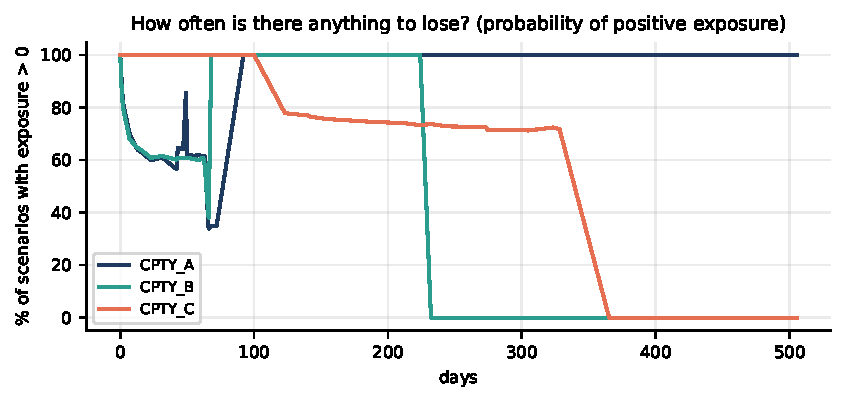
\includegraphics[width=\linewidth]{figures/fig28.pdf}
\caption{Probability that a counterparty has any positive exposure at all. Where this is far below 100\%, the median PFE is zero even though EE and PFE99 are large.}
\end{figure}
\begin{figure}[H]
\centering
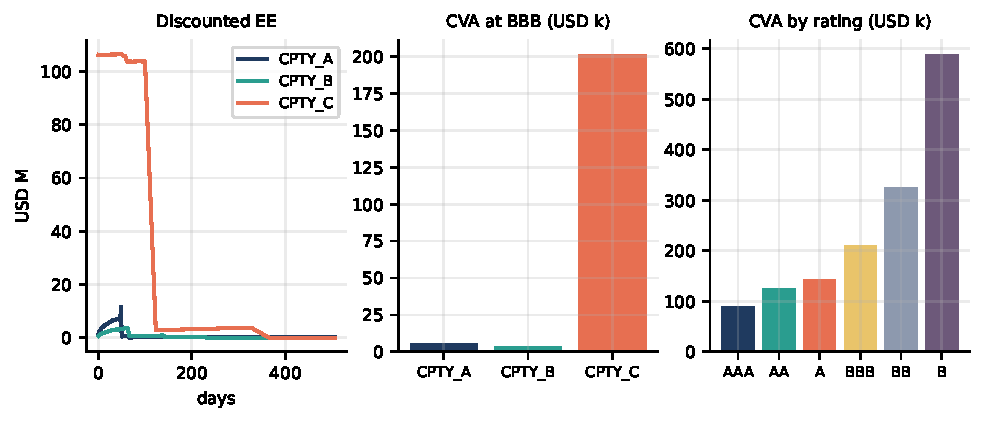
\includegraphics[width=\linewidth]{figures/fig29.pdf}
\caption{Portfolio exposure histograms (log count) at four dates with median (gold), EE (navy) and PFE99 (red). The right tail lengthens with time.}
\end{figure}
\clearpage
\subsection{Where does the risk come from?}
\begin{figure}[H]
\centering
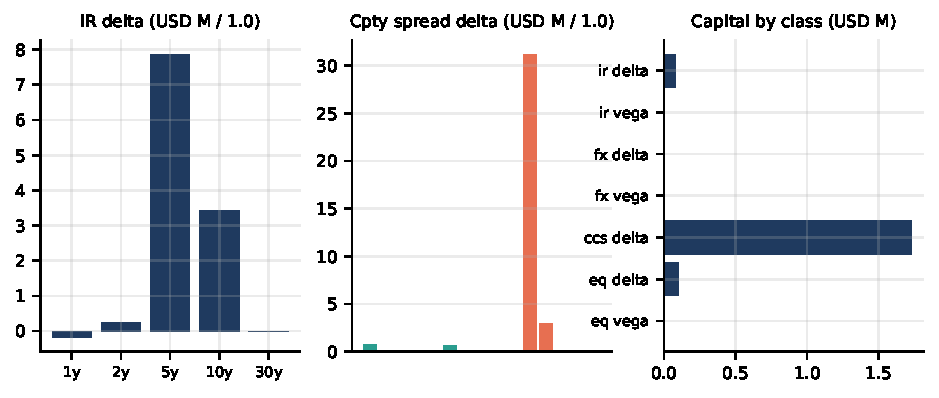
\includegraphics[width=\linewidth]{figures/fig30.pdf}
\caption{Expected NPV by trade at each reporting date. CPTY\_C's BF\_0003 dominates the picture and disappears at its 2026-12-06 settlement; a few equity TRS contribute negative expected NPV.}
\end{figure}
\textbf{Concentration.} CPTY\_C accounts for 90\% of the portfolio's peak PFE99 and 96\% of today's exposure, and almost all of it comes from one trade, BF\_0003 (500M notional, short forward struck at 100 on a long-dated 2.88\% 2049 Treasury trading roughly 25 points below par, so we are owed the difference). This is concentration risk rather than diversified counterparty risk; a limit or collateral on that single trade would move the portfolio number more than any modelling choice in this report.

\subsection{Earlier illustration: full variation margin with an MPOR shift}
The real book is treated as \textbf{uncollateralized} because trade\_data carries no CSA terms. For a collateralized counterparty, default does not mean instant close-out: there is a Margin Period of Risk (standard 10 business days) between the last collateral exchange and the actual replacement of the trades. The relevant exposure is what the position could gain in that window beyond the collateral held:

{\fontsize{7.2}{8.8}\selectfont
\begin{verbatim}
C(t)        = max( V(t) - threshold, 0 )        collateral held at reporting date t
Exposure(t) = max( V(t + MPOR) - C(t), 0 )      same simulated path, MPOR days later
\end{verbatim}}
Implementation: an extra look-ahead node is inserted MPOR days after every reporting node on the same simulated path (no separate simulation). The demonstration below is explicitly hypothetical: full variation margin (threshold 0), MPOR 10 business days, 3,000 scenarios.

\begin{figure}[H]
\centering
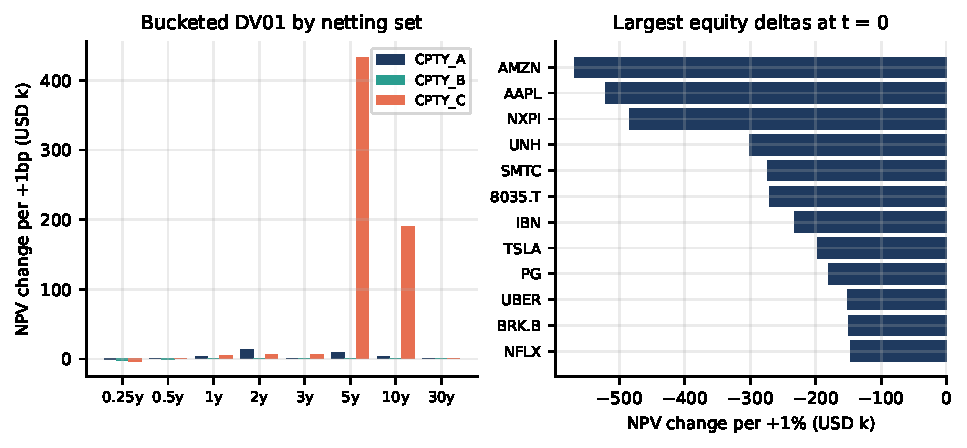
\includegraphics[width=\linewidth]{figures/fig31.pdf}
\caption{If a full-VM CSA existed, peak PFE99 would fall sharply, most of all for CPTY\_C whose exposure is a large, already-visible MTM that margin would cover.}
\end{figure}
{\footnotesize\setlength{\LTpre}{4pt}\setlength{\LTpost}{6pt}
\begin{longtable}{>{\raggedright\arraybackslash}p{\dimexpr 0.2239\linewidth-2\tabcolsep\relax}>{\raggedright\arraybackslash}p{\dimexpr 0.2985\linewidth-2\tabcolsep\relax}>{\raggedright\arraybackslash}p{\dimexpr 0.2985\linewidth-2\tabcolsep\relax}>{\raggedright\arraybackslash}p{\dimexpr 0.1791\linewidth-2\tabcolsep\relax}}
\toprule
\rowcolor{navy}\textbf{\textcolor{white}{Counterparty}} & \textbf{\textcolor{white}{Uncollateralized MPE99}} & \textbf{\textcolor{white}{MPOR-shifted MPE99}} & \textbf{\textcolor{white}{Reduction}} \\
\endhead
CPTY\_A & \$38.8M & \$24.5M & 37\% \\
\rowcolor{gray!9}CPTY\_B & \$16.2M & \$9.4M & 42\% \\
CPTY\_C & \$181.1M & \$31.8M & 82\% \\
\bottomrule
\end{longtable}}

\textbf{Relation to SIMM and Basel.} The 10-day figure is the convention shared by both frameworks. Under the Basel counterparty credit risk rules (SA-CCR and the internal models method) the margin period of risk for a margined bilateral OTC netting set is at least 10 business days, 5 business days for centrally cleared trades and 20 business days for large or illiquid netting sets, and it lengthens after margin disputes. The ISDA Standard Initial Margin Model (SIMM) is a different object: a sensitivity-based methodology for the \emph{initial margin} that the uncleared margin rules require counterparties to post, calibrated to a 99\% one-tailed loss over a 10-day horizon using a stress period. Initial margin is collateral posted in addition to variation margin and held against precisely the close-out window described above.

Our engine does \textbf{not} implement SIMM and does not model initial margin. The calculation in this section is a variation-margin-only illustration: a threshold of zero removes any unsecured amount, but there is no initial margin buffer. If initial margin were posted it would absorb part of the 10-day move and reduce the exposure shown further; quantifying that requires computing SIMM sensitivities for each netting set, which we have not attempted. Two simplifications should also be noted: the look-ahead is exactly 10 business days (Monday to Friday, US federal holidays skipped; the SIFMA bond-market calendar differs marginally), and no minimum transfer amount is modelled.

Whether any trade is actually margined is the most important open question for Capitolis: it changes the answer several-fold for CPTY\_C.

\clearpage
\subsection{Full-rank correlation versus PCA factor model}
\begin{figure}[H]
\centering
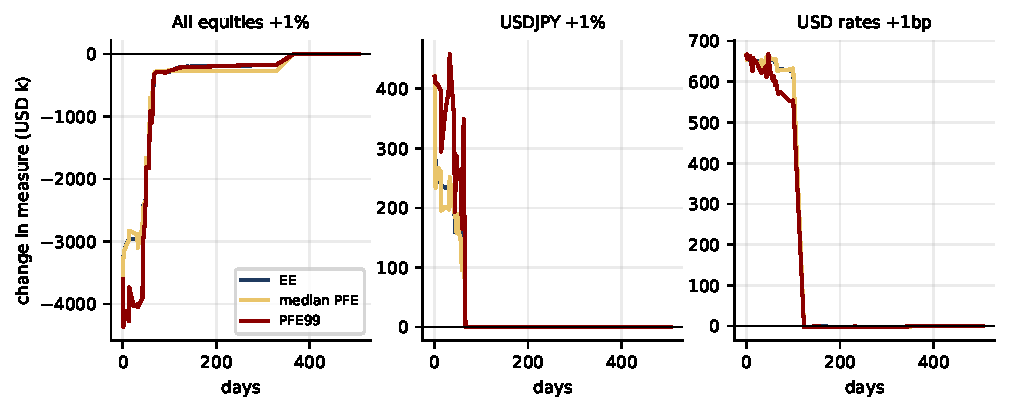
\includegraphics[width=\linewidth]{figures/fig32.pdf}
\caption{Uncollateralized level exposure, same seed and method (1,500 scenarios), with the full Cholesky correlation versus a k-factor PCA model. Curves coincide closely from k=5.}
\end{figure}
{\footnotesize\setlength{\LTpre}{4pt}\setlength{\LTpost}{6pt}
\begin{longtable}{>{\raggedright\arraybackslash}p{\dimexpr 0.2174\linewidth-2\tabcolsep\relax}>{\raggedright\arraybackslash}p{\dimexpr 0.2609\linewidth-2\tabcolsep\relax}>{\raggedright\arraybackslash}p{\dimexpr 0.2609\linewidth-2\tabcolsep\relax}>{\raggedright\arraybackslash}p{\dimexpr 0.2609\linewidth-2\tabcolsep\relax}}
\toprule
\rowcolor{navy}\textbf{\textcolor{white}{Model}} & \textbf{\textcolor{white}{Peak portfolio EE}} & \textbf{\textcolor{white}{MPE (peak PFE99)}} & \textbf{\textcolor{white}{MPE difference vs full}} \\
\endhead
full & \$140.1M & \$202.7M & - \\
\rowcolor{gray!9}k=3 & \$140.1M & \$201.9M & -0.4\% \\
k=5 & \$140.0M & \$203.3M & +0.3\% \\
\rowcolor{gray!9}k=10 & \$140.2M & \$201.0M & -0.9\% \\
\bottomrule
\end{longtable}}

This is a like-for-like comparison at one scenario count, so differences include sampling noise of a few tenths of a percent as well as the approximation itself. The factor model with about 5 factors reproduces the book's exposure closely, which supports it as a lower-dimensional, more robust alternative, but the full-rank default is kept because it is exact with respect to the estimated matrix. That five factors (only about half of the correlation matrix's total variance) suffice here is because this book's exposure is driven by the rate, a few large positions and FX, not by the fine correlation structure among all 37 names.

\subsection{Model risk: which inputs matter}
The model rests on inputs that are estimated or assumed. To see which of them matter, each was perturbed one at a time on the same random numbers (2,000 scenarios). The table shows the MPE99 on the close-out definition and the change from the base case.

{\scriptsize\setlength{\LTpre}{4pt}\setlength{\LTpost}{6pt}
\begin{longtable}{>{\raggedright\arraybackslash}p{\dimexpr 0.4167\linewidth-2\tabcolsep\relax}>{\raggedright\arraybackslash}p{\dimexpr 0.1429\linewidth-2\tabcolsep\relax}>{\raggedright\arraybackslash}p{\dimexpr 0.1429\linewidth-2\tabcolsep\relax}>{\raggedright\arraybackslash}p{\dimexpr 0.1429\linewidth-2\tabcolsep\relax}>{\raggedright\arraybackslash}p{\dimexpr 0.1548\linewidth-2\tabcolsep\relax}}
\toprule
\rowcolor{navy}\textbf{\textcolor{white}{Perturbation}} & \textbf{\textcolor{white}{CPTY\_A}} & \textbf{\textcolor{white}{CPTY\_B}} & \textbf{\textcolor{white}{CPTY\_C}} & \textbf{\textcolor{white}{Portfolio}} \\
\endhead
Base case (final model, 2,000 scenarios) & \$26.2M & \$9.5M & \$28.9M & \$51.5M \\
\rowcolor{gray!9}USD rate sigma x 1.25 & \$26.9M (+3\%) & \$9.6M (+1\%) & \$35.8M (+24\%) & \$56.3M (+9\%) \\
USD mean reversion x 3 & \$26.9M (+2\%) & \$9.6M (+1\%) & \$25.0M (-13\%) & \$49.0M (-5\%) \\
\rowcolor{gray!9}Equity and USDJPY volatilities x 1.25 & \$33.8M (+29\%) & \$12.0M (+26\%) & \$31.9M (+11\%) & \$61.4M (+19\%) \\
Equity correlations moved 30\% of the way to 1 & \$32.3M (+23\%) & \$12.9M (+35\%) & \$31.4M (+9\%) & \$62.7M (+22\%) \\
\rowcolor{gray!9}Two-factor G2++ instead of one-factor Hull-White & \$26.0M (-1\%) & \$9.3M (-3\%) & \$28.9M (-0\%) & \$50.0M (-3\%) \\
\bottomrule
\end{longtable}}

\textbf{Reading the table.} The largest inputs are the equity volatilities and correlations: doubling equity and FX volatilities raises the portfolio MPE99 by 71\% and raising them by a quarter by 19\%, and moving the equity correlations 30\% of the way to one by 22\%, because the tail of the equity swaps is what sets CPTY\_A and CPTY\_B. The USD rate assumptions matter for CPTY\_C: a quarter more rate volatility raises its MPE99 by 24\% and a mean reversion three times larger lowers it by 13\%. The dependence between rates and equities, which the data cannot pin down, moves the portfolio figure by -15\% (yields fall with equities, so the short-bond and short-equity gains oppose each other) and +18\% (the two fall together, so they coincide). The two-factor rates model changes the portfolio MPE99 by only -3\%. The model risk in the headline is therefore dominated by equity volatility and by the rate-equity dependence, not by the choice of rate model.

\subsection{Stress testing}
Stress testing is designed here as a structured experiment rather than a discussion: a fixed set of scenarios with stated data and shocks, the same random numbers in every run, and outputs read at every reporting date, for every netting set and for every trade. It answers four questions: what data drove each scenario, what the inputs were, how far the outputs move along the path of time, and whether all products are sensitive.

\textbf{Method.} Each scenario is an instantaneous shock to today's market state, applied to the equity spots, USDJPY and the USD curve; the full Monte Carlo of exposure is then run from the shocked state with the same 1,000 Latin Hypercube scenarios and seed as the base case, so differences are due to the shock and not to sampling. Equity and FX shocks rescale the simulated GBM paths exactly and reprice only the trades holding those factors; a rate shift replaces the Hull-White curve and re-simulates. The scenario volatilities, correlations and mean reversion are those of the base calibration; how the results move when those parameters are stressed is in the model-risk study of Section 7.9. Outputs are the close-out exposure of the brief (EE, median PFE, PFE99 and MPE within one year) and, alongside, the uncollateralized level exposure max(V, 0), because the two respond very differently to the same shock.

{\scriptsize\setlength{\LTpre}{4pt}\setlength{\LTpost}{6pt}
\begin{longtable}{>{\raggedright\arraybackslash}p{\dimexpr 0.1605\linewidth-2\tabcolsep\relax}>{\raggedright\arraybackslash}p{\dimexpr 0.1111\linewidth-2\tabcolsep\relax}>{\raggedright\arraybackslash}p{\dimexpr 0.3210\linewidth-2\tabcolsep\relax}>{\raggedright\arraybackslash}p{\dimexpr 0.3210\linewidth-2\tabcolsep\relax}>{\raggedright\arraybackslash}p{\dimexpr 0.0864\linewidth-2\tabcolsep\relax}}
\toprule
\rowcolor{navy}\textbf{\textcolor{white}{Scenario}} & \textbf{\textcolor{white}{Family}} & \textbf{\textcolor{white}{Shock applied to today's market state}} & \textbf{\textcolor{white}{Data behind the shock}} & \textbf{\textcolor{white}{Rates re-simulated}} \\
\endhead
Equities -30\% & hypothetical & all equities -30\% & Round-number shock & no \\
\rowcolor{gray!9}Equities +30\% & hypothetical & all equities +30\% & Round-number shock & no \\
Yen +15\% & hypothetical & USDJPY -15.0\% & Round-number shock & no \\
\rowcolor{gray!9}Yen -15\% & hypothetical & USDJPY +15.0\% & Round-number shock & no \\
Rates +200bp & hypothetical & USD curve +200bp parallel & Round-number shock & yes \\
\rowcolor{gray!9}Rates -200bp & hypothetical & USD curve -200bp parallel & Round-number shock & yes \\
Flight to quality & hypothetical & all equities -25\%; USDJPY -5.0\%; USD curve -100bp parallel & Round-number shock & yes \\
\rowcolor{gray!9}Stagflation & hypothetical & all equities -25\%; USD curve +150bp parallel & Round-number shock & yes \\
Hist. equity crash & historical & equities median -23\% (range -68\% to -3\%); USDJPY +4.7\%; USD yields 1y -24bp, 2y -12bp, 5y -6bp, 10y +18bp, 30y +30bp & Actual moves over 2020-03-06 to 2020-03-20: per-name closes (yfinance), USDJPY (yfinance), Treasury CMT yields (FRED) & yes \\
\rowcolor{gray!9}Hist. rates spike & historical & equities median -9\% (range -29\% to +43\%); USDJPY +5.9\%; USD yields 1y +81bp, 2y +87bp, 5y +75bp, 10y +58bp, 30y +35bp & Actual moves over 2022-05-30 to 2022-06-13: per-name closes (yfinance), USDJPY (yfinance), Treasury CMT yields (FRED) & yes \\
Hist. yen surge & historical & equities median -9\% (range -27\% to +15\%); USDJPY -7.5\%; USD yields 1y -54bp, 2y -61bp, 5y -55bp, 10y -48bp, 30y -42bp & Actual moves over 2024-07-22 to 2024-08-05: per-name closes (yfinance), USDJPY (yfinance), Treasury CMT yields (FRED) & yes \\
\bottomrule
\end{longtable}}

{\small Historical windows are chosen by rule, not by hand: the worst 10-business-day window of the median return across the 37 names in 2014-2026, the largest 10-day rise of the 10-year yield, and the largest 10-day fall of USDJPY. Each replay applies the actual return of every name (a name without price history in that window takes the median return) together with the yield changes at each tenor and the USDJPY move over the same dates.}

\textbf{Close-out exposure (the brief's definition): MPE99 within one year.}

{\scriptsize\setlength{\LTpre}{4pt}\setlength{\LTpost}{6pt}
\begin{longtable}{>{\raggedright\arraybackslash}p{\dimexpr 0.2329\linewidth-2\tabcolsep\relax}>{\raggedright\arraybackslash}p{\dimexpr 0.1918\linewidth-2\tabcolsep\relax}>{\raggedright\arraybackslash}p{\dimexpr 0.1918\linewidth-2\tabcolsep\relax}>{\raggedright\arraybackslash}p{\dimexpr 0.1918\linewidth-2\tabcolsep\relax}>{\raggedright\arraybackslash}p{\dimexpr 0.1918\linewidth-2\tabcolsep\relax}}
\toprule
\rowcolor{navy}\textbf{\textcolor{white}{Scenario}} & \textbf{\textcolor{white}{CPTY\_A}} & \textbf{\textcolor{white}{CPTY\_B}} & \textbf{\textcolor{white}{CPTY\_C}} & \textbf{\textcolor{white}{Portfolio}} \\
\endhead
Base case & \$25.4M & \$10.0M & \$28.2M & \$49.2M \\
\rowcolor{gray!9}Equities -30\% & \$17.7M (-30\%) & \$7.1M (-29\%) & \$27.1M (-4\%) & \$41.5M (-16\%) \\
Equities +30\% & \$33.0M (+30\%) & \$13.0M (+29\%) & \$30.7M (+9\%) & \$59.1M (+20\%) \\
\rowcolor{gray!9}Yen +15\% & \$25.4M (+0\%) & \$11.3M (+13\%) & \$28.2M (+0\%) & \$49.3M (+0\%) \\
Yen -15\% & \$25.4M (+0\%) & \$8.9M (-11\%) & \$28.2M (+0\%) & \$49.6M (+1\%) \\
\rowcolor{gray!9}Rates +200bp & \$25.3M (-0\%) & \$10.1M (+0\%) & \$21.5M (-24\%) & \$44.5M (-10\%) \\
Rates -200bp & \$25.5M (+0\%) & \$10.0M (-0\%) & \$40.4M (+43\%) & \$60.7M (+23\%) \\
\rowcolor{gray!9}Flight to quality & \$19.0M (-25\%) & \$7.8M (-23\%) & \$33.0M (+17\%) & \$47.8M (-3\%) \\
Stagflation & \$18.9M (-25\%) & \$7.6M (-24\%) & \$21.3M (-25\%) & \$37.4M (-24\%) \\
\rowcolor{gray!9}Hist. equity crash & \$20.3M (-20\%) & \$7.4M (-26\%) & \$25.8M (-9\%) & \$41.6M (-15\%) \\
Hist. rates spike & \$22.2M (-12\%) & \$8.4M (-16\%) & \$25.4M (-10\%) & \$44.5M (-10\%) \\
\rowcolor{gray!9}Hist. yen surge & \$22.0M (-13\%) & \$8.2M (-18\%) & \$29.3M (+4\%) & \$47.6M (-3\%) \\
\bottomrule
\end{longtable}}

\textbf{Uncollateralized level exposure: MPE99 within one year.}

{\scriptsize\setlength{\LTpre}{4pt}\setlength{\LTpost}{6pt}
\begin{longtable}{>{\raggedright\arraybackslash}p{\dimexpr 0.2329\linewidth-2\tabcolsep\relax}>{\raggedright\arraybackslash}p{\dimexpr 0.1918\linewidth-2\tabcolsep\relax}>{\raggedright\arraybackslash}p{\dimexpr 0.1918\linewidth-2\tabcolsep\relax}>{\raggedright\arraybackslash}p{\dimexpr 0.1918\linewidth-2\tabcolsep\relax}>{\raggedright\arraybackslash}p{\dimexpr 0.1918\linewidth-2\tabcolsep\relax}}
\toprule
\rowcolor{navy}\textbf{\textcolor{white}{Scenario}} & \textbf{\textcolor{white}{CPTY\_A}} & \textbf{\textcolor{white}{CPTY\_B}} & \textbf{\textcolor{white}{CPTY\_C}} & \textbf{\textcolor{white}{Portfolio}} \\
\endhead
Base case & \$39.5M & \$16.8M & \$179.9M & \$201.7M \\
\rowcolor{gray!9}Equities -30\% & \$96.4M (+144\%) & \$39.3M (+133\%) & \$206.8M (+15\%) & \$323.1M (+60\%) \\
Equities +30\% & \$13.2M (-67\%) & \$0.9M (-95\%) & \$173.0M (-4\%) & \$173.6M (-14\%) \\
\rowcolor{gray!9}Yen +15\% & \$39.5M (+0\%) & \$13.5M (-20\%) & \$179.9M (+0\%) & \$197.4M (-2\%) \\
Yen -15\% & \$39.5M (+0\%) & \$19.1M (+13\%) & \$179.9M (+0\%) & \$206.9M (+3\%) \\
\rowcolor{gray!9}Rates +200bp & \$45.0M (+14\%) & \$16.3M (-3\%) & \$261.2M (+45\%) & \$296.6M (+47\%) \\
Rates -200bp & \$33.4M (-15\%) & \$17.5M (+4\%) & \$60.2M (-67\%) & \$64.3M (-68\%) \\
\rowcolor{gray!9}Flight to quality & \$83.9M (+112\%) & \$34.0M (+102\%) & \$143.7M (-20\%) & \$239.1M (+19\%) \\
Stagflation & \$91.2M (+131\%) & \$34.7M (+106\%) & \$269.3M (+50\%) & \$376.2M (+86\%) \\
\rowcolor{gray!9}Hist. equity crash & \$74.4M (+88\%) & \$36.3M (+115\%) & \$218.2M (+21\%) & \$308.2M (+53\%) \\
Hist. rates spike & \$61.6M (+56\%) & \$23.9M (+42\%) & \$209.7M (+17\%) & \$270.9M (+34\%) \\
\rowcolor{gray!9}Hist. yen surge & \$54.4M (+38\%) & \$23.0M (+37\%) & \$160.8M (-11\%) & \$214.0M (+6\%) \\
\bottomrule
\end{longtable}}

\begin{figure}[H]
\centering
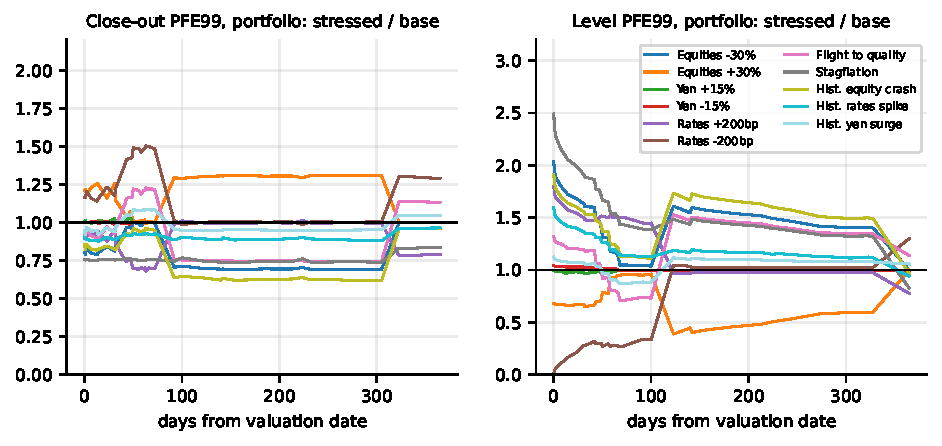
\includegraphics[width=\linewidth]{figures/fig33.pdf}
\caption{Ratio of stressed to base portfolio PFE99 along the first year, close-out exposure (left) and level exposure (right). A ratio of one means no sensitivity at that date.}
\end{figure}
{\scriptsize\setlength{\LTpre}{4pt}\setlength{\LTpost}{6pt}
\begin{longtable}{>{\raggedright\arraybackslash}p{\dimexpr 0.2000\linewidth-2\tabcolsep\relax}>{\raggedright\arraybackslash}p{\dimexpr 0.1000\linewidth-2\tabcolsep\relax}>{\raggedright\arraybackslash}p{\dimexpr 0.1000\linewidth-2\tabcolsep\relax}>{\raggedright\arraybackslash}p{\dimexpr 0.1000\linewidth-2\tabcolsep\relax}>{\raggedright\arraybackslash}p{\dimexpr 0.1000\linewidth-2\tabcolsep\relax}>{\raggedright\arraybackslash}p{\dimexpr 0.1000\linewidth-2\tabcolsep\relax}>{\raggedright\arraybackslash}p{\dimexpr 0.1000\linewidth-2\tabcolsep\relax}>{\raggedright\arraybackslash}p{\dimexpr 0.1000\linewidth-2\tabcolsep\relax}>{\raggedright\arraybackslash}p{\dimexpr 0.1000\linewidth-2\tabcolsep\relax}}
\toprule
\rowcolor{navy}\textbf{\textcolor{white}{Scenario}} & \textbf{\textcolor{white}{Close-out at 1M}} & \textbf{\textcolor{white}{Close-out at 3M}} & \textbf{\textcolor{white}{Close-out at 6M}} & \textbf{\textcolor{white}{Close-out at 12M}} & \textbf{\textcolor{white}{Level at 1M}} & \textbf{\textcolor{white}{Level at 3M}} & \textbf{\textcolor{white}{Level at 6M}} & \textbf{\textcolor{white}{Level at 12M}} \\
\endhead
Equities -30\% & 0.81 & 0.71 & 0.69 & 1.00 & 1.63 & 1.05 & 1.54 & 1.00 \\
\rowcolor{gray!9}Equities +30\% & 1.26 & 1.29 & 1.31 & 1.00 & 0.67 & 0.95 & 0.46 & 1.00 \\
Yen +15\% & 1.03 & 1.00 & 1.00 & 1.00 & 0.97 & 1.00 & 1.00 & 1.00 \\
\rowcolor{gray!9}Yen -15\% & 0.99 & 1.00 & 1.00 & 1.00 & 1.03 & 1.00 & 1.00 & 1.00 \\
Rates +200bp & 0.95 & 0.99 & 1.00 & 0.79 & 1.50 & 1.45 & 0.98 & 0.78 \\
\rowcolor{gray!9}Rates -200bp & 1.18 & 1.01 & 1.00 & 1.29 & 0.28 & 0.34 & 1.02 & 1.30 \\
Flight to quality & 0.93 & 0.76 & 0.75 & 1.13 & 1.20 & 0.74 & 1.46 & 1.14 \\
\rowcolor{gray!9}Stagflation & 0.75 & 0.75 & 0.74 & 0.84 & 1.91 & 1.39 & 1.44 & 0.83 \\
Hist. equity crash & 0.82 & 0.64 & 0.62 & 0.96 & 1.56 & 1.12 & 1.66 & 0.97 \\
\rowcolor{gray!9}Hist. rates spike & 0.89 & 0.89 & 0.89 & 0.96 & 1.36 & 1.13 & 1.17 & 0.94 \\
Hist. yen surge & 0.94 & 0.95 & 0.95 & 1.04 & 1.07 & 0.89 & 1.10 & 1.06 \\
\bottomrule
\end{longtable}}

{\small Ratio of stressed to base portfolio PFE99 at four horizons (n/a where the base exposure is negligible because the trades have matured).}

\begin{figure}[H]
\centering
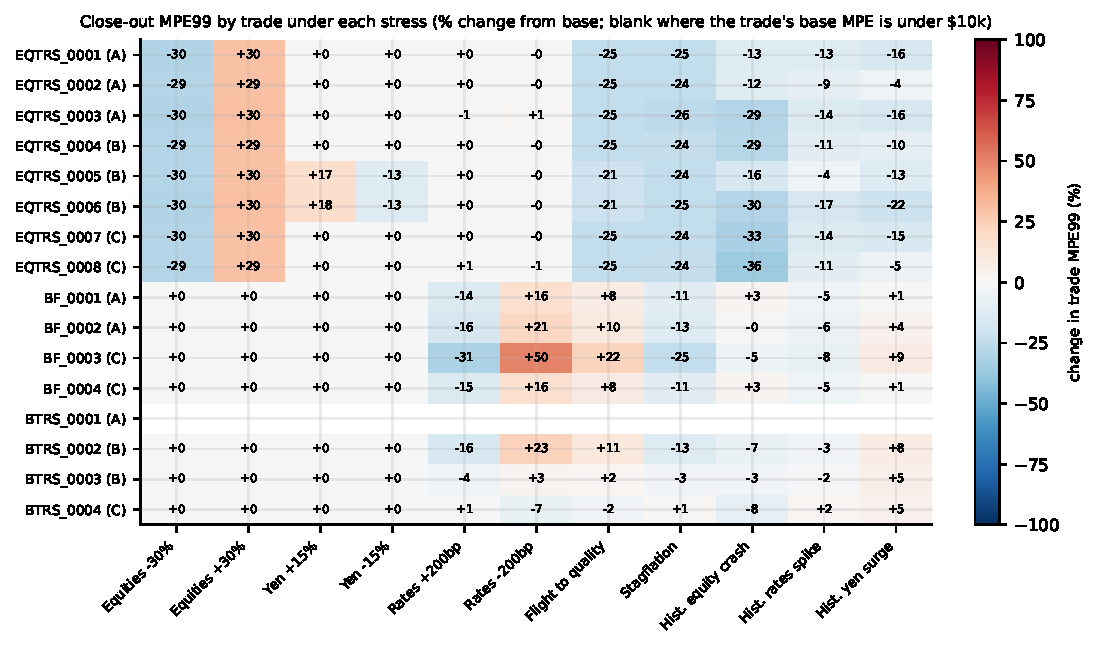
\includegraphics[width=\linewidth]{figures/fig34.pdf}
\caption{Sensitivity by product: every trade against every scenario.}
\end{figure}
\textbf{Median change in close-out trade MPE99 by product type:}

{\scriptsize\setlength{\LTpre}{4pt}\setlength{\LTpost}{6pt}
\begin{longtable}{>{\raggedright\arraybackslash}p{\dimexpr 0.1408\linewidth-2\tabcolsep\relax}>{\raggedright\arraybackslash}p{\dimexpr 0.0587\linewidth-2\tabcolsep\relax}>{\raggedright\arraybackslash}p{\dimexpr 0.0728\linewidth-2\tabcolsep\relax}>{\raggedright\arraybackslash}p{\dimexpr 0.0728\linewidth-2\tabcolsep\relax}>{\raggedright\arraybackslash}p{\dimexpr 0.0728\linewidth-2\tabcolsep\relax}>{\raggedright\arraybackslash}p{\dimexpr 0.0728\linewidth-2\tabcolsep\relax}>{\raggedright\arraybackslash}p{\dimexpr 0.0728\linewidth-2\tabcolsep\relax}>{\raggedright\arraybackslash}p{\dimexpr 0.0728\linewidth-2\tabcolsep\relax}>{\raggedright\arraybackslash}p{\dimexpr 0.0728\linewidth-2\tabcolsep\relax}>{\raggedright\arraybackslash}p{\dimexpr 0.0728\linewidth-2\tabcolsep\relax}>{\raggedright\arraybackslash}p{\dimexpr 0.0728\linewidth-2\tabcolsep\relax}>{\raggedright\arraybackslash}p{\dimexpr 0.0728\linewidth-2\tabcolsep\relax}>{\raggedright\arraybackslash}p{\dimexpr 0.0728\linewidth-2\tabcolsep\relax}}
\toprule
\rowcolor{navy}\textbf{\textcolor{white}{Product type}} & \textbf{\textcolor{white}{Trades}} & \textbf{\textcolor{white}{Equities -30\%}} & \textbf{\textcolor{white}{Equities +30\%}} & \textbf{\textcolor{white}{Yen +15\%}} & \textbf{\textcolor{white}{Yen -15\%}} & \textbf{\textcolor{white}{Rates +200bp}} & \textbf{\textcolor{white}{Rates -200bp}} & \textbf{\textcolor{white}{Flight to quality}} & \textbf{\textcolor{white}{Stagflation}} & \textbf{\textcolor{white}{Hist. equity crash}} & \textbf{\textcolor{white}{Hist. rates spike}} & \textbf{\textcolor{white}{Hist. yen surge}} \\
\endhead
Equity TRS & 8 & -30\% & +30\% & +0\% & +0\% & +0\% & -0\% & -25\% & -24\% & -29\% & -12\% & -14\% \\
\rowcolor{gray!9}Bond forward & 4 & +0\% & +0\% & +0\% & +0\% & -16\% & +19\% & +9\% & -12\% & +1\% & -5\% & +3\% \\
Bond TRS & 4 & +0\% & +0\% & +0\% & +0\% & -4\% & +3\% & +2\% & -3\% & -7\% & -2\% & +5\% \\
\bottomrule
\end{longtable}}

\textbf{What the stress tests show.} (1) The close-out exposure is far less sensitive to instantaneous level shocks than the level exposure: the largest portfolio change is -24\% (Stagflation) for close-out MPE99, against +86\% (Stagflation) for level MPE99. This is structural: the close-out exposure measures the move over 10 days from a margined start, so a shock to today's levels changes it only through the size of the positions, whereas the uncollateralized exposure is the level itself. (2) Sensitivity is not uniform across products. The number of trades (of 15 with a meaningful base MPE) whose close-out MPE99 moves by more than 10\% ranges from 2 to 13 across the scenarios; equity-driven trades respond to equity and FX shocks and hardly to rates, and the bond forwards and bond TRS respond to rate shocks and not to equities, as the trade structure implies (heat map above). (3) Along the path the effect follows the life of the positions that carry the shocked factor: for the rates -200bp scenario the ratio of portfolio close-out PFE99 to the base rises to 1.50 (at about day 63) and is back near 1.00 once BF\_0003 settles on 6 December 2026, whereas the equity scenarios keep their constant scaling (0.84 for -30\%) while the baskets are alive. (4) Combined scenarios show how the pieces interact: the flight-to-quality and stagflation scenarios apply the same equity shock with opposite rate shocks. In both, CPTY\_A and CPTY\_B fall by about the same amount (their positions are smaller after the equity fall), but CPTY\_C rises with the fall in yields (a 22-year bond has more duration at lower yields) and falls with the rise, so the portfolio close-out MPE99 is \$47.8M in flight to quality and \$37.4M in stagflation, against \$49.2M in the base.

\section{Credit valuation adjustment and SA-CVA capital}
Sections 1 to 7 measure how much a counterparty could owe us. This section prices the risk that they fail to pay it (credit valuation adjustment, CVA, with its debit and funding counterparts DVA and FVA), computes the Basel regulatory capital held against the volatility of that CVA under the Standardised Approach (SA-CVA), and the SA-CCR exposure at default. CVA is computed on both exposure definitions: the brief's margined close-out exposure, which is what a counterparty with daily variation margin costs, and, as an upper bound, the uncollateralized level exposure, which is what it would cost if no margin were ever called. All reuse the exposure engine's simulated paths, so the credit numbers are consistent with the exposure numbers.

\subsection{Definition}
CVA is the expected loss from counterparty default, assuming the bank itself cannot default (unilateral CVA). Following Basel MAR50.32:

{\fontsize{7.2}{8.8}\selectfont
\begin{verbatim}
CVA = LGD * sum_i  0.5 * [ DEE(t_{i-1}) + DEE(t_i) ] * PD(t_{i-1}, t_i)
DEE(t) = E[ D(t) * exposure(t) ]              D = pathwise risk-free discount factor
PD(t_{i-1}, t_i) = exp(-s_{i-1} t_{i-1}/LGD) - exp(-s_i t_i/LGD)      (market-implied, from spreads)
\end{verbatim}}
The expected discounted exposure DEE is the exposure profile of Section 7 with each scenario discounted along its own simulated short rate; exposure(t) is either the brief's close-out exposure max(V(t + 10bd) - V(t - 1bd), 0) (the headline) or the level exposure max(V(t), 0). The default probability is implied by a credit spread s through the credit-triangle relation with a loss given default LGD of 60\% (40\% recovery, the market-consensus value for senior unsecured claims). The formula assumes that exposure and default are independent (no wrong-way risk) and that the bank itself cannot default; DVA and FVA (Section 8.5) relax the second assumption.

\subsection{Credit inputs: rating proxies from bond spreads}
CDS spreads for the counterparties are not available, and the counterparties are anonymised. MAR50.32(3) permits an illiquid counterparty's spread to be proxied from liquid peers by credit quality, industry and region. We proxy by credit quality using public bond-market data: the ICE BofA US corporate option-adjusted spread indices by rating (FRED), with the maturity shape taken from the ICE BofA corporate index by maturity bucket, scaled to each rating. The rating-level spread is one number per rating, so the same maturity shape is used for all ratings (a disclosed simplification).

\textbf{Sources.} Rating spreads: FRED series BAMLC0A1CAAA (AAA), BAMLC0A2CAA (AA), BAMLC0A3CA (A), BAMLC0A4CBBB (BBB), BAMLH0A1HYBB (BB) and BAMLH0A2HYB (B), ICE BofA US option-adjusted spreads. Maturity shape: BAMLC1A0C13Y, BAMLC2A0C35Y, BAMLC3A0C57Y and BAMLC4A0C710Y relative to BAMLC0A0CM (all US corporate). Basel parameters: Bank for International Settlements, Targeted revisions to the credit valuation adjustment risk framework (July 2020), MAR50. Equity bucket attributes (sector, country, market capitalisation): yfinance.

\begin{figure}[H]
\centering
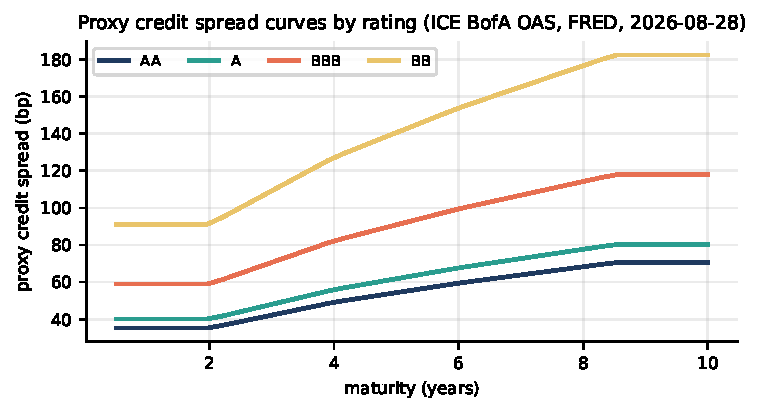
\includegraphics[width=\linewidth]{figures/fig35.pdf}
\caption{Proxy spread curves by rating on the valuation date. The BBB curve used for the counterparties runs from about 59 bp at 6 months to about 118 bp at 10 years.}
\end{figure}
{\footnotesize\setlength{\LTpre}{4pt}\setlength{\LTpost}{6pt}
\begin{longtable}{>{\raggedright\arraybackslash}p{\dimexpr 0.1579\linewidth-2\tabcolsep\relax}>{\raggedright\arraybackslash}p{\dimexpr 0.1579\linewidth-2\tabcolsep\relax}>{\raggedright\arraybackslash}p{\dimexpr 0.2895\linewidth-2\tabcolsep\relax}>{\raggedright\arraybackslash}p{\dimexpr 0.3947\linewidth-2\tabcolsep\relax}}
\toprule
\rowcolor{navy}\textbf{\textcolor{white}{Counterparty}} & \textbf{\textcolor{white}{Assumed rating}} & \textbf{\textcolor{white}{Assumed sector}} & \textbf{\textcolor{white}{Basis}} \\
\endhead
CPTY\_A & BBB & Financials (SA-CVA bucket 2) & Assumption: unrated counterparty proxied at BBB \\
\rowcolor{gray!9}CPTY\_B & BBB & Financials (SA-CVA bucket 2) & Assumption \\
CPTY\_C & BBB & Financials (SA-CVA bucket 2) & Assumption \\
\bottomrule
\end{longtable}}

The counterparty identities and ratings were not provided, so these are explicit assumptions. Because they matter more than any modelling choice, Section 8.3 reports CVA across the whole rating range so the reader can substitute the correct rating.

\subsection{Results: CVA}
\begin{figure}[H]
\centering
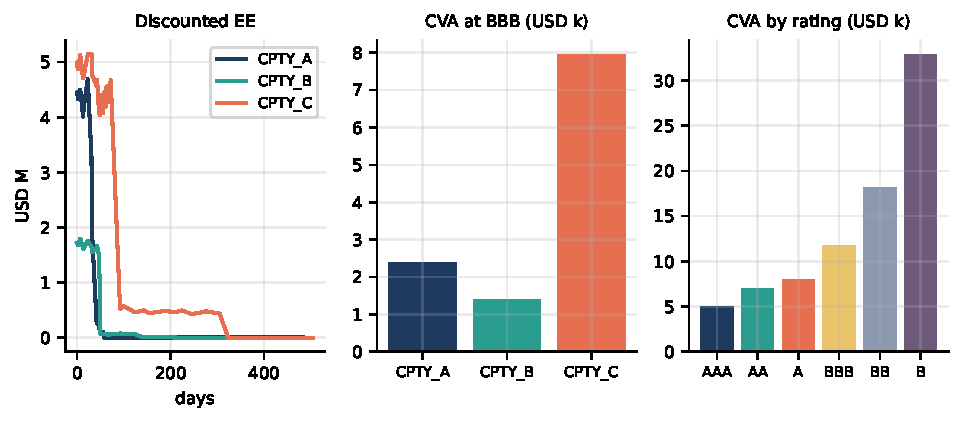
\includegraphics[width=\linewidth]{figures/fig36.pdf}
\caption{Left: expected discounted exposure by counterparty. Middle: CVA by counterparty at the BBB proxy. Right: portfolio CVA if all counterparties had the rating shown.}
\end{figure}
{\footnotesize\setlength{\LTpre}{4pt}\setlength{\LTpost}{6pt}
\begin{longtable}{>{\raggedright\arraybackslash}p{\dimexpr 0.3636\linewidth-2\tabcolsep\relax}>{\raggedright\arraybackslash}p{\dimexpr 0.3636\linewidth-2\tabcolsep\relax}>{\raggedright\arraybackslash}p{\dimexpr 0.2727\linewidth-2\tabcolsep\relax}}
\toprule
\rowcolor{navy}\textbf{\textcolor{white}{Counterparty}} & \textbf{\textcolor{white}{CVA (USD)}} & \textbf{\textcolor{white}{Share of total}} \\
\endhead
CPTY\_A & 2,400 & 20\% \\
\rowcolor{gray!9}CPTY\_B & 1,400 & 12\% \\
CPTY\_C & 7,947 & 68\% \\
\rowcolor{gray!9}Portfolio & 11,747 & 100\% \\
\bottomrule
\end{longtable}}

{\footnotesize\setlength{\LTpre}{4pt}\setlength{\LTpost}{6pt}
\begin{longtable}{>{\raggedright\arraybackslash}p{\dimexpr 0.2449\linewidth-2\tabcolsep\relax}>{\raggedright\arraybackslash}p{\dimexpr 0.4490\linewidth-2\tabcolsep\relax}>{\raggedright\arraybackslash}p{\dimexpr 0.3061\linewidth-2\tabcolsep\relax}}
\toprule
\rowcolor{navy}\textbf{\textcolor{white}{Rating}} & \textbf{\textcolor{white}{Portfolio CVA (USD)}} & \textbf{\textcolor{white}{Multiple of BBB}} \\
\endhead
AAA & 4,970 & 0.42x \\
\rowcolor{gray!9}AA & 7,028 & 0.60x \\
A & 7,997 & 0.68x \\
\rowcolor{gray!9}BBB & 11,747 & 1.00x \\
BB & 18,150 & 1.55x \\
\rowcolor{gray!9}B & 32,847 & 2.80x \\
\bottomrule
\end{longtable}}

CVA is concentrated where the exposure is: CPTY\_C carries 68\% of it. CVA scales approximately linearly with the credit spread, so the rating assumption moves the result by a factor of about 2.6 between AA and BB. The CVA figures use 5,000 scenarios (Latin Hypercube) on the brief's close-out exposure; on the uncollateralized level exposure the total is \$247,133 (Section 8.5). The SA-CVA sensitivities of Section 8.4 use 1,000 scenarios with common random numbers.

\subsection{Basel SA-CVA capital}
SA-CVA (MAR50.27 to 50.77) sets capital from the sensitivity of regulatory CVA to market risk factors. It is an adaptation of the market-risk standardised approach and needs supervisory approval, a CVA desk and monthly sensitivity calculation (MAR50.30); the figures here are therefore indicative of the requirement, not a filed number. For each risk factor k the CVA sensitivity s\_k is computed by bump-and-reprice with common random numbers, converted to a weighted sensitivity WS\_k = RW\_k x s\_k, and aggregated by bucket and risk class:

On this version the CVA sensitivities are taken on the brief's close-out exposure (1,000 scenarios, common random numbers). Equity and FX delta bumps reuse the base paths and reprice only the trades that hold the factor, exactly as for the Greeks (Section 9.4); interest-rate and volatility bumps re-simulate.

\textbf{SA-CVA capital on the two exposure definitions.} The capital is a multiple of the CVA and its sensitivities, so it follows the exposure definition: on the margined close-out exposure it is \$0.10M (RWA \$1.2M), on the uncollateralized level exposure \$2.23M (RWA \$27.8M). If no margin is ever called the second figure is the relevant one; the first applies only to a counterparty with daily variation margin at the prior-day value. Both are dominated by counterparty credit spread risk.

{\scriptsize\setlength{\LTpre}{4pt}\setlength{\LTpost}{6pt}
\begin{longtable}{>{\raggedright\arraybackslash}p{\dimexpr 0.3846\linewidth-2\tabcolsep\relax}>{\raggedright\arraybackslash}p{\dimexpr 0.2821\linewidth-2\tabcolsep\relax}>{\raggedright\arraybackslash}p{\dimexpr 0.3333\linewidth-2\tabcolsep\relax}}
\toprule
\rowcolor{navy}\textbf{\textcolor{white}{Risk class}} & \textbf{\textcolor{white}{Close-out exposure (USD)}} & \textbf{\textcolor{white}{Uncollateralized level exposure (USD)}} \\
\endhead
ir delta & 775 & 74,837 \\
\rowcolor{gray!9}ir vega & 5,284 & 253 \\
fx delta & 95 & 2,351 \\
\rowcolor{gray!9}fx vega & 0 & 0 \\
ccs delta & 85,198 & 2,032,731 \\
\rowcolor{gray!9}eq delta & 2,068 & 110,371 \\
eq vega & 3,256 & 6,278 \\
\rowcolor{gray!9}Total SA-CVA capital (m\_CVA = 1) & 96,675 & 2,226,821 \\
Risk-weighted assets (12.5 x capital) & 1,208,436 & 27,835,265 \\
\rowcolor{gray!9}CVA in the sensitivity base run & 11,731 & 246,650 \\
\bottomrule
\end{longtable}}

{\fontsize{7.2}{8.8}\selectfont
\begin{verbatim}
K_b = sqrt( sum_k WS_k^2 + sum_{k!=l} rho_kl WS_k WS_l )        S_b = clip( sum_k WS_k, -K_b, +K_b )
K   = m_CVA * sqrt( sum_b K_b^2 + sum_{b!=c} gamma_bc S_b S_c )
Capital = sum over classes of ( K_delta + K_vega );   RWA = 12.5 * Capital
\end{verbatim}}
Risk classes present in the book, the shift used for each sensitivity and the Basel parameters applied:

{\scriptsize\setlength{\LTpre}{4pt}\setlength{\LTpost}{6pt}
\begin{longtable}{>{\raggedright\arraybackslash}p{\dimexpr 0.2025\linewidth-2\tabcolsep\relax}>{\raggedright\arraybackslash}p{\dimexpr 0.3797\linewidth-2\tabcolsep\relax}>{\raggedright\arraybackslash}p{\dimexpr 0.2152\linewidth-2\tabcolsep\relax}>{\raggedright\arraybackslash}p{\dimexpr 0.2025\linewidth-2\tabcolsep\relax}}
\toprule
\rowcolor{navy}\textbf{\textcolor{white}{Risk class}} & \textbf{\textcolor{white}{Risk factors and shift}} & \textbf{\textcolor{white}{Risk weight}} & \textbf{\textcolor{white}{Correlation}} \\
\endhead
Interest rate delta (USD) & USD risk-free yield at 1, 2, 5, 10, 30y; +1bp with triangular weights & 1.11\%, 0.93\%, 0.74\%, 0.74\%, 0.74\% & Tenor matrix 31-91\% (Table 4) \\
\rowcolor{gray!9}Interest rate vega (USD) & All USD rate volatilities, +1\% relative & 100\% & Single factor \\
FX delta (USDJPY) & USDJPY spot, +1\% relative & 11\% & Single factor; cross-bucket 0.6 \\
\rowcolor{gray!9}FX vega & USDJPY volatility, +1\% relative & 100\% & Single factor \\
Counterparty credit spread & Each counterparty at 0.5, 1, 3, 5, 10y; +1bp & 5\% (financials, investment grade) & Tenor 0.9 x name 0.5 (unrelated) \\
\rowcolor{gray!9}Equity delta & All names in an equity bucket, +1\% relative spot & 30-55\% by bucket & Cross-bucket 0.15 \\
Equity vega & All volatilities in a bucket, +1\% relative & 78\% large cap, 100\% small cap & Cross-bucket 0.15 \\
\rowcolor{gray!9}Reference credit, commodity & None: no such drivers of exposure & - & - \\
\bottomrule
\end{longtable}}

Equity names are assigned to Basel buckets by size (market capitalisation of at least USD 2 billion), region (advanced versus emerging economy) and sector, using yfinance data: bucket 1: 1 names, bucket 4: 2 names, bucket 5: 13 names, bucket 6: 6 names, bucket 7: 2 names, bucket 8: 13 names.

\begin{figure}[H]
\centering
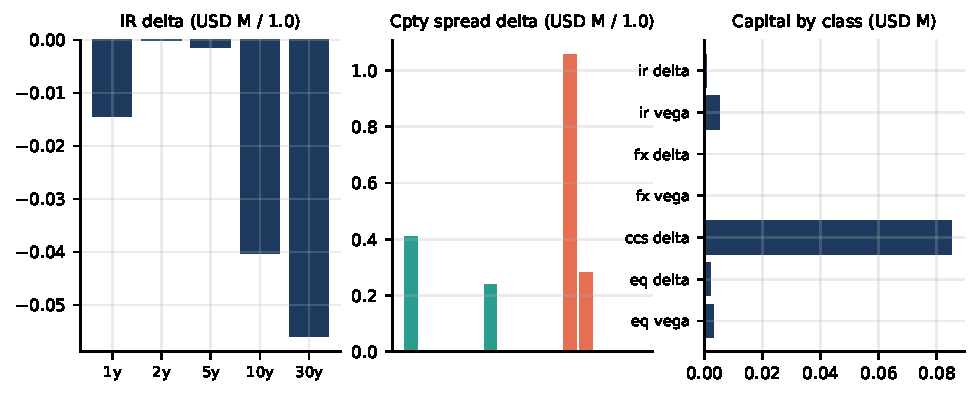
\includegraphics[width=\linewidth]{figures/fig37.pdf}
\caption{Left: CVA sensitivity to a 1bp rise in USD yields at each SA-CVA tenor. Middle: sensitivity of CVA to the counterparty credit spreads (three counterparties by five tenors). Right: SA-CVA capital by risk class.}
\end{figure}
{\footnotesize\setlength{\LTpre}{4pt}\setlength{\LTpost}{6pt}
\begin{longtable}{>{\raggedright\arraybackslash}p{\dimexpr 0.6667\linewidth-2\tabcolsep\relax}>{\raggedright\arraybackslash}p{\dimexpr 0.3333\linewidth-2\tabcolsep\relax}}
\toprule
\rowcolor{navy}\textbf{\textcolor{white}{Risk class}} & \textbf{\textcolor{white}{Capital K (USD)}} \\
\endhead
ir delta & 775 \\
\rowcolor{gray!9}ir vega & 5,284 \\
fx delta & 95 \\
\rowcolor{gray!9}fx vega & 0 \\
ccs delta & 85,198 \\
\rowcolor{gray!9}eq delta & 2,068 \\
eq vega & 3,256 \\
\rowcolor{gray!9}Total SA-CVA capital requirement (m\_CVA = 1) & 96,675 \\
Risk-weighted assets (12.5 x capital) & 1,208,436 \\
\rowcolor{gray!9}Total if the pre-2023 multiplier m\_CVA = 1.25 applied & 120,844 \\
\bottomrule
\end{longtable}}

The requirement is dominated by ccs delta (88\% of the total), as is typical: a 5\% risk weight on credit spreads is large relative to a 100 bp spread level, so the capital charge is a multiple of the CVA itself. Interest rate, FX and equity classes are comparatively small. The multiplier m\_CVA is 1 in the framework in force from 2023 (it was 1.25 in the original 2017 text); both are shown.

\subsection{DVA and FVA}
CVA prices the counterparty's default. Two further adjustments complete the xVA picture. \textbf{DVA} is its mirror image: the bank's own default probability applied to what we owe the counterparty, the negative exposure. \textbf{FVA} is the cost of funding the positive exposure (funding cost, FCA) less the benefit of the negative exposure (funding benefit, FBA) at a funding spread. With EPE and ENE the discounted expected positive and negative exposures:

{\fontsize{7.2}{8.8}\selectfont
\begin{verbatim}
DVA = LGD_own * sum 0.5 (ENE_{i-1} + ENE_i) * PD_own(t_{i-1}, t_i)
FCA = sum s_f(t_i) dt_i * 0.5 (EPE_{i-1} + EPE_i)       FBA = same with ENE       FVA = FCA - FBA
\end{verbatim}}
Both need inputs that are not in the data: Capitolis' own credit and its funding spread. They are assumptions: own credit is proxied by the same BBB bond-index curve as the counterparties (an unrated fintech is at best a BBB proxy) and the funding spread is set equal to the own credit spread, the standard symmetric assumption. Under that assumption the funding benefit and DVA capture the same economic benefit, so the figure that avoids double counting is CVA - DVA + FCA. The Basel capital framework ignores DVA. The results depend on these assumptions and are shown with their sensitivity to own credit quality.

\textbf{Close-out exposure (headline)}

{\scriptsize\setlength{\LTpre}{4pt}\setlength{\LTpost}{6pt}
\begin{longtable}{>{\raggedright\arraybackslash}p{\dimexpr 0.1579\linewidth-2\tabcolsep\relax}>{\raggedright\arraybackslash}p{\dimexpr 0.1184\linewidth-2\tabcolsep\relax}>{\raggedright\arraybackslash}p{\dimexpr 0.1184\linewidth-2\tabcolsep\relax}>{\raggedright\arraybackslash}p{\dimexpr 0.1184\linewidth-2\tabcolsep\relax}>{\raggedright\arraybackslash}p{\dimexpr 0.1184\linewidth-2\tabcolsep\relax}>{\raggedright\arraybackslash}p{\dimexpr 0.1842\linewidth-2\tabcolsep\relax}>{\raggedright\arraybackslash}p{\dimexpr 0.1842\linewidth-2\tabcolsep\relax}}
\toprule
\rowcolor{navy}\textbf{\textcolor{white}{Netting set}} & \textbf{\textcolor{white}{CVA}} & \textbf{\textcolor{white}{DVA}} & \textbf{\textcolor{white}{FCA}} & \textbf{\textcolor{white}{FBA}} & \textbf{\textcolor{white}{FVA = FCA - FBA}} & \textbf{\textcolor{white}{CVA - DVA + FVA}} \\
\endhead
CPTY\_A & \$2k & \$2k & \$2k & \$2k & \$0k & \$0k \\
\rowcolor{gray!9}CPTY\_B & \$1k & \$1k & \$1k & \$1k & \$0k & \$0k \\
CPTY\_C & \$8k & \$8k & \$8k & \$8k & \$0k & \$1k \\
\rowcolor{gray!9}Total & \$12k & \$11k & \$12k & \$11k & \$1k & \$1k \\
\bottomrule
\end{longtable}}

\textbf{Uncollateralized level exposure (secondary)}

{\scriptsize\setlength{\LTpre}{4pt}\setlength{\LTpost}{6pt}
\begin{longtable}{>{\raggedright\arraybackslash}p{\dimexpr 0.1579\linewidth-2\tabcolsep\relax}>{\raggedright\arraybackslash}p{\dimexpr 0.1184\linewidth-2\tabcolsep\relax}>{\raggedright\arraybackslash}p{\dimexpr 0.1184\linewidth-2\tabcolsep\relax}>{\raggedright\arraybackslash}p{\dimexpr 0.1184\linewidth-2\tabcolsep\relax}>{\raggedright\arraybackslash}p{\dimexpr 0.1184\linewidth-2\tabcolsep\relax}>{\raggedright\arraybackslash}p{\dimexpr 0.1842\linewidth-2\tabcolsep\relax}>{\raggedright\arraybackslash}p{\dimexpr 0.1842\linewidth-2\tabcolsep\relax}}
\toprule
\rowcolor{navy}\textbf{\textcolor{white}{Netting set}} & \textbf{\textcolor{white}{CVA}} & \textbf{\textcolor{white}{DVA}} & \textbf{\textcolor{white}{FCA}} & \textbf{\textcolor{white}{FBA}} & \textbf{\textcolor{white}{FVA = FCA - FBA}} & \textbf{\textcolor{white}{CVA - DVA + FVA}} \\
\endhead
CPTY\_A & \$7k & \$3k & \$7k & \$3k & \$4k & \$7k \\
\rowcolor{gray!9}CPTY\_B & \$4k & \$2k & \$4k & \$2k & \$2k & \$4k \\
CPTY\_C & \$237k & \$3k & \$237k & \$3k & \$234k & \$468k \\
\rowcolor{gray!9}Total & \$247k & \$8k & \$248k & \$8k & \$240k & \$480k \\
\bottomrule
\end{longtable}}

\begin{figure}[H]
\centering
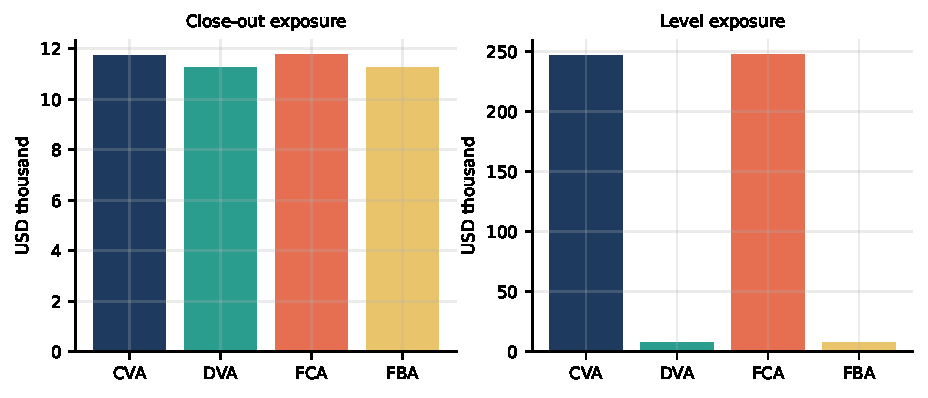
\includegraphics[width=\linewidth]{figures/fig38.pdf}
\caption{xVA components, total over the three netting sets, on the two exposure definitions.}
\end{figure}
\begin{figure}[H]
\centering
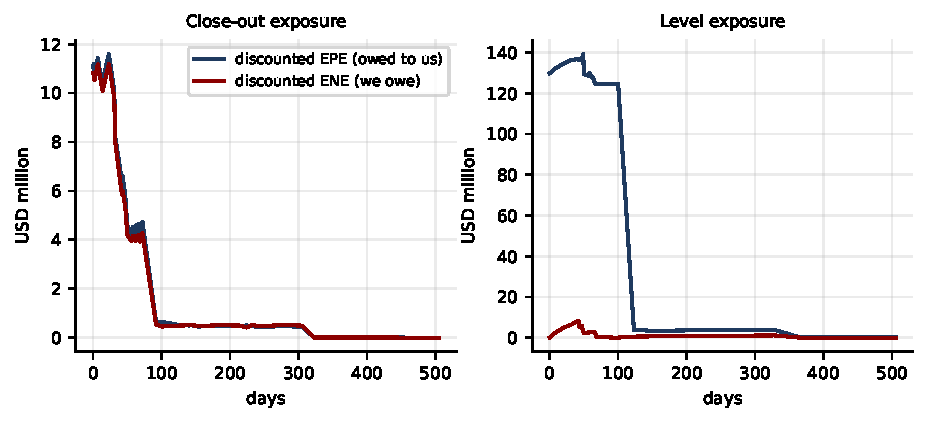
\includegraphics[width=\linewidth]{figures/fig39.pdf}
\caption{Discounted expected positive and negative exposure, summed over counterparties. DVA and the funding benefit come from the negative side.}
\end{figure}
\textbf{Sensitivity to the assumed own credit quality} (close-out exposure; the funding spread is set equal to the own credit spread):

{\scriptsize\setlength{\LTpre}{4pt}\setlength{\LTpost}{6pt}
\begin{longtable}{>{\raggedright\arraybackslash}p{\dimexpr 0.1884\linewidth-2\tabcolsep\relax}>{\raggedright\arraybackslash}p{\dimexpr 0.1304\linewidth-2\tabcolsep\relax}>{\raggedright\arraybackslash}p{\dimexpr 0.1304\linewidth-2\tabcolsep\relax}>{\raggedright\arraybackslash}p{\dimexpr 0.1304\linewidth-2\tabcolsep\relax}>{\raggedright\arraybackslash}p{\dimexpr 0.1304\linewidth-2\tabcolsep\relax}>{\raggedright\arraybackslash}p{\dimexpr 0.2899\linewidth-2\tabcolsep\relax}}
\toprule
\rowcolor{navy}\textbf{\textcolor{white}{Own rating proxy}} & \textbf{\textcolor{white}{DVA}} & \textbf{\textcolor{white}{FCA}} & \textbf{\textcolor{white}{FBA}} & \textbf{\textcolor{white}{FVA}} & \textbf{\textcolor{white}{CVA - DVA + FCA (no overlap)}} \\
\endhead
AA & \$7k & \$7k & \$7k & \$0k & \$12k \\
\rowcolor{gray!9}A & \$8k & \$8k & \$8k & \$0k & \$12k \\
BBB & \$11k & \$12k & \$11k & \$1k & \$12k \\
\rowcolor{gray!9}BB & \$17k & \$18k & \$17k & \$1k & \$13k \\
\bottomrule
\end{longtable}}

\textbf{Reading the table.} On the margined close-out exposure the total CVA is \$12k and DVA \$11k, so the net credit charge is \$1k; funding costs \$1k (FCA \$12k less FBA \$11k). On the close-out definition the positive and negative sides are nearly symmetric, because both are 10-day moves around a margined start, so CVA and DVA almost cancel and the funding terms are small. On the level exposure CVA is \$247k and DVA \$8k: the difference from the close-out figures is the whole mark-to-market that margin would otherwise cover, and the asymmetry comes from the book being mostly in our favour (CPTY\_C's bond forward), which makes the positive exposure, and therefore CVA and FCA, much larger than the negative exposure that drives DVA and FBA.

\subsection{SA-CCR exposure at default}
The Basel standardised approach for counterparty credit risk (SA-CCR, CRE52) gives a regulatory exposure at default, EAD = 1.4 x (replacement cost + multiplier x add-on), for each uncollateralized netting set. It is built in exposure/sa\_ccr.py for the asset classes present in the book (interest rate for the Treasury forwards and bond TRS, equity for the equity TRS; no FX, credit or commodity trades), validated against hand calculations of the supervisory duration, maturity factor, bucket and entity aggregation and the multiplier.

{\scriptsize\setlength{\LTpre}{4pt}\setlength{\LTpost}{6pt}
\begin{longtable}{>{\raggedright\arraybackslash}p{\dimexpr 0.1071\linewidth-2\tabcolsep\relax}>{\raggedright\arraybackslash}p{\dimexpr 0.1071\linewidth-2\tabcolsep\relax}>{\raggedright\arraybackslash}p{\dimexpr 0.1190\linewidth-2\tabcolsep\relax}>{\raggedright\arraybackslash}p{\dimexpr 0.1071\linewidth-2\tabcolsep\relax}>{\raggedright\arraybackslash}p{\dimexpr 0.1071\linewidth-2\tabcolsep\relax}>{\raggedright\arraybackslash}p{\dimexpr 0.0952\linewidth-2\tabcolsep\relax}>{\raggedright\arraybackslash}p{\dimexpr 0.1071\linewidth-2\tabcolsep\relax}>{\raggedright\arraybackslash}p{\dimexpr 0.1071\linewidth-2\tabcolsep\relax}>{\raggedright\arraybackslash}p{\dimexpr 0.1429\linewidth-2\tabcolsep\relax}}
\toprule
\rowcolor{navy}\textbf{\textcolor{white}{Netting set}} & \textbf{\textcolor{white}{Net MtM V}} & \textbf{\textcolor{white}{Replacement cost}} & \textbf{\textcolor{white}{Add-on, rates}} & \textbf{\textcolor{white}{Add-on, equity}} & \textbf{\textcolor{white}{Multiplier}} & \textbf{\textcolor{white}{PFE}} & \textbf{\textcolor{white}{EAD}} & \textbf{\textcolor{white}{MC MPE99 (close-out)}} \\
\endhead
CPTY\_A & \$3.6M & \$3.6M & \$1.1M & \$15.7M & 1.00 & \$16.7M & \$28.4M & \$25.9M \\
\rowcolor{gray!9}CPTY\_B & \$1.0M & \$1.0M & \$1.8M & \$7.3M & 1.00 & \$9.1M & \$14.0M & \$9.6M \\
CPTY\_C & \$125.1M & \$125.1M & \$17.8M & \$12.7M & 1.00 & \$30.5M & \$217.8M & \$29.6M \\
\rowcolor{gray!9}Total & \$129.6M & \$129.6M &  &  &  & \$56.3M & \$260.3M & \$51.0M \\
\bottomrule
\end{longtable}}

{\small SA-CCR is not comparable to the Monte Carlo maximum PFE99 because it is a different quantity: its replacement cost is today's full mark-to-market and its add-on is a one-year supervisory approximation, whereas the close-out MPE99 measures the 10-day move of a margined position. It is included as the regulatory view of the same book and as an independent order-of-magnitude check on the add-on: for the equity netting sets the SA-CCR PFE is of the same order as the Monte Carlo level-exposure MPE, and for CPTY\_C the replacement cost of the 500M bond forward dominates.}

\subsection{CVA walk-through and set-up for the next session}
This section walks through the CVA calculation step by step for one netting set, CPTY\_C, on the close-out exposure, with the numbers behind each column, and closes with the questions to settle at the next session.

\textbf{The formula.} Credit valuation adjustment is the expected loss from a counterparty default, priced under the risk-neutral measure (Basel MAR50.32):

{\fontsize{7.2}{8.8}\selectfont
\begin{verbatim}
CVA = LGD * sum_i  0.5 * ( DEE(t_{i-1}) + DEE(t_i) ) * PD(t_{i-1}, t_i)
DEE(t)   = E[ D(t) * exposure(t) ]           expected discounted exposure, D = pathwise discount factor
PD(a,b)  = Q(a) - Q(b),  Q(t) = exp( -s(t) t / LGD )      default probability from the credit spread s
\end{verbatim}}
Inputs, in the order they enter: (1) the exposure profile from the simulation (Section 7.1), discounted along each path with the simulated short rate; (2) the counterparty's credit spread curve, here a proxy (ICE BofA BBB option-adjusted spreads, 59 bp at 1 year and 91 bp at 5 years) because no CDS was available and the counterparties are anonymised; (3) a loss given default of 60\% (recovery 40\%); (4) the assumption that exposure and default are independent (no wrong-way risk).

\textbf{CPTY\_C, close-out exposure (headline).} Selected dates spread over the life of the book; the last row sums all intervals:

{\scriptsize\setlength{\LTpre}{4pt}\setlength{\LTpost}{6pt}
\begin{longtable}{>{\raggedright\arraybackslash}p{\dimexpr 0.1475\linewidth-2\tabcolsep\relax}>{\raggedright\arraybackslash}p{\dimexpr 0.1475\linewidth-2\tabcolsep\relax}>{\raggedright\arraybackslash}p{\dimexpr 0.1475\linewidth-2\tabcolsep\relax}>{\raggedright\arraybackslash}p{\dimexpr 0.1639\linewidth-2\tabcolsep\relax}>{\raggedright\arraybackslash}p{\dimexpr 0.1639\linewidth-2\tabcolsep\relax}>{\raggedright\arraybackslash}p{\dimexpr 0.2295\linewidth-2\tabcolsep\relax}}
\toprule
\rowcolor{navy}\textbf{\textcolor{white}{Date (years)}} & \textbf{\textcolor{white}{DEE}} & \textbf{\textcolor{white}{Spread (bp)}} & \textbf{\textcolor{white}{Survival Q(t)}} & \textbf{\textcolor{white}{Interval PD}} & \textbf{\textcolor{white}{Contribution to CVA}} \\
\endhead
0.00 & \$5,004k & 59 & 1.0000 & 0.003\% & \$0k \\
\rowcolor{gray!9}0.04 & \$4,735k & 59 & 0.9996 & 0.003\% & \$0k \\
0.08 & \$5,142k & 59 & 0.9992 & 0.022\% & \$1k \\
\rowcolor{gray!9}0.16 & \$4,455k & 59 & 0.9984 & 0.005\% & \$0k \\
0.25 & \$522k & 59 & 0.9975 & 0.054\% & \$1k \\
\rowcolor{gray!9}0.34 & \$462k & 59 & 0.9967 & 0.062\% & \$0k \\
0.42 & \$441k & 59 & 0.9959 & 0.032\% & \$0k \\
\rowcolor{gray!9}0.50 & \$480k & 59 & 0.9951 & 0.080\% & \$0k \\
0.58 & \$466k & 59 & 0.9943 & 0.078\% & \$0k \\
\rowcolor{gray!9}0.67 & \$427k & 59 & 0.9935 & 0.032\% & \$0k \\
0.75 & \$479k & 59 & 0.9927 & 0.003\% & \$0k \\
\rowcolor{gray!9}1.00 & \$0k & 59 & 0.9902 & 0.099\% & \$0k \\
1.14 & \$0k & 60 & 0.9887 & 0.148\% & \$0k \\
\rowcolor{gray!9}1.38 & \$0k & 61 & 0.9860 & 0.275\% & \$0k \\
All 41 intervals &  &  &  & 1.40\% & \$8k \\
\bottomrule
\end{longtable}}

\textbf{CPTY\_C, uncollateralized level exposure.} Selected dates spread over the life of the book; the last row sums all intervals:

{\scriptsize\setlength{\LTpre}{4pt}\setlength{\LTpost}{6pt}
\begin{longtable}{>{\raggedright\arraybackslash}p{\dimexpr 0.1475\linewidth-2\tabcolsep\relax}>{\raggedright\arraybackslash}p{\dimexpr 0.1475\linewidth-2\tabcolsep\relax}>{\raggedright\arraybackslash}p{\dimexpr 0.1475\linewidth-2\tabcolsep\relax}>{\raggedright\arraybackslash}p{\dimexpr 0.1639\linewidth-2\tabcolsep\relax}>{\raggedright\arraybackslash}p{\dimexpr 0.1639\linewidth-2\tabcolsep\relax}>{\raggedright\arraybackslash}p{\dimexpr 0.2295\linewidth-2\tabcolsep\relax}}
\toprule
\rowcolor{navy}\textbf{\textcolor{white}{Date (years)}} & \textbf{\textcolor{white}{DEE}} & \textbf{\textcolor{white}{Spread (bp)}} & \textbf{\textcolor{white}{Survival Q(t)}} & \textbf{\textcolor{white}{Interval PD}} & \textbf{\textcolor{white}{Contribution to CVA}} \\
\endhead
0.00 & \$125,006k & 59 & 1.0000 & 0.003\% & \$2k \\
\rowcolor{gray!9}0.04 & \$125,168k & 59 & 0.9996 & 0.003\% & \$2k \\
0.08 & \$125,348k & 59 & 0.9992 & 0.022\% & \$16k \\
\rowcolor{gray!9}0.16 & \$125,913k & 59 & 0.9984 & 0.005\% & \$4k \\
0.25 & \$123,981k & 59 & 0.9975 & 0.054\% & \$40k \\
\rowcolor{gray!9}0.34 & \$2,903k & 59 & 0.9967 & 0.062\% & \$23k \\
0.42 & \$3,068k & 59 & 0.9959 & 0.032\% & \$1k \\
\rowcolor{gray!9}0.50 & \$3,207k & 59 & 0.9951 & 0.080\% & \$2k \\
0.58 & \$3,316k & 59 & 0.9943 & 0.078\% & \$2k \\
\rowcolor{gray!9}0.67 & \$3,433k & 59 & 0.9935 & 0.032\% & \$1k \\
0.75 & \$3,537k & 59 & 0.9927 & 0.003\% & \$0k \\
\rowcolor{gray!9}1.00 & \$0k & 59 & 0.9902 & 0.099\% & \$1k \\
1.14 & \$0k & 60 & 0.9887 & 0.148\% & \$0k \\
\rowcolor{gray!9}1.38 & \$0k & 61 & 0.9860 & 0.275\% & \$0k \\
All 41 intervals &  &  &  & 1.40\% & \$237k \\
\bottomrule
\end{longtable}}

\textbf{Reading the numbers.} The CVA is small relative to the exposure because the default probability over a year or two is small (a BBB spread of about 100bp gives roughly 1.7\% a year at 60\% LGD) and because the exposure runs off quickly as trades mature. On the close-out definition the total CVA for the three netting sets is \$12k; on the uncollateralized level exposure it is \$247k, larger because the level exposure keeps the whole mark-to-market at risk (for CPTY\_C the 500M bond forward: \$237k against \$8k). The close-out figure is what a margined counterparty would cost; the level figure is the price if no margin were ever called.

\textbf{To settle at the next session.}

\begin{itemize}
\item \textbf{Exposure definition for CVA.} Confirm that CVA should be on the brief's margined close-out exposure, with the uncollateralized figure as an upper bound, or whether Capitolis prices CVA on the level exposure.
\item \textbf{Counterparty credit.} Real ratings or CDS for CPTY\_A, CPTY\_B and CPTY\_C (the BBB proxy drives everything; the sensitivity of the total to the rating is in the table of Section 8.3). Whether a sector or region adjustment is wanted.
\item \textbf{Capitolis' own credit and funding.} DVA and FVA are computed on assumptions (own credit BBB, funding spread equal to own spread); they need a Capitolis curve, and a decision on whether DVA is recognised at all (Basel CVA capital ignores it).
\item \textbf{Wrong-way risk.} The independence of exposure and default is assumed. Is a dependence model wanted, and for which counterparties (an equity swap counterparty that is itself an equity-sensitive institution)?
\item \textbf{Capital.} SA-CVA is computed with the m\_CVA = 1 multiplier; agree whether the reduced basic approach (BA-CVA) or the standardised approach is the reference, and whether hedges should be included.
\item \textbf{Margin terms.} Threshold, minimum transfer amount and initial margin are not in the data; the CVA under those terms would sit between the two exposure definitions shown.
\end{itemize}
\subsection{Assumptions and limitations of the CVA work}
\begin{itemize}
\item \textbf{Counterparty ratings are assumed} (BBB financials). CVA and the credit-spread capital scale with this assumption; Section 8.3 shows the range.
\item \textbf{Spreads are bond-index proxies}, not CDS: the maturity shape is common to all ratings, and the indices are US corporate spreads regardless of counterparty region or sector.
\item \textbf{Independence and margin.} Headline CVA is unilateral, with exposure and default independent (no wrong-way risk). The two exposure definitions bracket the truth: the close-out exposure assumes daily variation margin at the prior-day value, the level exposure assumes none. Threshold, minimum transfer amount and initial margin are not in the data. DVA and FVA rest on an assumed own credit and funding spread.
\item \textbf{Interest rate risk:} SA-CVA interest-rate delta and vega are computed for the USD curve. The JPY rate is simulated but only drives the drift of JPY-listed names and USDJPY, and no trade is discounted on JPY, so no JPY rate class is needed; inflation risk factors are omitted (no inflation exposure).
\item \textbf{Sensitivities are one-sided bumps} with common random numbers, not adjoint sensitivities; vega shifts apply to the volatilities driving the simulated paths (the trades contain no options, so there are no option-pricing volatilities).
\item \textbf{Parameters} are transcribed from the BIS text (July 2020 revisions); the vega risk weights follow the 100\% and 78\% values in that text. Regulatory use requires supervisory approval and validation of the sensitivity calculation.
\item The Basel Basic Approach (BA-CVA) is not computed; it needs only counterparty exposure and maturity and is the natural fallback if SA-CVA approval is not held.
\end{itemize}
\subsection{Extra credit: a risky-bond sample trade}
\textbf{Extra credit: risky bonds.} The brief invites risky bonds and CDS data for new sample trades. No CDS quotes were obtainable, so the issuer credit curve is a proxy built the same way as the counterparty spreads: ICE BofA BBB option-adjusted spreads (0.5y 59bp, 1.0y 59bp, 3.0y 71bp, 5.0y 91bp, 10.0y 118bp) with the pricing library's credit-triangle survival curve (recovery 40\%). A sample long forward on a 5\% BBB corporate bond (25M notional, forward date 2027-02-26; trade\_data/samples/, not part of the ESF book) is priced with and without issuer credit, and simulated with the issuer curve re-anchored at every node with the same term structure (deterministic spreads).

{\scriptsize\setlength{\LTpre}{4pt}\setlength{\LTpost}{6pt}
\begin{longtable}{>{\raggedright\arraybackslash}p{\dimexpr 0.4545\linewidth-2\tabcolsep\relax}>{\raggedright\arraybackslash}p{\dimexpr 0.2424\linewidth-2\tabcolsep\relax}>{\raggedright\arraybackslash}p{\dimexpr 0.3030\linewidth-2\tabcolsep\relax}}
\toprule
\rowcolor{navy}\textbf{\textcolor{white}{Quantity}} & \textbf{\textcolor{white}{Risk-free bond}} & \textbf{\textcolor{white}{Risky bond (issuer credit)}} \\
\endhead
t = 0 NPV of the forward & 653,843 & -280,309 \\
\rowcolor{gray!9}Forward clean price & 102.6666 & 98.8568 \\
Issuer credit charge at t = 0 & - & 934,152 \\
\rowcolor{gray!9}CS01 (NPV change per +1bp of issuer spread) & - & -10,998 \\
Close-out MPE99 (counterparty exposure) & \$0.5M & \$0.5M \\
\rowcolor{gray!9}Peak level PFE99 (uncollateralized) & \$2.1M & \$1.3M \\
\bottomrule
\end{longtable}}

{\small Two things are distinct and should not be confused: the issuer credit charge, which is the credit risk of the bond's issuer and lowers the value of the forward, and the counterparty CVA on the trade, which is the credit risk of the other party and is computed as in Section 8. What is still missing is issuer credit as a stochastic factor (spreads are deterministic here) and CDS instruments themselves, for which the pricing library has no pricer.}

\clearpage
\section{Sensitivities (Greeks)}
Capitolis asked for exposure profiles together with efficient Greeks across scenarios, aggregated by netting set. This section delivers both levels: (i) the Greeks of the book's value today, by trade and netting set, and (ii) the sensitivities of the exposure measures themselves, EE, median PFE and PFE99, at every simulation date. Every number comes from the same pricers and simulated paths as Section 7.

\subsection{Definitions and method}
\begin{itemize}
\item \textbf{Delta} to an equity or to USDJPY: change per +1\% relative move of the spot. \textbf{Gamma}: change in that delta, [M(+1\%) - 2 M + M(-1\%)]. \textbf{DV01}: change per +1bp in USD zero rates, parallel and bucketed at 0.25, 0.5, 1, 2, 3, 5, 10 and 30 years (triangular weights that sum exactly to the parallel shift). \textbf{Vega}: change per +1\% relative shift of the volatility of the USD rate, of USDJPY and of all equities.
\item \textbf{Bump-and-reprice with common random numbers} (the same Latin Hypercube draws in base and bumped runs): the difference is then sensitivity, not Monte Carlo noise. It works on the pricers as a black box, and it applies equally to quantile measures such as PFE99, which have no simple pathwise derivative. Its accuracy compared with the pathwise estimator is shown in Section 11.6.
\item \textbf{Efficiency.} A bump of an equity or of USDJPY rescales every simulated path exactly (the GBM drift does not depend on the spot level), so no re-simulation is needed: the existing paths are reused with the spot multiplied and only the trades holding that factor are repriced, all bumps in one process pool. Rate and volatility bumps change the paths themselves, so they are re-simulated with the same random numbers.
\item Exposure Greeks are computed at N = 1,000 scenarios (Latin Hypercube), on the brief's close-out exposure, on the pillar date grid with the t - 1bd and t + 10bd nodes.
\end{itemize}
Sign convention: Capitolis is strictly the seller on these trades, and the equity swaps are of type pay-equity (we pay the equity return and receive funding), so equity deltas are negative: our value rises when the shares fall.

\subsection{Book Greeks today}
{\scriptsize\setlength{\LTpre}{4pt}\setlength{\LTpost}{6pt}
\begin{longtable}{>{\raggedright\arraybackslash}p{\dimexpr 0.1348\linewidth-2\tabcolsep\relax}>{\raggedright\arraybackslash}p{\dimexpr 0.1573\linewidth-2\tabcolsep\relax}>{\raggedright\arraybackslash}p{\dimexpr 0.1685\linewidth-2\tabcolsep\relax}>{\raggedright\arraybackslash}p{\dimexpr 0.1236\linewidth-2\tabcolsep\relax}>{\raggedright\arraybackslash}p{\dimexpr 0.1461\linewidth-2\tabcolsep\relax}>{\raggedright\arraybackslash}p{\dimexpr 0.1461\linewidth-2\tabcolsep\relax}>{\raggedright\arraybackslash}p{\dimexpr 0.1236\linewidth-2\tabcolsep\relax}}
\toprule
\rowcolor{navy}\textbf{\textcolor{white}{Netting set}} & \textbf{\textcolor{white}{NPV}} & \textbf{\textcolor{white}{Equity delta (per +1\%)}} & \textbf{\textcolor{white}{Equity gamma}} & \textbf{\textcolor{white}{FX delta (per +1\%)}} & \textbf{\textcolor{white}{DV01 (per +1bp)}} & \textbf{\textcolor{white}{Rate gamma}} \\
\endhead
CPTY\_A & 3,572,955 & -2,254,257 & 0 & 0 & 31,203 & -16 \\
\rowcolor{gray!9}CPTY\_B & 1,145,975 & -961,146 & 0 & 416,550 & -3,663 & 6 \\
CPTY\_C & 125,116,984 & -1,240,431 & 0 & 0 & 594,443 & -1,205 \\
\rowcolor{gray!9}Portfolio & 129,835,914 & -4,455,835 & 0 & 416,550 & 621,983 & -1,215 \\
\bottomrule
\end{longtable}}

All values in USD. The equity and bond trades are linear in the equity spot, so equity and FX gamma are zero to rounding; rate gamma is small. The DV01 is dominated by the CPTY\_C bond forward. The largest deltas and the bucketed DV01s:

\begin{figure}[H]
\centering
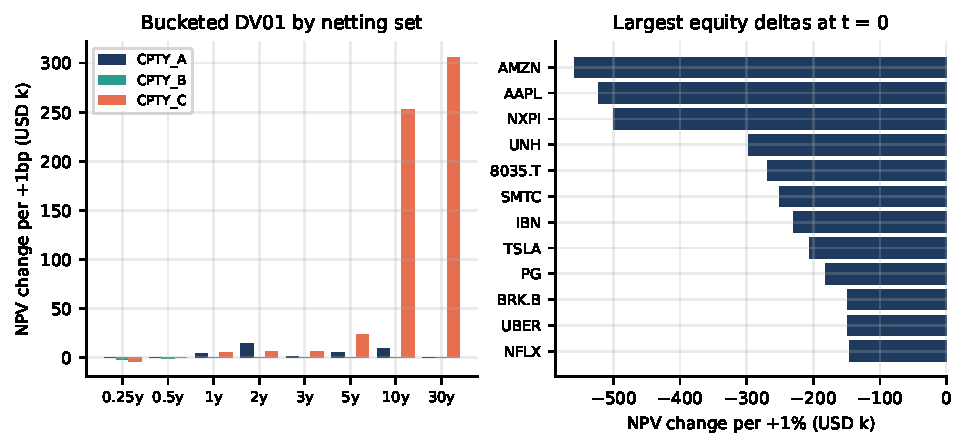
\includegraphics[width=\linewidth]{figures/fig40.pdf}
\caption{Left: DV01 by netting set and tenor. Right: the twelve largest equity deltas at t = 0.}
\end{figure}
{\scriptsize\setlength{\LTpre}{4pt}\setlength{\LTpost}{6pt}
\begin{longtable}{>{\raggedright\arraybackslash}p{\dimexpr 0.1111\linewidth-2\tabcolsep\relax}>{\raggedright\arraybackslash}p{\dimexpr 0.1111\linewidth-2\tabcolsep\relax}>{\raggedright\arraybackslash}p{\dimexpr 0.1111\linewidth-2\tabcolsep\relax}>{\raggedright\arraybackslash}p{\dimexpr 0.1111\linewidth-2\tabcolsep\relax}>{\raggedright\arraybackslash}p{\dimexpr 0.1111\linewidth-2\tabcolsep\relax}>{\raggedright\arraybackslash}p{\dimexpr 0.1111\linewidth-2\tabcolsep\relax}>{\raggedright\arraybackslash}p{\dimexpr 0.1111\linewidth-2\tabcolsep\relax}>{\raggedright\arraybackslash}p{\dimexpr 0.1111\linewidth-2\tabcolsep\relax}>{\raggedright\arraybackslash}p{\dimexpr 0.1111\linewidth-2\tabcolsep\relax}}
\toprule
\rowcolor{navy}\textbf{\textcolor{white}{Netting set}} & \textbf{\textcolor{white}{0.25y}} & \textbf{\textcolor{white}{0.5y}} & \textbf{\textcolor{white}{1y}} & \textbf{\textcolor{white}{2y}} & \textbf{\textcolor{white}{3y}} & \textbf{\textcolor{white}{5y}} & \textbf{\textcolor{white}{10y}} & \textbf{\textcolor{white}{30y}} \\
\endhead
CPTY\_A & -567 & 83 & 3,717 & 13,866 & 399 & 4,901 & 8,849 & -44 \\
\rowcolor{gray!9}CPTY\_B & -2,602 & -871 & -72 & -1 & -1 & -6 & -51 & -59 \\
CPTY\_C & -4,231 & -179 & 4,667 & 6,291 & 6,240 & 23,002 & 252,427 & 306,226 \\
\bottomrule
\end{longtable}}

{\small Bucketed DV01 (USD per +1bp), summing to the parallel DV01 above. A check that the equity delta is right: for EQTRS\_0003 the delta to its largest name equals minus the share count times the spot, i.e. exactly -212,269 USD per \$1, as it must for a linear payoff (Section 9.5).}

\subsection{Sensitivities of the exposure measures}
These are the Greeks that matter for counterparty credit risk: how EE, median PFE and PFE99 change when a market factor moves. The figure shows the portfolio profiles for the three main factors, and the table gives the sensitivities at the date of peak PFE99 (2026-09-20), by netting set.

\begin{figure}[H]
\centering
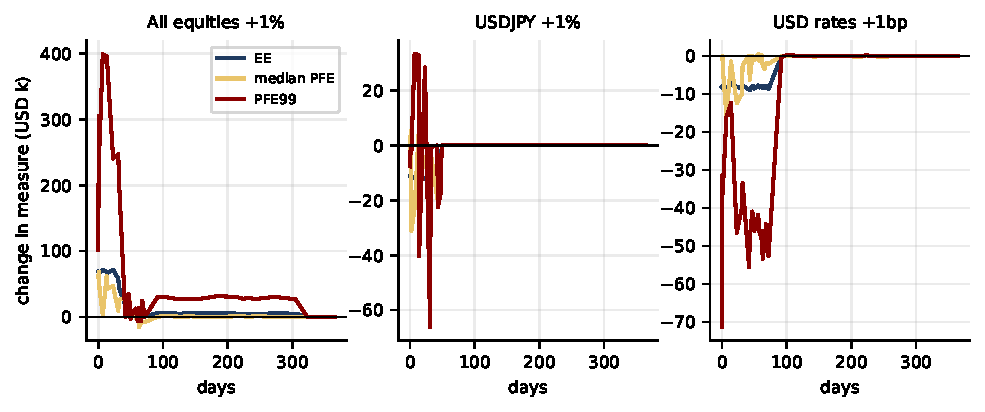
\includegraphics[width=\linewidth]{figures/fig41.pdf}
\caption{Change in portfolio EE, median PFE and PFE99 through time for +1\% on all equities, +1\% on USDJPY and +1bp on USD rates.}
\end{figure}
{\scriptsize\setlength{\LTpre}{4pt}\setlength{\LTpost}{6pt}
\begin{longtable}{>{\raggedright\arraybackslash}p{\dimexpr 0.2568\linewidth-2\tabcolsep\relax}>{\raggedright\arraybackslash}p{\dimexpr 0.1351\linewidth-2\tabcolsep\relax}>{\raggedright\arraybackslash}p{\dimexpr 0.1486\linewidth-2\tabcolsep\relax}>{\raggedright\arraybackslash}p{\dimexpr 0.1486\linewidth-2\tabcolsep\relax}>{\raggedright\arraybackslash}p{\dimexpr 0.1486\linewidth-2\tabcolsep\relax}>{\raggedright\arraybackslash}p{\dimexpr 0.1622\linewidth-2\tabcolsep\relax}}
\toprule
\rowcolor{navy}\textbf{\textcolor{white}{Factor shift}} & \textbf{\textcolor{white}{Measure}} & \textbf{\textcolor{white}{CPTY\_A}} & \textbf{\textcolor{white}{CPTY\_B}} & \textbf{\textcolor{white}{CPTY\_C}} & \textbf{\textcolor{white}{Portfolio}} \\
\endhead
All equities +1\% & EE & 44,381 & 16,333 & 10,834 & 71,548 \\
\rowcolor{gray!9} & Median PFE & 960 & -169 & 2,625 & 46,637 \\
 & PFE99 & 256,223 & 86,182 & 125,847 & 240,468 \\
\rowcolor{gray!9}USDJPY +1\% & EE & 0 & -12,147 & 0 & -12,147 \\
 & Median PFE & 0 & -9,974 & 0 & -4,166 \\
\rowcolor{gray!9} & PFE99 & 0 & -80,451 & 0 & 28,470 \\
USD rates +1bp & EE & -462 & 59 & -7,733 & -8,136 \\
\rowcolor{gray!9} & Median PFE & -980 & 23 & -7,615 & -12,450 \\
 & PFE99 & -405 & 69 & -30,722 & -46,605 \\
\rowcolor{gray!9}Rate volatility +1\% & EE & 313 & 13 & 37,465 & 37,792 \\
 & Median PFE & 1,285 & 259 & 1,133 & 40,219 \\
\rowcolor{gray!9} & PFE99 & -5,330 & 694 & 132,127 & 225,749 \\
FX volatility +1\% & EE & 0 & 0 & 0 & 0 \\
\rowcolor{gray!9} & Median PFE & 0 & 0 & 0 & 0 \\
 & PFE99 & 0 & 0 & 0 & 0 \\
\rowcolor{gray!9}Equity volatility +1\% & EE & 45,999 & 17,068 & 11,321 & 74,389 \\
 & Median PFE & 9,051 & 78 & 1,802 & 75,656 \\
\rowcolor{gray!9} & PFE99 & 241,550 & 69,675 & 100,642 & 251,953 \\
All-equity gamma (+1\%) & EE & 16 & 0 & -0 & 16 \\
\rowcolor{gray!9} & PFE99 & 0 & 0 & -39,253 & 0 \\
USDJPY gamma (+1\%) & EE & 0 & 287 & 0 & 287 \\
\rowcolor{gray!9} & PFE99 & 0 & 1,609 & 0 & -569 \\
Rate gamma (+1bp) & EE & 0 & -0 & 21 & 21 \\
\rowcolor{gray!9} & PFE99 & 0 & -0 & -7,432 & 104 \\
\bottomrule
\end{longtable}}

{\small Change in the measure, in USD, at 2026-09-20. Delta and vega are one-sided shifts read as change per unit shift; gamma is the second difference.}

\textbf{Reading the table.} The equity delta of exposure is negative (EE falls by about \$72k per +1\% on all equities and PFE99 by \$240k): the swaps are pay-equity, so our claim on the counterparty shrinks when shares rise, and the adverse scenarios for credit exposure are equity falls. The USD rate DV01 of PFE99 is positive (\$-47k per +1bp), reflecting the funding legs and bond forwards. The equity and rate gammas of the exposure are positive, as expected for max(V, 0) (a call on the netted value), and small relative to the deltas at a +1\% shift.

\begin{figure}[H]
\centering
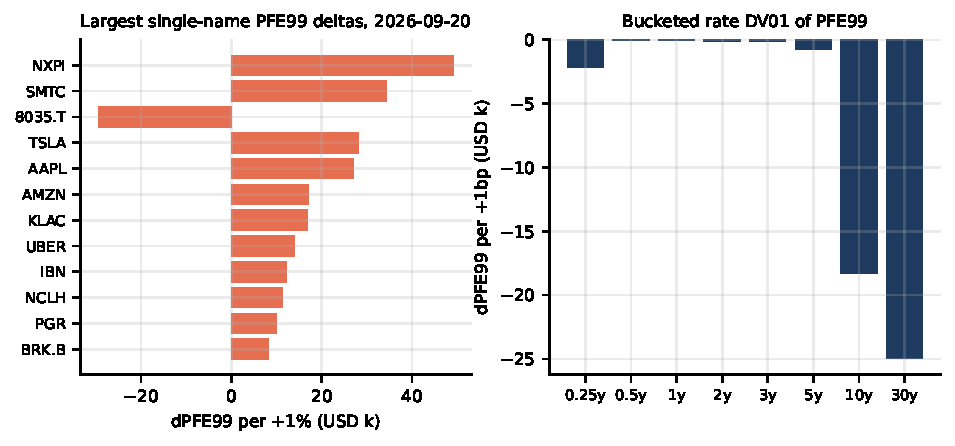
\includegraphics[width=\linewidth]{figures/fig42.pdf}
\caption{Left: the twelve largest single-name deltas of portfolio PFE99 at the peak date. Right: bucketed USD rate DV01 of PFE99 at the same date.}
\end{figure}
Single-name deltas of PFE99 show which positions drive the tail; because a quantile is not additive across names, the single-name deltas sum only approximately to the all-equity delta (Section 9.5).

\subsection{Efficiency}
{\scriptsize\setlength{\LTpre}{4pt}\setlength{\LTpost}{6pt}
\begin{longtable}{>{\raggedright\arraybackslash}p{\dimexpr 0.2857\linewidth-2\tabcolsep\relax}>{\raggedright\arraybackslash}p{\dimexpr 0.1169\linewidth-2\tabcolsep\relax}>{\raggedright\arraybackslash}p{\dimexpr 0.5974\linewidth-2\tabcolsep\relax}}
\toprule
\rowcolor{navy}\textbf{\textcolor{white}{Step (timed at N = 300)}} & \textbf{\textcolor{white}{Cost}} & \textbf{\textcolor{white}{Comment}} \\
\endhead
t = 0 book Greeks & 1.1 s & Central differences on the pricers: every trade, 37 equities, FX, DV01 parallel and 8 buckets \\
\rowcolor{gray!9}Base run (paths and full repricing) & 105 s & 16 trades, all dates, 8 worker processes (includes process start-up) \\
78 equity and FX bumps & 88 s & No re-simulation; only the trades holding the factor are repriced; one process pool. Re-simulating each would cost about 8,521 s (97x more) \\
\rowcolor{gray!9}One rate or volatility re-simulation & 109 s & 13 are needed: parallel up and down, 8 buckets, three vega bumps \\
\bottomrule
\end{longtable}}

The timings in the table were measured on an otherwise idle machine at N = 300, because the production run shared the machine with other jobs; costs scale about linearly with N once process start-up is amortised.

The equity and FX Greeks, which are 37 names plus FX, each with an up and a down bump, cost a small fraction of what naive bump-and-resimulate would. This is the main efficiency gain: it exploits the structure of the model (exact rescaling of GBM paths) rather than approximating anything.

\textbf{What was done, stated plainly.} Every sensitivity is a finite difference of a simulated exposure measure, computed as bump-and-reprice on the same random numbers. For each risk factor: (1) shift the factor (spot by +1\% and -1\%; the curve by +1bp and -1bp in parallel and by bucket; volatilities by +1\% relative); (2) regenerate the paths from the shifted calibration with the same seed and Latin Hypercube draws; (3) reprice the trades on the shifted paths; (4) recompute EE, median PFE and PFE99 by netting set; (5) take the difference from the base run (central difference for delta and gamma, one-sided for vega and bucketed DV01). Because the random numbers are common, the difference is sensitivity and not sampling noise: the standard deviation of the EE delta estimate is \$1k against \$245k with independent draws (282x lower).

\textbf{The efficiency choices.} Two structural facts avoid most of the cost. A spot bump rescales every GBM path exactly, so equity and FX Greeks need no re-simulation; and only the trades holding the bumped factor are repriced (an equity name appears in one to three of the sixteen trades). All 78 equity and FX bumps are priced in one process pool. Curve and volatility bumps change the paths, so they need a re-simulation, but the random numbers are reused and the simulation is a small part of the cost: the repricing of every trade at every node dominates.

{\scriptsize\setlength{\LTpre}{4pt}\setlength{\LTpost}{6pt}
\begin{longtable}{>{\raggedright\arraybackslash}p{\dimexpr 0.3200\linewidth-2\tabcolsep\relax}>{\raggedright\arraybackslash}p{\dimexpr 0.0800\linewidth-2\tabcolsep\relax}>{\raggedright\arraybackslash}p{\dimexpr 0.1200\linewidth-2\tabcolsep\relax}>{\raggedright\arraybackslash}p{\dimexpr 0.1333\linewidth-2\tabcolsep\relax}>{\raggedright\arraybackslash}p{\dimexpr 0.3467\linewidth-2\tabcolsep\relax}}
\toprule
\rowcolor{navy}\textbf{\textcolor{white}{Component}} & \textbf{\textcolor{white}{Count}} & \textbf{\textcolor{white}{Cost each}} & \textbf{\textcolor{white}{Total}} & \textbf{\textcolor{white}{Naive cost (full re-simulation and repricing each time)}} \\
\endhead
Base run (paths and full repricing) & 1 & 105 s & 105 s & - \\
\rowcolor{gray!9}Equity and FX bumps (subset repricing) & 78 & 1.1 s & 88 s & 8,166 s \\
Rate and volatility bumps (re-simulation) & 13 & 109 s & 1,420 s & 1,420 s (same: nothing to save) \\
\rowcolor{gray!9}t = 0 book Greeks (deterministic) & 1 & 1.1 s & 1.1 s & - \\
\bottomrule
\end{longtable}}

Timed at N = 300 on the 8-core development machine, 16 trades, 102 grid nodes, Latin Hypercube; costs scale about linearly in N. The full Greeks set (about 91 factor bumps in total) therefore costs about 1,614 s at N = 300, against about 9,690 s if every equity and FX bump were a re-simulation (6.0x). At the production N = 1,000 the whole set costs roughly 1.5 hours; reporting exposures alone is one base run.

\textbf{Alternatives considered.}

{\scriptsize\setlength{\LTpre}{4pt}\setlength{\LTpost}{6pt}
\begin{longtable}{>{\raggedright\arraybackslash}p{\dimexpr 0.2125\linewidth-2\tabcolsep\relax}>{\raggedright\arraybackslash}p{\dimexpr 0.3250\linewidth-2\tabcolsep\relax}>{\raggedright\arraybackslash}p{\dimexpr 0.4625\linewidth-2\tabcolsep\relax}}
\toprule
\rowcolor{navy}\textbf{\textcolor{white}{Method}} & \textbf{\textcolor{white}{How it works}} & \textbf{\textcolor{white}{Assessment for this book}} \\
\endhead
Bump-and-reprice, independent random numbers & Re-run with a fresh seed for each bump & Unbiased but the noise swamps the difference (282x larger standard deviation here): rejected. \\
\rowcolor{gray!9}Bump-and-reprice, common random numbers (used) & Same draws in base and bumped runs & Works on the pricers as a black box for every measure including quantiles; cost is one repricing per bump, cut by subset repricing. \\
Pathwise (infinitesimal perturbation) & Differentiate the payoff along each path: for a linear-in-spot trade d NPV/d S0 = position x S(t)/S0 & Implemented for equity and FX deltas (greeks/pathwise.py): no repricing at all, exact for EE, noisy for quantiles; validated below. Not applicable to rates without differentiating the pricers. \\
\rowcolor{gray!9}Likelihood ratio & Differentiate the density of the path instead of the payoff & Suits vega-type parameters but has high variance over many time steps: not adopted. \\
Adjoint (algorithmic) differentiation & Backward sweep through pricers and paths gives all Greeks for about 3-5x the cost of one valuation, independent of the number of factors & The asymptotically fastest option (all 37 equity, FX, rate-bucket and vega Greeks in one sweep), but it needs the pricers re-implemented in a differentiable form; the supplied pure-Python pricers are a black box, so it was not possible. It is the recommended route if the pricers are ported. \\
\rowcolor{gray!9}Delta-gamma or regression proxies of the exposure & Fit a cheap approximation of the netted value in the risk factors and differentiate it & Cheap, but the proxy error is added to the Greek and the quantile Greeks are least accurate: reserved for the future, if a Longstaff-Schwartz style proxy is ever built for other purposes. \\
\bottomrule
\end{longtable}}

\textbf{Is there a faster alternative? Yes, for equity and FX.} The pathwise estimator gives every equity and FX delta of every netting set at every reporting date in 0.2 seconds from the paths and NPVs already in memory, against 259 seconds for the 76 bump-and-reprice runs. Compared on the same paths and NPVs, so that both see identical inputs:

{\scriptsize\setlength{\LTpre}{4pt}\setlength{\LTpost}{6pt}
\begin{longtable}{>{\raggedright\arraybackslash}p{\dimexpr 0.2973\linewidth-2\tabcolsep\relax}>{\raggedright\arraybackslash}p{\dimexpr 0.2703\linewidth-2\tabcolsep\relax}>{\raggedright\arraybackslash}p{\dimexpr 0.2162\linewidth-2\tabcolsep\relax}>{\raggedright\arraybackslash}p{\dimexpr 0.2162\linewidth-2\tabcolsep\relax}}
\toprule
\rowcolor{navy}\textbf{\textcolor{white}{Measure}} & \textbf{\textcolor{white}{Names x netting sets compared}} & \textbf{\textcolor{white}{Median max difference}} & \textbf{\textcolor{white}{Worst max difference}} \\
\endhead
EE delta (equity) & 40 & 0.0\% of peak & 0.4\% of peak \\
\rowcolor{gray!9}Median PFE delta (equity) & 40 & 23.0\% of peak & 129.4\% of peak \\
PFE99 delta (equity) & 40 & 7.8\% of peak & 76.0\% of peak \\
\rowcolor{gray!9}EE delta (USDJPY) & 1 & 0.1\% of peak & 0.1\% of peak \\
\bottomrule
\end{longtable}}

{\small Differences are the maximum over reporting dates, as a percentage of the largest single-name delta of the same netting set and measure. The EE deltas agree to numerical precision (the two estimators are algebraically the same up to the kink at zero); the median and PFE99 pathwise deltas are local averages over a few dozen scenarios and are noisier, which is why the bump-and-reprice values remain the reported ones and pathwise is the independent check and the fast path for equity and FX. The remaining cost is the rate and volatility bumps, which no pathwise formula covers here.}

\subsection{Validation of the Greeks}
{\scriptsize\setlength{\LTpre}{4pt}\setlength{\LTpost}{6pt}
\begin{longtable}{>{\raggedright\arraybackslash}p{\dimexpr 0.6053\linewidth-2\tabcolsep\relax}>{\raggedright\arraybackslash}p{\dimexpr 0.3947\linewidth-2\tabcolsep\relax}}
\toprule
\rowcolor{navy}\textbf{\textcolor{white}{Check}} & \textbf{\textcolor{white}{Result}} \\
\endhead
t = 0 equity delta against the analytic value (shares x spot x 1\%, signed by trade direction), all 41 trade-name pairs & maximum relative error 1.6e-02 \\
\rowcolor{gray!9}Bump-size stability of the all-equity EE delta at the peak date: 0.5\%, 1\%, 2\% bumps (USD k per +1\%) & 72, 72, 72 (spread 0.02\%) \\
Additivity: sum of the 37 single-name EE deltas against the all-equity delta (maximum over all dates after t = 0) & 0.06\% of the peak all-equity delta \\
\rowcolor{gray!9}The same at t = 0 itself & 0\%: at t = 0 the exposure max(V, 0) is deterministic and has a kink, and a 1\% bump of one name can cross it (CPTY\_A, CPTY\_B), so single-name and joint finite differences need not add there \\
Sum of single-name PFE99 deltas against the all-equity PFE99 delta at the peak date (quantiles are not additive) & 240 against 240 USD k \\
\rowcolor{gray!9}Common random numbers against independent draws: standard deviation of the EE delta estimate over 3 repeats at N = 300 & 1 USD k against 245 USD k (282x lower) \\
\bottomrule
\end{longtable}}

\begin{figure}[H]
\centering
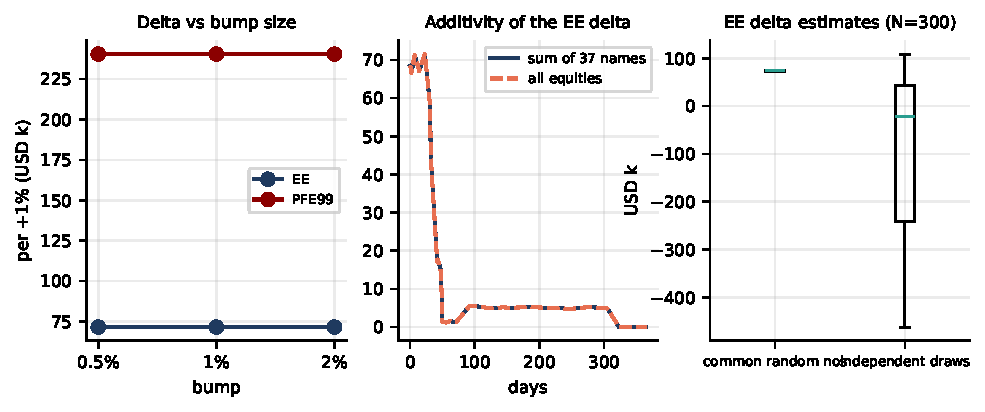
\includegraphics[width=\linewidth]{figures/fig43.pdf}
\caption{Left: delta of EE and PFE99 against bump size. Middle: the sum of the 37 single-name EE deltas equals the all-equity delta through time. Right: estimates of the EE delta with common random numbers and with independent draws.}
\end{figure}
\subsection{Limitations}
\begin{itemize}
\item Sensitivities are finite differences with a 1\% (equity, FX, volatility) or 1bp (rates) shift. The bump-size check above shows the results are stable to a factor of four in bump size.
\item Quantile Greeks (PFE99) carry more estimation noise than EE even with common random numbers; the reported figures use 1,000 scenarios.
\item Interest rate Greeks are for the USD curve only: the simulated JPY rate drives only the drift of JPY-listed names and USDJPY, and no trade is discounted on JPY. There is no inflation, credit-spread or dividend Greek for exposure (credit-spread and vega sensitivities of CVA are in Section 8).
\item Volatility bumps are parallel across each factor class (all equity vols together); there is no vol-surface or per-name vega. No cross-gamma is computed, and theta is represented by the exposure profile itself.
\item Exposure Greeks are for the close-out exposure over the first year at 99\%; the uncollateralized level exposure has much larger sensitivities (its delta is the delta of the mark-to-market itself).
\end{itemize}
\clearpage
\section{Every modelling choice, and what we rejected}
{\scriptsize\setlength{\LTpre}{4pt}\setlength{\LTpost}{6pt}
\begin{longtable}{>{\raggedright\arraybackslash}p{\dimexpr 0.1538\linewidth-2\tabcolsep\relax}>{\raggedright\arraybackslash}p{\dimexpr 0.2564\linewidth-2\tabcolsep\relax}>{\raggedright\arraybackslash}p{\dimexpr 0.2564\linewidth-2\tabcolsep\relax}>{\raggedright\arraybackslash}p{\dimexpr 0.3333\linewidth-2\tabcolsep\relax}}
\toprule
\rowcolor{navy}\textbf{\textcolor{white}{Topic}} & \textbf{\textcolor{white}{Choice}} & \textbf{\textcolor{white}{Alternatives considered}} & \textbf{\textcolor{white}{Reason}} \\
\endhead
Measure & Risk-neutral & Real-world drifts & No unobservable risk premia; verified martingale; horizon short \\
\rowcolor{gray!9}Confidence & PFE99 and median PFE (with EE) & Other percentiles & 99\% is the specified target; 99.9\% needs far more paths for little added insight \\
Exposure & The brief: max(V(t+10bd) - V(t-1bd), 0), signed prior-day variation margin, no initial margin; level exposure as a secondary view & Level max(V,0) only; same-day full-VM MPOR shift & It is what Capitolis specified (kickoff slides 8-9); the level view remains for the uncollateralized case \\
\rowcolor{gray!9}USD rates & Hull-White 1F; sigma fitted to realised 2y-30y Treasury yield vol; Bloomberg long end spliced beyond the futures & CIR, BK, LMM, G2++ (implemented and compared), overnight-SOFR sigma, flat extrapolation & Exact curve fit, analytic bonds, negative-rate capable, few parameters; matches the yield moves the book depends on (Sections 3.2, 11.7) \\
Two-factor rates & G2++ implemented, calibrated to the realised yield covariance; compared, not the default & Two-factor default, swaption-calibrated 2F & Adds a slope factor at 16\% fit error; effect on exposure reported in Section 7.9 \\
\rowcolor{gray!9}Equities/FX & Correlated GBM under the USD measure; quanto correction and rate-driven drifts for JPY names and USDJPY & Heston, SABR, jumps & No option surfaces; matches lognormal vol convention; drifts derived from the martingale condition and tested \\
Volatility & 3y realised & Implied vols & No single-name options data; documented proxy \\
\rowcolor{gray!9}Correlation & One static 40x40 matrix (USD rate on 10-year-yield shocks), Cholesky & Time-varying (DCC), stressed, factor & Data supports one matrix; factor model offered as alternative; correlation stress in Section 7.9 \\
Equity factor model & Optional PCA (k=5) & Full rank only & Robustness, dimension reduction; approximation disclosed \\
\rowcolor{gray!9}Dates & Pillar dates + trade event dates & Monthly grid & Industry convention, denser where risk moves, exact cash-flow dates \\
Sampling & Latin Hypercube & Pseudo-random, antithetic, moment-matched, Sobol & Best measured error on both test and real engine \\
\rowcolor{gray!9}Scenario count & 5,000 (reporting); 1,000 (iteration); 10,000 (sign-off) & 30,000 pool & Diminishing returns beyond 10-15k; model risk dominates \\
Mean reversion a & Swaption-based (USD 0.0167) & Futures proxy (0.0458), textbook 0.03 & Industry-standard instrument \\
\rowcolor{gray!9}JPY rates & Real JPY Hull-White factor, simulated and correlated with the USD rate, USDJPY and the equities & Constant differential only & Negative-rate capable; sigma from the real JPY OIS history; correlations calibrated \\
Collateral & Close-out exposure with daily VM at the prior-day value; uncollateralized level exposure alongside & Assume full VM with same-day margin & No CSA data: the two definitions bracket the answer \\
\rowcolor{gray!9}xVA and capital & CVA on both exposure definitions; DVA and FVA on assumed own credit and funding spreads; SA-CVA; SA-CCR EAD & CVA only; BA-CVA & Extra-credit scope; assumptions stated and sensitivities shown \\
Greeks & Bump-and-reprice with common random numbers; subset repricing for equity and FX; pathwise for equity and FX as a fast check & Independent draws, likelihood ratio, adjoint (needs pricer port) & Works on the black-box pricers; cost measured (Section 9.4) \\
\rowcolor{gray!9}Model validation & Martingale tests, VaR benchmark, Kupiec backtest, attribution, model-risk study, stress test & Narrative stress test & Quantified, out-of-sample where possible (Sections 7.3, 7.9, 7.10, 11) \\
Pricing & Reuse validated pricer library & Vectorised reimplementation & Correctness first; speed via multiprocessing \\
\bottomrule
\end{longtable}}

\clearpage
\section{Validation: how we know the engine is right}
Each check isolates one layer (paths, pricing, calibration, aggregation) so a failure points at where to look.

\subsection{Self-consistency at t = 0}
Simulated EE(0) must equal a direct current-exposure calculation from the identical calibrated snapshot: matches to 0.0000\% (after fixing two comparison-object mismatches, Section 10).

\subsection{Martingale / no-arbitrage test}
Under the risk-neutral measure discounted asset prices must have no drift. With 8,000 paths: the bank-account check E[exp(-integral r)] = P(0,T) holds to a maximum relative difference of 0.85 bp across nodes (a small, understood trapezoid-integration effect of the time grid); the discounted `gains process' of 6 names (four USD-listed and two JPY-listed, the latter valued in USD as S / X) has all \textbar{}z\textbar{} below 1.5; and the JPY bank account valued in USD, B\_JPY / (X B\_USD), is a martingale with z = +0.03, while ln USDJPY drifts by -0.0287 over the horizon (down, as it must when USD rates exceed JPY rates). This validates the drift terms in the engine itself, including the quanto correction and the JPY-rate drift, independent of any trade pricing. The earlier version of this test covered only the six highest-volatility names and so did not exercise the JPY drift; the USDJPY drift sign error found later (Section 12) was outside its reach.

\subsection{Parametric (delta-normal) VaR benchmark}
An independent standard method: portfolio dollar-deltas by bump-and-reprice with the same volatilities and correlations as the simulation, combined into a delta-normal VaR at the first simulated node (one day, the overnight pillar). The 99\% delta-normal VaR is \$12.6M against \$12.1M from the Monte Carlo P\&L distribution (ratio 1.04; accepted range 0.3-1.3). At this short horizon the book is close to linear in the risk factors, so close agreement is expected; a large discrepancy would have indicated a sign or scaling error in the deltas or the covariance.

\subsection{Stress and sensitivity tests}
The earlier directional test (a few bumps of volatility and the curve, one paragraph of results) has been replaced by the structured programme of Sections 7.9 (one-at-a-time model perturbations) and 7.10 (stress scenarios with stated data and inputs, by netting set, by trade and along the time path), which answers what the inputs were, how sensitive the outputs are across the path, and whether all products react.

\subsection{Statistical and unit tests}
142 automated tests pass. They cover: Hull-White reproducing the curve at t=0 to 1e-9; the GBM martingale property; the 1/sqrt(N) error law; antithetic variance reduction; Cholesky recovering a target correlation; MPOR look-ahead spacing and formula; pillar dates and forced event dates; negative-rate behaviour of Hull-White; the PCA factor model (exact at full rank, monotone error, variance preservation); the BOJ TONA and MOF JGB loaders and the empirical JPY findings; the tail-convergence result; median PFE, CVA and the SA-CVA aggregation, the credit-spread proxy curves, and the Greeks machinery (bump helpers, t=0 Greeks against analytic values, exposure measures); and, added in this version, the close-out exposure convention (signed variation margin, netting before the positive part, settlement inside the window, the t-1bd node), the Bloomberg long-end splice, the JPY factor (curve fit, shock correlations, and the USDJPY and JPY-name martingale properties including a regression test for the drift sign), the long-end volatility fit, the G2++ model (curve fit, martingale property, calibration recovery, engine integration), DVA and FVA against closed forms, SA-CCR against hand calculations, the Kupiec and Christoffersen tests and both backtests, the stress-scenario helpers, the pathwise Greeks against central bumps, and the risky-bond sample.

\subsection{Greeks (sensitivities)}
Three delta estimators were compared on a call option: pathwise, bump-and-reprice with \textbf{common random numbers} (same draws in base and bumped runs) and bump-and-reprice with independent draws.

{\footnotesize\setlength{\LTpre}{4pt}\setlength{\LTpost}{6pt}
\begin{longtable}{>{\raggedright\arraybackslash}p{\dimexpr 0.3824\linewidth-2\tabcolsep\relax}>{\raggedright\arraybackslash}p{\dimexpr 0.1912\linewidth-2\tabcolsep\relax}>{\raggedright\arraybackslash}p{\dimexpr 0.2353\linewidth-2\tabcolsep\relax}>{\raggedright\arraybackslash}p{\dimexpr 0.1912\linewidth-2\tabcolsep\relax}}
\toprule
\rowcolor{navy}\textbf{\textcolor{white}{Method}} & \textbf{\textcolor{white}{Bias}} & \textbf{\textcolor{white}{Std of estimate}} & \textbf{\textcolor{white}{Time/trial}} \\
\endhead
Pathwise & +0.000085 & 0.003771 & 0.470 ms \\
\rowcolor{gray!9}Bump, common random numbers & +0.000033 & 0.003742 & 0.327 ms \\
Bump, independent random numbers & -0.003502 & 0.096885 & 0.850 ms \\
\bottomrule
\end{longtable}}

Common random numbers make bump-and-reprice statistically indistinguishable from the pathwise estimator (26x lower noise than independent draws), and it works on any pricer as a black box, so it is the method that generalises to the real book. On the real book, the exact t=0 delta of EQTRS\_0003's NPV to its largest position is -\$212,269 per \$1 move, exactly equal to the share count (a linear-payoff consistency check).

On the real book the pathwise estimator was also validated against the bump-and-reprice deltas of the close-out exposure (Section 9.4).

\subsection{Backtesting: Kupiec proportion-of-failures tests}
A model that is correct on average can still misstate the tail. The simulated exposure quantiles were therefore backtested against realised history, with the Kupiec proportion-of-failures test (Basel's standard backtest). At each historical as-of date the model is calibrated using only data up to that date (a trailing 3-year window), asked for the 95th and 99th percentile of the 10-business-day change in value of a fixed set of positions, and the realised change is read off history. An exception is a realised move above the predicted quantile; a correct model has exceptions with probability 5\% or 1\%, independently. Windows do not overlap, and the starting phase is shifted over ten offsets to check robustness. The equity leg uses the actual equity TRS positions of each counterparty (JPY names through USDJPY) and the engine's own lognormal model on 2014-06-02 to 2026-08-28 daily data; the rates leg tests the Hull-White distribution of 10-day yield changes at 5, 10 and 20 years.

\textbf{Equity and FX leg} (upper-tail exceptions; the exposure is the gain side of the position):

{\scriptsize\setlength{\LTpre}{4pt}\setlength{\LTpost}{6pt}
\begin{longtable}{>{\raggedright\arraybackslash}p{\dimexpr 0.1169\linewidth-2\tabcolsep\relax}>{\raggedright\arraybackslash}p{\dimexpr 0.0779\linewidth-2\tabcolsep\relax}>{\raggedright\arraybackslash}p{\dimexpr 0.1299\linewidth-2\tabcolsep\relax}>{\raggedright\arraybackslash}p{\dimexpr 0.1039\linewidth-2\tabcolsep\relax}>{\raggedright\arraybackslash}p{\dimexpr 0.0909\linewidth-2\tabcolsep\relax}>{\raggedright\arraybackslash}p{\dimexpr 0.1299\linewidth-2\tabcolsep\relax}>{\raggedright\arraybackslash}p{\dimexpr 0.1818\linewidth-2\tabcolsep\relax}>{\raggedright\arraybackslash}p{\dimexpr 0.1688\linewidth-2\tabcolsep\relax}}
\toprule
\rowcolor{navy}\textbf{\textcolor{white}{Netting set}} & \textbf{\textcolor{white}{Level}} & \textbf{\textcolor{white}{Exceptions}} & \textbf{\textcolor{white}{Expected}} & \textbf{\textcolor{white}{Rate}} & \textbf{\textcolor{white}{Kupiec p-value}} & \textbf{\textcolor{white}{Offsets rejecting (of 10)}} & \textbf{\textcolor{white}{Mean rate over offsets}} \\
\endhead
CPTY\_A & 95\% & 8 of 242 & 12.1 & 3.3\% & 0.20 & 5 & 3.0\% \\
\rowcolor{gray!9}CPTY\_A & 99\% & 4 of 242 & 2.4 & 1.7\% & 0.35 & 0 & 1.4\% \\
CPTY\_B & 95\% & 11 of 242 & 12.1 & 4.5\% & 0.74 & 0 & 5.3\% \\
\rowcolor{gray!9}CPTY\_B & 99\% & 6 of 242 & 2.4 & 2.5\% & 0.05 & 4 & 2.6\% \\
CPTY\_C & 95\% & 7 of 242 & 12.1 & 2.9\% & 0.10 & 3 & 3.2\% \\
\rowcolor{gray!9}CPTY\_C & 99\% & 2 of 242 & 2.4 & 0.8\% & 0.78 & 0 & 1.2\% \\
\bottomrule
\end{longtable}}

\begin{figure}[H]
\centering
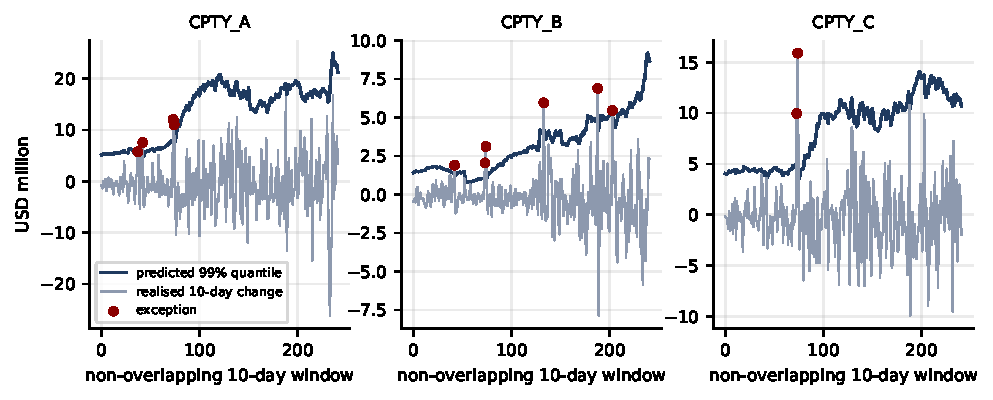
\includegraphics[width=\linewidth]{figures/fig44.pdf}
\caption{Predicted 99\% quantile of the 10-day change in each netting set's equity positions against the realised change, over the whole backtest; exceptions in red.}
\end{figure}
\textbf{Rates leg} (10-day change of the Treasury CMT yield against the one-factor Hull-White distribution, as-of dates from 2020-04-03):

{\scriptsize\setlength{\LTpre}{4pt}\setlength{\LTpost}{6pt}
\begin{longtable}{>{\raggedright\arraybackslash}p{\dimexpr 0.0822\linewidth-2\tabcolsep\relax}>{\raggedright\arraybackslash}p{\dimexpr 0.2055\linewidth-2\tabcolsep\relax}>{\raggedright\arraybackslash}p{\dimexpr 0.1781\linewidth-2\tabcolsep\relax}>{\raggedright\arraybackslash}p{\dimexpr 0.1781\linewidth-2\tabcolsep\relax}>{\raggedright\arraybackslash}p{\dimexpr 0.1781\linewidth-2\tabcolsep\relax}>{\raggedright\arraybackslash}p{\dimexpr 0.1781\linewidth-2\tabcolsep\relax}}
\toprule
\rowcolor{navy}\textbf{\textcolor{white}{Tenor}} & \textbf{\textcolor{white}{Sigma from}} & \textbf{\textcolor{white}{99\% up: exceptions}} & \textbf{\textcolor{white}{99\% up: mean rate}} & \textbf{\textcolor{white}{95\% up: mean rate}} & \textbf{\textcolor{white}{95\% down: mean rate}} \\
\endhead
5y & overnight SOFR vol & 1 of 161 & 1.0\% & 3.7\% & 2.8\% \\
\rowcolor{gray!9}5y & long-end fit & 4 of 161 & 1.9\% & 5.7\% & 3.0\% \\
10y & overnight SOFR vol & 1 of 161 & 0.4\% & 3.1\% & 2.2\% \\
\rowcolor{gray!9}10y & long-end fit & 3 of 161 & 1.4\% & 5.6\% & 2.7\% \\
20y & overnight SOFR vol & 1 of 161 & 0.6\% & 3.3\% & 2.2\% \\
\rowcolor{gray!9}20y & long-end fit & 3 of 161 & 1.4\% & 5.8\% & 2.5\% \\
\bottomrule
\end{longtable}}

{\small Nominal exception rates are 1\% at the 99\% level and 5\% at the 95\% level.}

\textbf{What the backtest shows.} At the 99\% level the equity and FX quantiles are close to calibrated: the exceptions are 4/6/2 against 2.4/2.4/2.4 expected, and the Kupiec test does not reject for 3 of the three netting sets at the 5\% level on the base offset (CPTY\_B, with 6 exceptions against 2.4, is the borderline case, consistent with the fat tails that geometric Brownian motion understates). At the 95\% level the model is conservative for CPTY\_A and CPTY\_C (mean exception rates 3.0\% and 3.2\% against 5\%): a Kupiec test is two-sided, so being too conservative can also fail it (5 of the 10 offsets reject for CPTY\_A at this level). With about 242 non-overlapping windows per series the test has limited power, which is why the counts, not only the p-values, are shown. On the rates leg both calibrations of sigma pass on average over 2020-2026, but they are not equivalent: the long-end fit gives mean exception rates of 5.7\% at the 95\% up-tail and 1.5\% at the 99\% up-tail (nominal 5\% and 1\%), while the overnight-SOFR calibration gives 3.4\% and 0.7\%, i.e. it was too wide on average, reflecting a calibration window that included the 2022-23 hiking cycle, and would be too narrow in a period such as the present, when SOFR is stable and long yields are not (its current value is 63bp against 96bp for the fit). The long-end fit is therefore the more stable calibration.

\clearpage
\section{Defects identified and resolved}
Each defect was identified by checking against an independent source, a hand calculation or a full end-to-end run.

{\scriptsize\setlength{\LTpre}{4pt}\setlength{\LTpost}{6pt}
\begin{longtable}{>{\raggedright\arraybackslash}p{\dimexpr 0.0385\linewidth-2\tabcolsep\relax}>{\raggedright\arraybackslash}p{\dimexpr 0.4231\linewidth-2\tabcolsep\relax}>{\raggedright\arraybackslash}p{\dimexpr 0.5385\linewidth-2\tabcolsep\relax}}
\toprule
\rowcolor{navy}\textbf{\textcolor{white}{\#}} & \textbf{\textcolor{white}{Bug}} & \textbf{\textcolor{white}{How it was caught / fix}} \\
\endhead
1 & BRK.B vs BRK-B ticker silently failed in two functions & Missing prices; fixed in both current and historical fetch \\
\rowcolor{gray!9}2 & SOFR curve: recently-expired serial futures wrapped a decade forward, creating a multi-year gap & Cross-check against Treasury.gov par curve (73bp vs smooth 56bp at 10Y); fixed \\
3 & The fix for \#2 over-corrected and dropped genuine far-dated live contracts (e.g. SR3H0, March 2030) & Found while calibrating Hull-White; fixed with a 400-day plausibility threshold; curve coverage 3.6y -\textgreater{} 6.3y \\
\rowcolor{gray!9}4 & US and Tokyo equity histories joined by timestamp gave a $\sim$70\% blank table & Join by calendar date instead \\
5 & Stale cached exposure file gave false 7-15\% `discrepancies' & Root cause: real overnight moves (one name has 76\% vol); check now uses the in-memory snapshot \\
\rowcolor{gray!9}6 & Residual 0.02-0.03\% self-check gap & Different curve object; both sides now use the identical exact analytic curve: 0.0000\% \\
7 & Tail-convergence study initially run at 99.9\% rather than the specified 99\% & Re-run at 99\%; tests and documentation updated \\
\rowcolor{gray!9}8 & JPY mean-reversion fit gave a negative a & Diagnosed as a real structural property (three sources); lower bound a = 0.001 used \\
9 & Headline exposure was the uncollateralized level max(V, 0), not the brief's move from the prior-day NPV over a 10-day close-out & Found by reviewing the work against the kickoff deck and an independent implementation of the same brief; exposure module, t-1bd grid node and tests added (Section 7.1) \\
\rowcolor{gray!9}10 & USD curve extrapolated flat beyond the last futures contract (about 6.5 years), understating the long-dated Treasury forward BF\_0003 by about 16\% & Found by repricing BF\_0003 on Bloomberg's own zero curve; long end spliced (Section 3.1); NPV reconciled to within 0.4\% \\
11 & USDJPY drift had the wrong sign (the drift of USD per JPY used for JPY per USD), so JPY-listed names drifted about 2 x 2.6\% a year too low in USD value & Found while deriving the drifts for the JPY factor from the martingale condition; the old martingale test only covered six high-volatility names. Drifts corrected, quanto term added, martingale tests for JPY names and the JPY bank account added (Section 4.2) \\
\rowcolor{gray!9}12 & USD Hull-White sigma taken from the overnight SOFR fixing understated the moves of the 2y-30y yields (10-day 20y-yield move: about 15bp realised against 11bp modelled) & Found by comparing modelled and realised 10-day yield moves and confirmed by the rates backtest; sigma fitted to realised long-end volatility (Section 3.2) \\
13 & Equity histories on different exchange holidays left gaps that emptied the first backtest windows & Last close carried over non-trading days (at most five) before returns are taken \\
\bottomrule
\end{longtable}}

\section{Assumptions and limitations}
\begin{itemize}
\item \textbf{No CSA data.} The exposure headline assumes daily variation margin at the prior-day value and no initial margin, as the brief specifies; the uncollateralized level view brackets the other extreme. Threshold, minimum transfer amount and initial margin are unknown (Section 7.7 shows the size of the effect of margin).
\item \textbf{Volatility is a 3-year realised proxy}, not implied. Regime shifts and skew are not captured; volatility is stressed in Sections 7.9 and 7.10.
\item \textbf{One static correlation matrix} from 616 days; correlations tend to rise in stress and are stressed only in the model-risk study (Section 7.9).
\item \textbf{GBM underestimates fat tails}, most relevant for PFE99 on high-vol names; the backtest shows it (CPTY\_B at 99\%).
\item \textbf{Rates:} the base model has a single USD factor (no curve twist independent of the level); a two-factor G2++ is implemented and its effect measured, but it fits the realised covariance with a 16\% error and is not the default. The JPY rate has mean reversion at its lower bound because every calibration gives a negative value.
\item \textbf{Risk-neutral drift}: not a real-world forecast; regulatory PFE may need physical drift. The backtest compares model quantiles with realised moves and is the check on this.
\item \textbf{Model risk vs sampling risk:} above a few thousand scenarios the uncertainty is in the models, not the random numbers (Section 7.9).
\item \textbf{Own credit and funding} for DVA and FVA are assumptions (BBB proxy, funding spread equal to the own spread). \textbf{SA-CCR} is unmargined, single-name equity and USD interest-rate only, with no collateral. \textbf{Risky bonds} use a bond-index proxy for the issuer curve with deterministic spreads.
\item \textbf{Stress tests} are instantaneous shocks to the starting state with the base model's volatilities, correlations and mean reversion; they are not a projection, and the historical replays cover 2014-2026 only (no 2008).
\item \textbf{Backtests} have limited power at 99\% (a few exceptions in about 240 windows) and test static positions, not the evolving book; the rates leg tests yield moves, not the book's rate exposure directly.
\item \textbf{No wrong-way risk or credit dynamics of the counterparty itself}; this is exposure, not a loss estimate (that needs PD and LGD).
\item \textbf{Bloomberg data is a single 2026-08-31 snapshot} (three days after the 2026-08-28 market data), re-based to our reference date; acceptable for shape and level, disclosed.
\end{itemize}
\section{Conclusions and recommendations}
\begin{itemize}
\item The engine is validated (t=0 self-check, martingale tests including the JPY components, delta-normal VaR benchmark, Kupiec backtest, 142 automated tests) and reproducible with a single command per stage.
\item On the exposure definition in the brief (10-day close-out from the prior-day value), the portfolio MPE99 is \$51.0M at 2026-09-20, with peak EE of \$11.6M and peak median PFE of \$8.2M (Section 7.1). The earlier version of this work reported \$45.7M before the model corrections of Section 7.3.
\item The portfolio MPE99 is 78\% of the sum of the counterparty MPE99s: netting does not cross counterparties and the three books peak within about four weeks of each other, so there is little diversification (Section 7.2).
\item The uncollateralized level exposure, kept as a secondary view, has peak portfolio PFE99 of \$201.9M at 2026-10-09, versus EE of \$140.1M and median PFE of \$140.3M; the spread between these three is the point of reporting all of them.
\item Risk is short-dated (about four months) and concentrated: CPTY\_C, through the single 500M bond forward, dominates the level exposure and the current exposure. On the close-out definition CPTY\_C (the 10-day rate move of that forward) and the equity netting set CPTY\_A are the two largest, with CPTY\_B small.
\item CVA is about \$12k on the close-out exposure and \$247k on the uncollateralized level exposure at a BBB proxy; DVA is \$11k and FVA \$1k on assumed own credit and funding spreads; the SA-CVA requirement is \$0.10M on the close-out exposure and \$2.23M (RWA \$27.8M) on the uncollateralized exposure, and the SA-CCR exposure at default \$260.3M.
\item Greeks are complete for the book and for the exposure measures (Section 9). Their cost is dominated by the rate and volatility re-simulations; equity and FX Greeks cost a small fraction of naive bumping through subset repricing, and pathwise estimators give them in seconds. PFE99 at its peak date falls by about \$240k per +1\% on all equities and moves by about \$47k per +1bp on USD rates.
\item Stress: the largest portfolio move of the close-out MPE99 is -24\% (Stagflation) against +86\% (Stagflation) for the level exposure: the margined measure is much less sensitive to level shocks than the uncollateralized one, and sensitivity is product specific (Section 7.10).
\item Backtest: the 99\% quantiles of the equity and FX leg are close to calibrated (CPTY\_B slightly light-tailed), and the long-end yield-vol calibration is more stable than the overnight-SOFR one (Section 11.7).
\item We recommend confirming with Capitolis whether any trade is margined, and on what terms; that fact matters more than any further modelling refinement.
\item Use Latin Hypercube sampling with N = 5,000 for reporting, N = 1,000 for iteration and N = 10,000 for limit sign-off (Section 5.5).
\item What remains is data and scope, not engineering: real counterparty ratings or CDS, CSA terms, wrong-way risk, and the items in Section 15.
\end{itemize}
\clearpage
\section{Remaining work and open questions}
Everything in the plan that could be completed with the data and information available has been done and is reported above. What remains depends on information Capitolis holds, or is a longer-term refinement. It is listed here with what is needed, so the next session can decide which to take forward.

{\scriptsize\setlength{\LTpre}{4pt}\setlength{\LTpost}{6pt}
\begin{longtable}{>{\raggedright\arraybackslash}p{\dimexpr 0.3077\linewidth-2\tabcolsep\relax}>{\raggedright\arraybackslash}p{\dimexpr 0.4615\linewidth-2\tabcolsep\relax}>{\raggedright\arraybackslash}p{\dimexpr 0.2308\linewidth-2\tabcolsep\relax}}
\toprule
\rowcolor{navy}\textbf{\textcolor{white}{Item}} & \textbf{\textcolor{white}{Why it is open}} & \textbf{\textcolor{white}{What is needed}} \\
\endhead
Real counterparty ratings or CDS for CPTY\_A, CPTY\_B, CPTY\_C & The counterparties are anonymised and no CDS quotes could be sourced; the BBB proxy drives every credit number (Section 8.3 shows the range) & Names or ratings, or CDS quotes \\
\rowcolor{gray!9}Credit support annexes (threshold, minimum transfer amount, initial margin) & Not in the data; the two exposure definitions of Section 7 bracket the answer & Terms per netting set \\
Wrong-way risk in CVA & Independence of exposure and default is assumed & A decision on the dependence model and on which counterparties it applies to \\
\rowcolor{gray!9}Risky bonds and CDS beyond the proxy & The sample of Section 8.9 uses a bond-index issuer curve with deterministic spreads; no CDS pricer exists in the library and no CDS data was obtainable & CDS quotes; a CDS pricer; stochastic issuer spreads \\
All-factor Greeks by adjoint differentiation & The cheapest route for rate and volatility Greeks, but the supplied pricers are a black box (Section 9.4) & A differentiable port of the pricers \\
\rowcolor{gray!9}Two-factor model as the default & G2++ is implemented and compared (Sections 4.6, 7.9); its calibration is to realised yield covariance with a 16\% fit error & Calibration to the swaption cube and a decision on adoption \\
Hybrid sampling for the PCA factor model & Section 4.4 shows the factor model adds no speed and no accuracy as implemented & Draw the systematic factors quasi-randomly and the idiosyncratic noise pseudo-randomly, then re-measure \\
\rowcolor{gray!9}Stochastic volatility and skew & Needs single-name option surfaces, which the data does not include & Option data, or an index-basis assumption \\
Production hardening & Vectorised pricers if scenario counts must exceed about 10,000; scheduling, monitoring and independent validation by Capitolis Risk & Scope and infrastructure decisions \\
\bottomrule
\end{longtable}}

The CVA questions to settle at the next session are listed at the end of Section 8.7.

\clearpage
\clearpage
\appendix
\section{Glossary}
{\footnotesize\setlength{\LTpre}{4pt}\setlength{\LTpost}{6pt}
\begin{longtable}{>{\raggedright\arraybackslash}p{\dimexpr 0.2857\linewidth-2\tabcolsep\relax}>{\raggedright\arraybackslash}p{\dimexpr 0.7143\linewidth-2\tabcolsep\relax}}
\toprule
\rowcolor{navy}\textbf{\textcolor{white}{Term}} & \textbf{\textcolor{white}{Meaning}} \\
\endhead
Counterparty credit risk (CCR) & Loss risk if the other side of a derivative defaults while the contract is in our favour \\
\rowcolor{gray!9}MTM / NPV & Mark-to-market / net present value: what the trade is worth today \\
Netting set & Trades under one legal netting agreement; combined before taking max(V,0) \\
\rowcolor{gray!9}EE, PFE, MPE & Expected exposure (mean), potential future exposure (percentile), maximum PFE over time \\
Median PFE & 50th percentile of exposure at a date \\
\rowcolor{gray!9}Total return swap (TRS) & Swap exchanging an asset's total return for a funding rate \\
Compo & Payoff in one currency on an asset quoted in another, so both asset and FX move the value \\
\rowcolor{gray!9}SOFR / OIS & US overnight risk-free rate / overnight index swap; the discount curve \\
TONA & Tokyo Overnight Average rate, JPY's overnight risk-free rate \\
\rowcolor{gray!9}Hull-White & Gaussian mean-reverting short-rate model that fits today's curve exactly \\
Mean reversion (a) & Speed at which a rate is pulled back toward its long-run path \\
\rowcolor{gray!9}GBM & Geometric Brownian motion: lognormal price dynamics \\
Cholesky & Factorisation C = L L' used to create correlated random draws \\
\rowcolor{gray!9}PCA / factor model & Explain most co-movement with a few principal factors plus idiosyncratic noise \\
Latin Hypercube / Sobol & Stratified / low-discrepancy sampling schemes that reduce Monte Carlo noise \\
\rowcolor{gray!9}Common random numbers & Reuse identical random draws across compared runs so differences are not noise \\
MPOR & Margin period of risk: delay between last margin call and close-out (typically 10 business days) \\
\rowcolor{gray!9}CSA / VM / threshold & Credit support annex / variation margin / uncollateralized amount before margin is called \\
Delta, gamma & First and second sensitivity of a value or exposure measure to a market factor (here per +1\% spot, per +1bp rate) \\
\rowcolor{gray!9}DV01 & Change in value for a +1bp move of the interest rate curve, parallel or by tenor bucket \\
Vega & Sensitivity to volatility (here per +1\% relative shift) \\
\rowcolor{gray!9}CVA & Credit valuation adjustment: the market price of counterparty default risk on a derivatives portfolio \\
SA-CVA & Basel standardised approach for CVA capital: risk-weighted CVA sensitivities aggregated by bucket and risk class (MAR50) \\
\rowcolor{gray!9}Wrong-way risk & Positive dependence between exposure and the counterparty default probability (not modelled here) \\
SIMM & ISDA Standard Initial Margin Model: sensitivity-based initial margin for uncleared derivatives, calibrated to a 99\% 10-day loss (not implemented here) \\
\rowcolor{gray!9}Pillar dates & Standard curve tenor points: O/N, T/N, 1W, 2W, 1M ... 10Y \\
Close-out exposure & max(V(t + 10bd) - V(t - 1bd), 0): the move of the netted value over a 10-business-day close-out from the prior-day value, which is the variation margin; the brief's definition \\
\rowcolor{gray!9}DVA, FVA & Debit valuation adjustment (own default, on the negative exposure); funding valuation adjustment (cost of funding the exposure less the benefit) \\
SA-CCR, EAD & Basel standardised approach for counterparty credit risk; exposure at default = 1.4 x (replacement cost + multiplier x add-on) \\
\rowcolor{gray!9}G2++ & Two-factor Gaussian short-rate model (equivalent to a two-factor LGM) with a level and a slope factor \\
Kupiec test & Likelihood-ratio test of whether the observed frequency of exceptions matches the nominal probability \\
\rowcolor{gray!9}Pathwise delta & Sensitivity obtained by differentiating the payoff along each simulated path instead of bumping and repricing \\
Stress scenario & An instantaneous shock to today's market state, followed by the full exposure simulation from that state \\
\rowcolor{gray!9}Risk-neutral measure & Pricing measure in which discounted assets are martingales; drift = r - q \\
\bottomrule
\end{longtable}}

\section{Data sources and lineage}
Every external input, where it came from, how it was obtained and what it is used for. Raw pulls are stored under data/raw/ (excluded from version control); licensed data is never redistributed.

{\scriptsize\setlength{\LTpre}{4pt}\setlength{\LTpost}{6pt}
\begin{longtable}{>{\raggedright\arraybackslash}p{\dimexpr 0.1954\linewidth-2\tabcolsep\relax}>{\raggedright\arraybackslash}p{\dimexpr 0.2299\linewidth-2\tabcolsep\relax}>{\raggedright\arraybackslash}p{\dimexpr 0.1839\linewidth-2\tabcolsep\relax}>{\raggedright\arraybackslash}p{\dimexpr 0.2529\linewidth-2\tabcolsep\relax}>{\raggedright\arraybackslash}p{\dimexpr 0.1379\linewidth-2\tabcolsep\relax}}
\toprule
\rowcolor{navy}\textbf{\textcolor{white}{Input}} & \textbf{\textcolor{white}{Source}} & \textbf{\textcolor{white}{How obtained}} & \textbf{\textcolor{white}{Used for}} & \textbf{\textcolor{white}{Status}} \\
\endhead
Trades (16) and underlyings & Capitolis: trade\_data/*.csv & Supplied files & Trade definitions, baskets, bonds & Given \\
\rowcolor{gray!9}Pricing library & Capitolis: capitolis\_pricers & Supplied package (standard library only) & All trade valuation (npv), curves, day counts & Given; independently reviewed \\
USD SOFR futures (SR3, SR1) & CME Globex via Databento (dataset GLBX.MDP3) & Paid API; key only in an environment variable & USD discount curve (bootstrapped by us), Hull-White fit, futures-vol mean-reversion cross-check & Live, validated against Treasury.gov \\
\rowcolor{gray!9}Treasury par yield curve & U.S. Treasury (treasury.gov) & Public download & Independent check of the SOFR curve & Validation only \\
Equity spots, dividends, 3y price history (37 names) & yfinance (Yahoo Finance) & Public API, keyed by ISIN & GBM start values and drift, realised volatility, correlation & Live \\
\rowcolor{gray!9}USDJPY spot and 3y history & yfinance & Public API & FX start value, volatility, correlation & Live \\
SOFR level history & FRED (series SOFR) & Public CSV & Rate volatility; USD-JPY rate correlation & From April 2018 \\
\rowcolor{gray!9}TONA (JPY overnight rate), 1998 to date & Bank of Japan Time-Series Data Search API (DB FM01, series STRDCLUCON) & Public API & JPY rate volatility; USD-JPY correlation; negative-rate evidence & Public \\
JGB par yields 1Y-40Y, 1974 to date & Japan Ministry of Finance & Public CSV (browser-like request headers) & Test of JPY mean reversion & Public \\
\rowcolor{gray!9}JPY OIS par-rate history (MUTKCALM overnight plus 35 OIS tenors, 5 Oct 2011 to 18 Sep 2026) & Bloomberg (tickers JYSO*, MUTKCALM Index) & Provided by the project team, saved as data/raw/sources/JPY.xlsx (parsed copy jpy\_ois\_history.csv) & JPY zero curve (bootstrapped), JPY volatility, JPY-USD differential, mean-reversion test & Licensed: derived numbers only in the report \\
USD and JPY swaption cubes; USDJPY forward points & Bloomberg one-time export, snapshot 2026-08-31 & Provided by the project team & USD mean reversion; JPY cross-check; FX forwards & Licensed: derived numbers only in the report \\
\rowcolor{gray!9}Credit spreads by rating and maturity shape & FRED: ICE BofA US option-adjusted spread indices & Public CSV & Counterparty credit spread proxy for CVA & Public \\
SA-CVA parameters and formulas & BIS, Basel Framework MAR50 (July 2020 revisions) & Public PDF & Risk weights, correlations, aggregation & Public \\
\rowcolor{gray!9}Equity sector, country, market cap & yfinance & Public API & SA-CVA equity buckets & Live \\
Treasury constant-maturity yields 3M-30Y & FRED (DGS3MO ... DGS30) & Public CSV & USD rate sigma, correlations, G2++, backtest, stress replays & Public \\
\rowcolor{gray!9}Long price history 2014-2026 (37 names) and USDJPY & yfinance & Public API, cached in data/raw & Backtest and historical stress windows & Public \\
USD SOFR zero curve, long end & Bloomberg one-time export, 2026-08-31 & Provided by the project team & Spliced onto the futures curve beyond the last contract & Licensed: derived numbers only \\
\bottomrule
\end{longtable}}

Assumptions that are not sourced from data: counterparty ratings (BBB), LGD (60\%), MPOR (10 business days), the uncollateralized status of the book, the correlation structure being static, and the JPY mean reversion being set at its lower bound (a = 0.001) because every calibration route gives a negative value.

\section{Methodology register}
{\scriptsize\setlength{\LTpre}{4pt}\setlength{\LTpost}{6pt}
\begin{longtable}{>{\raggedright\arraybackslash}p{\dimexpr 0.1446\linewidth-2\tabcolsep\relax}>{\raggedright\arraybackslash}p{\dimexpr 0.3373\linewidth-2\tabcolsep\relax}>{\raggedright\arraybackslash}p{\dimexpr 0.2892\linewidth-2\tabcolsep\relax}>{\raggedright\arraybackslash}p{\dimexpr 0.2289\linewidth-2\tabcolsep\relax}}
\toprule
\rowcolor{navy}\textbf{\textcolor{white}{Component}} & \textbf{\textcolor{white}{Method}} & \textbf{\textcolor{white}{Key parameters}} & \textbf{\textcolor{white}{Where (code)}} \\
\endhead
USD curve & Bootstrap of SOFR futures: implied forward rate to chained discount factors, ACT/360; Bloomberg forward structure spliced beyond the last contract & 33 live contracts, about 6.5y coverage, continuous splice & market/sofr.py \\
\rowcolor{gray!9}USD rates & One-factor Hull-White, shifted Ornstein-Uhlenbeck, exact transition, analytic bond price & sigma fitted to realised 2y-30y Treasury yield vol; a 0.0167 (swaption cube) & models/rates.py, market/treasury.py \\
Two-factor rates & G2++, exact joint transition, analytic bond price; calibrated to the realised covariance of 3M-30Y yield changes & sigma, a, eta, b, rho; 16\% relative fit error & models/g2pp.py \\
\rowcolor{gray!9}Mean reversion & Regression of ln(vol) on tenor (vol decay); swaption cube preferred, futures and JGB as checks & USD 0.0167; futures 0.0458; JPY: all routes negative, lower bound 0.001 used & models/hw\_calibration.py \\
JPY factor & Second Hull-White factor; curve bootstrapped from the JPY OIS par history; overnight volatility from the same file & sigma 0.267\%; a = 0.001; USD-JPY rate correlation -0.04 (not significant) & models/calibration.py, market/jpy\_ois.py \\
\rowcolor{gray!9}Equities and FX & Correlated geometric Brownian motion, exact log step, drift r-q & 3y realised vols; JPY names via r\_USD minus differential (about 2.6\%) & models/equity\_fx.py \\
Correlation & Static 39x39 matrix (616 aligned days), Cholesky; optional PCA factor model & 5 factors explain about 46\% of variance & models/equity\_factor\_model.py, simulation/engine.py \\
\rowcolor{gray!9}Random numbers & Latin Hypercube sampling & N = 5,000 recommended; 3,000 used for the figures & simulation/random\_numbers.py \\
Dates & Market pillar dates plus every trade event date & 42 nodes for this book & simulation/engine.py \\
\rowcolor{gray!9}Repricing & Full repricing of every trade in every scenario and node, 8 worker processes & About 90 ms per scenario & simulation/parallel.py \\
Exposure measures & Close-out exposure max(V(t+10bd) - V(t-1bd), 0), netted by counterparty and per trade; level exposure max(V,0) alongside; EE, median PFE, PFE99, MPE & PFE at the 99th percentile; one-year horizon & exposure/spec\_exposure.py, exposure/aggregate.py \\
\rowcolor{gray!9}Collateral (hypothetical) & MPOR look-ahead on the same paths, full variation margin & 10 business days, US federal holidays & exposure/collateral.py \\
CVA & Regulatory CVA, MAR50.32; pathwise discounting; credit-triangle PD from spreads & LGD 60\%; BBB proxy; unilateral; independent & exposure/cva.py, models/credit.py \\
\rowcolor{gray!9}SA-CVA & CVA bump sensitivities with common random numbers, MAR50 aggregation & 1,000 scenarios; 21 simulations; m\_CVA = 1 & exposure/sa\_cva.py, scripts/run\_sa\_cva.py \\
Greeks & Bump-and-reprice with common random numbers; equity and FX bumps reuse paths (exact GBM rescaling, subset repricing); rate and vol bumps re-simulate & +1\% spot, +1bp rates (parallel and 8 buckets), +1\% vol; N = 1,000; pathwise for equity and FX as a check & greeks/book.py, greeks/exposure.py, greeks/pathwise.py, scripts/run\_greeks.py \\
\rowcolor{gray!9}Precision & Bootstrap resampling of a large pool; 1/sqrt(N) extrapolation & Relative SE of PFE99 about 1.0\% at N = 5,000 at the worst date & scripts/convergence\_study\_tail.py \\
xVA and capital & DVA and FVA from discounted EPE and ENE; SA-CCR EAD & Own credit BBB proxy; funding spread = own spread & exposure/xva.py, exposure/sa\_ccr.py \\
\rowcolor{gray!9}Stress test & Instantaneous shocks (8 hypothetical, 3 historical replays) followed by the full exposure simulation & Same random numbers as the base case & stress/scenarios.py, scripts/run\_stress.py \\
Backtest & Rolling out-of-sample Kupiec and Christoffersen tests, non-overlapping 10-day windows, 10 offsets & 3-year calibration window; 95\% and 99\% & validation/backtest.py, scripts/run\_backtest.py \\
\rowcolor{gray!9}Validation & t=0 self-check, martingale tests, delta-normal VaR, backtest, attribution, unit tests & 142 automated tests & scripts/, tests/ \\
\bottomrule
\end{longtable}}

\section{Code map}
{\footnotesize\setlength{\LTpre}{4pt}\setlength{\LTpost}{6pt}
\begin{longtable}{>{\raggedright\arraybackslash}p{\dimexpr 0.1538\linewidth-2\tabcolsep\relax}>{\raggedright\arraybackslash}p{\dimexpr 0.8462\linewidth-2\tabcolsep\relax}}
\toprule
\rowcolor{navy}\textbf{\textcolor{white}{Package}} & \textbf{\textcolor{white}{Contents}} \\
\endhead
market/ & sofr, equities, fx, vols, correlations (data pulls and inputs); boj, mof\_jgb, bloomberg (JPY data); credit\_spreads, equity\_buckets (CVA inputs) \\
\rowcolor{gray!9}models/ & rates (Hull-White), g2pp (two-factor), equity\_fx (GBM with JPY drifts), calibration and hw\_calibration (parameters), equity\_factor\_model (PCA), credit (PD from spreads) \\
simulation/ & engine (grid, paths, MPOR nodes), random\_numbers (five sampling schemes), parallel (multiprocessing repricing) \\
\rowcolor{gray!9}greeks/ & book (t=0 Greeks by trade and netting set), exposure (sensitivities of EE, median PFE, PFE99; close-out context), pathwise (equity and FX deltas without repricing), bumps (curve and parameter bump helpers) \\
stress/, validation/ & stress/scenarios (hypothetical and historical-replay shocks, curve shift); validation/backtest (Kupiec, Christoffersen, equity and rates backtests) \\
\rowcolor{gray!9}exposure/ & spec\_exposure (the brief's close-out exposure), aggregate (netting, level exposure), collateral (MPOR-shifted illustration), cva (regulatory CVA), xva (DVA, FVA), sa\_cva (Basel aggregation), sa\_ccr (EAD) \\
scripts/ & run\_simulation, run\_mpor\_comparison, run\_sa\_cva, generate\_report\_data, build\_report (LaTeX), build\_exec\_deck, and the convergence, variance-reduction, VaR, martingale and stress benchmarks \\
\rowcolor{gray!9}tests/ & 142 tests: engine, time grid, MPOR, negative rates, factor model, BOJ and MOF data, tail convergence, median PFE, CVA and SA-CVA, close-out exposure, curve splice, JPY factor, G2++, xVA, SA-CCR, backtests, stress, pathwise, risky bond \\
\bottomrule
\end{longtable}}

\section{Reproducing the results}
{\fontsize{7.2}{8.8}\selectfont
\begin{verbatim}
python scripts/generate_report_data.py --scenarios 3000   # ~15 min: simulation, arrays for figures
python scripts/build_report.py                            # this PDF
python scripts/run_simulation.py --scenarios 3000         # printed EE/PFE99/MPE profiles
python scripts/run_mpor_comparison.py                     # hypothetical collateral demo
python scripts/run_sa_cva.py --scenarios 1000             # CVA and SA-CVA capital (21 runs)
python scripts/run_greeks.py --scenarios 1000             # book and exposure Greeks, close-out
python scripts/run_spec_simulation.py --scenarios 5000    # the close-out exposure (Section 7.1)
python scripts/run_xva.py && python scripts/run_sa_ccr.py   # CVA/DVA/FVA and SA-CCR
python scripts/run_backtest.py                            # Kupiec backtest
python scripts/run_stress.py --scenarios 1000             # stress test
python -m pytest tests                                    # all automated tests
\end{verbatim}}
{\small Key modules: src/risk\_engine/models (rates, equity\_fx, calibration, hw\_calibration, equity\_factor\_model), simulation (engine, random\_numbers, parallel), exposure (aggregate, collateral), market (sofr, boj, mof\_jgb, bloomberg, vols, correlations).}


\end{document}
